\documentclass[12pt,oneside]{book}
%DIF LATEXDIFF DIFFERENCE FILE
%DIF DEL ../ThesisTemplateUVIC2010/mainthesisUVIC.tex   Wed May 16 11:08:59 2018
%DIF ADD mainthesisUVIC.tex                             Tue May 22 10:19:41 2018
\pagestyle{headings}

% Note that the line below could be modified to suit a
% particular system since the "geometry" package behaves
% differently in Unix, Windows and Mac, especially for the
% top margins.
% Adjust the parameter "top" (measuring the height of the
% space allocated to a header) and "headsep" (measuring
% the distance from the bottom of the header to the
% first line of text.
\usepackage[top=1.3in,left=1.5in,bottom=1in,right=1in,headsep=0.5in]{geometry}

\usepackage{setspace}
\onehalfspacing
%\doublespacing

% Headers and footers for thesis
\usepackage{fancyhdr}

\markboth{}{}
\newcommand\startchapter[1]{\chapter{#1}\thispagestyle{myheadings}}
\newcommand\startappendix[1]{\chapter{#1}\thispagestyle{myheadings}}
\newcommand\startfirstchapter[1]{\chapter{#1}}

% Manual addition of section to Table of Contents
\newcommand\TOCadd[1]{\newpage\phantomsection\addcontentsline{toc}{chapter}{#1}}

% Float Customization
\renewcommand{\floatpagefraction}{0.01}

% Customization of Tables of Contents and List of Figures/Tables
\usepackage{tocloft}
\renewcommand\cfttabpresnum{Table\ }
\renewcommand\cfttabnumwidth{0.75in}
\renewcommand\cftfigpresnum{Figure\ }
\renewcommand\cftfignumwidth{0.80in}
\newcommand{\HRule}{\rule{\linewidth}{0.5mm}}

%DIF 40a40-41
\setcounter{secnumdepth}{4} %DIF > 
 %DIF > 
%DIF -------

% Long Table and decimal aligned columns
\usepackage{dcolumn}
\usepackage{longtable}
\usepackage{multicol}
\usepackage{multirow}

% Mathematics support
\usepackage{amsmath}
\usepackage{amsthm}
\usepackage{amssymb}


% Text Control
\usepackage{xspace}
\usepackage{textcase}

% Graphics
\usepackage{wasysym}
\usepackage{graphics}
\usepackage{graphicx}   % A package to allow insertion of
                        % external image files

\usepackage{float}

\usepackage{placeins}
\usepackage{longtable} % <---- new
\usepackage{fancyhdr,graphicx,amsmath,amssymb}
\usepackage{fullpage}
\usepackage{times}
\usepackage{float}
\usepackage{xr}
\usepackage{caption}
\usepackage{xcolor}
\usepackage[linesnumbered,ruled,vlined]{algorithm2e}
\SetKwRepeat{Struct}{struct \{}{\}}%
\SetKwRepeat{Union}{union \{}{\}}%
\newcommand\mycommfont[1]{\scriptsize\ttfamily\textcolor{blue}{#1}}
\SetCommentSty{mycommfont}
\SetAlFnt{\scriptsize}
\usepackage{listings}
 \lstset{
 basicstyle=\ttfamily\scriptsize,
 columns=fullflexible,
 frame=single,
 breaklines=true,
 postbreak=\mbox{\textcolor{red}{$\hookrightarrow$}\space},
 }
 \usepackage[flushleft]{threeparttable}
 \usepackage[titletoc]{appendix}
\usepackage{graphicx} 
\usepackage[bookmarks=false, hidelinks]{hyperref}
\usepackage{subcaption} %  for subfigures environments
\usepackage{amsmath}
\usepackage{amsthm}
\usepackage{eucal}
\usepackage{amssymb}
\usepackage{mathrsfs}
\setlength{\tabcolsep}{2.5pt}
\renewcommand{\arraystretch}{1.1}
%DIF PREAMBLE EXTENSION ADDED BY LATEXDIFF
%DIF UNDERLINE PREAMBLE %DIF PREAMBLE
\RequirePackage[normalem]{ulem} %DIF PREAMBLE
\RequirePackage{color}\definecolor{RED}{rgb}{1,0,0}\definecolor{BLUE}{rgb}{0,0,1} %DIF PREAMBLE
\providecommand{\DIFaddtex}[1]{{\protect\color{blue}\uwave{#1}}} %DIF PREAMBLE
\providecommand{\DIFdeltex}[1]{{\protect\color{red}\sout{#1}}}                      %DIF PREAMBLE
%DIF SAFE PREAMBLE %DIF PREAMBLE
\providecommand{\DIFaddbegin}{} %DIF PREAMBLE
\providecommand{\DIFaddend}{} %DIF PREAMBLE
\providecommand{\DIFdelbegin}{} %DIF PREAMBLE
\providecommand{\DIFdelend}{} %DIF PREAMBLE
%DIF FLOATSAFE PREAMBLE %DIF PREAMBLE
\providecommand{\DIFaddFL}[1]{\DIFadd{#1}} %DIF PREAMBLE
\providecommand{\DIFdelFL}[1]{\DIFdel{#1}} %DIF PREAMBLE
\providecommand{\DIFaddbeginFL}{} %DIF PREAMBLE
\providecommand{\DIFaddendFL}{} %DIF PREAMBLE
\providecommand{\DIFdelbeginFL}{} %DIF PREAMBLE
\providecommand{\DIFdelendFL}{} %DIF PREAMBLE
%DIF HYPERREF PREAMBLE %DIF PREAMBLE
\providecommand{\DIFadd}[1]{\texorpdfstring{\DIFaddtex{#1}}{#1}} %DIF PREAMBLE
\providecommand{\DIFdel}[1]{\texorpdfstring{\DIFdeltex{#1}}{}} %DIF PREAMBLE
\newcommand{\DIFscaledelfig}{0.5}
%DIF HIGHLIGHTGRAPHICS PREAMBLE %DIF PREAMBLE
\RequirePackage{settobox} %DIF PREAMBLE
\RequirePackage{letltxmacro} %DIF PREAMBLE
\newsavebox{\DIFdelgraphicsbox} %DIF PREAMBLE
\newlength{\DIFdelgraphicswidth} %DIF PREAMBLE
\newlength{\DIFdelgraphicsheight} %DIF PREAMBLE
% store original definition of \includegraphics %DIF PREAMBLE
\LetLtxMacro{\DIFOincludegraphics}{\includegraphics} %DIF PREAMBLE
\newcommand{\DIFaddincludegraphics}[2][]{{\color{blue}\fbox{\DIFOincludegraphics[#1]{#2}}}} %DIF PREAMBLE
\newcommand{\DIFdelincludegraphics}[2][]{% %DIF PREAMBLE
\sbox{\DIFdelgraphicsbox}{\DIFOincludegraphics[#1]{#2}}% %DIF PREAMBLE
\settoboxwidth{\DIFdelgraphicswidth}{\DIFdelgraphicsbox} %DIF PREAMBLE
\settoboxtotalheight{\DIFdelgraphicsheight}{\DIFdelgraphicsbox} %DIF PREAMBLE
\scalebox{\DIFscaledelfig}{% %DIF PREAMBLE
\parbox[b]{\DIFdelgraphicswidth}{\usebox{\DIFdelgraphicsbox}\\[-\baselineskip] \rule{\DIFdelgraphicswidth}{0em}}\llap{\resizebox{\DIFdelgraphicswidth}{\DIFdelgraphicsheight}{% %DIF PREAMBLE
\setlength{\unitlength}{\DIFdelgraphicswidth}% %DIF PREAMBLE
\begin{picture}(1,1)% %DIF PREAMBLE
\thicklines\linethickness{2pt} %DIF PREAMBLE
{\color[rgb]{1,0,0}\put(0,0){\framebox(1,1){}}}% %DIF PREAMBLE
{\color[rgb]{1,0,0}\put(0,0){\line( 1,1){1}}}% %DIF PREAMBLE
{\color[rgb]{1,0,0}\put(0,1){\line(1,-1){1}}}% %DIF PREAMBLE
\end{picture}% %DIF PREAMBLE
}\hspace*{3pt}}} %DIF PREAMBLE
} %DIF PREAMBLE
\LetLtxMacro{\DIFOaddbegin}{\DIFaddbegin} %DIF PREAMBLE
\LetLtxMacro{\DIFOaddend}{\DIFaddend} %DIF PREAMBLE
\LetLtxMacro{\DIFOdelbegin}{\DIFdelbegin} %DIF PREAMBLE
\LetLtxMacro{\DIFOdelend}{\DIFdelend} %DIF PREAMBLE
\DeclareRobustCommand{\DIFaddbegin}{\DIFOaddbegin \let\includegraphics\DIFaddincludegraphics} %DIF PREAMBLE
\DeclareRobustCommand{\DIFaddend}{\DIFOaddend \let\includegraphics\DIFOincludegraphics} %DIF PREAMBLE
\DeclareRobustCommand{\DIFdelbegin}{\DIFOdelbegin \let\includegraphics\DIFdelincludegraphics} %DIF PREAMBLE
\DeclareRobustCommand{\DIFdelend}{\DIFOaddend \let\includegraphics\DIFOincludegraphics} %DIF PREAMBLE
\LetLtxMacro{\DIFOaddbeginFL}{\DIFaddbeginFL} %DIF PREAMBLE
\LetLtxMacro{\DIFOaddendFL}{\DIFaddendFL} %DIF PREAMBLE
\LetLtxMacro{\DIFOdelbeginFL}{\DIFdelbeginFL} %DIF PREAMBLE
\LetLtxMacro{\DIFOdelendFL}{\DIFdelendFL} %DIF PREAMBLE
\DeclareRobustCommand{\DIFaddbeginFL}{\DIFOaddbeginFL \let\includegraphics\DIFaddincludegraphics} %DIF PREAMBLE
\DeclareRobustCommand{\DIFaddendFL}{\DIFOaddendFL \let\includegraphics\DIFOincludegraphics} %DIF PREAMBLE
\DeclareRobustCommand{\DIFdelbeginFL}{\DIFOdelbeginFL \let\includegraphics\DIFdelincludegraphics} %DIF PREAMBLE
\DeclareRobustCommand{\DIFdelendFL}{\DIFOaddendFL \let\includegraphics\DIFOincludegraphics} %DIF PREAMBLE
%DIF LISTINGS PREAMBLE %DIF PREAMBLE
\lstdefinelanguage{codediff}{ %DIF PREAMBLE
  moredelim=**[is][\color{red}]{*!----}{----!*}, %DIF PREAMBLE
  moredelim=**[is][\color{blue}]{*!++++}{++++!*} %DIF PREAMBLE
} %DIF PREAMBLE
\lstdefinestyle{codediff}{ %DIF PREAMBLE
	belowcaptionskip=.25\baselineskip, %DIF PREAMBLE
	language=codediff, %DIF PREAMBLE
	basicstyle=\ttfamily, %DIF PREAMBLE
	columns=fullflexible, %DIF PREAMBLE
	keepspaces=true, %DIF PREAMBLE
} %DIF PREAMBLE
%DIF END PREAMBLE EXTENSION ADDED BY LATEXDIFF

\begin{document}

% Front Matter
\input frontmatter/fm

\newpage

	\startfirstchapter{Introduction}
\label{chapter:introduction}
Vulnerabilities in software enable the exploitation of the computer or system they are running on. Therefore, the emphasis placed on computer security particularly in the field of software vulnerabilities has increased dramatically. It's important for software developers to build secure applications. Unfortunately, building secure software is expensive. Vendors usually comply with their own quality assurance measures which focus on marketable concerns while leaving security to a lower priority or even worse, they totally ignore it. Therefore, fully relying on the vendor of the software to secure your system and data is impractical and risky. \cite{dowd_art_2006}

Software security review conducted by a third party is neccessary. One approach of software security review is software auditing. It is a process of analyzing the software in the forms of source code or binary. This auditing can uncover some hard to reveal vulnerabilities which might be exploited by hackers. Identification of these security holes can save users of the software from putting their sensitive data and business resources at risk. \cite{dowd_art_2006}

Most software vulnerabilities are stimulated by malicious data, and it is valuable to understand how this malicious data triggers the unexpected behaviours. In most cases, this malicious data is injected by attackers into the system to trigger the exploitation. In some complex systems, several programs work together to provide a service or functionality. In these situations, the malicious data might have passed through multiple components and be modified before it reaches the vulnerable point and ultimately triggers an exploitable condition. As a consequence, the flow of data throughout the system's different programs is considered to be one of the most important aspects to analyze during a security review. \cite{dowd_art_2006}

The data flow among various programs within a system or across different systems helps to understand how the system works, as well as potentially highlight the vulnerabilities in a system. There are multiple mechanisms to grab the data across programs, and the methods for obtaining this data flow can affect the analysis results greatly. 

In this research, I develop a method to identify communications between programs by analysing assembly-level execution traces. This method can guide security engineers in their investigation of the programs' communications through assembly execution traces. The research is not specific for vulnerabilities detection but generalized for the comprehension of the interacting behaviour of two programs.

\section{Motivation}
This project started with an informal requirement from our research partner DRDC (Defence Research and Development Canada), for visualizing multiple assembly-level traces to assist their software security analysis. The literature review and conversations with DRDC help to clarify the goal and guided this research. In this section, I discuss the need for performing assembly-level trace investigation for communication analysis. First I explain why security engineers perform assembly-level trace analysis. Then I elaborate why they need to perform communication analysis at the assembly-level trace level. 

\subsection{Why Assembly-level Trace Analysis}
Dynamic analysis of programs is adopted mainly in software maintenance and security auditing \cite{zhang2010detecting, cai2016sworddta, somorovsky2016systematic}. Sanjay Bhansali et al. claim that program execution traces with the most intimate detail of a program's dynamic behaviour can facilitate program optimization and failure diagnosis \cite{bhansali2006framework}. Jonas Tr{\"u}mper et al. give an example of how tracing can facilitate software-maintenance tasks \cite{trumper2012maintenance}.

Dynamic analysis can be done using debuggers, however, a debugger halts the execution of the system and results in a distortion of the timing behaviour \cite{trumper2012maintenance}. Instead, tracing a running program with instrumentation provides more accurate run-time behaviour information about the system. 

The instrumentation can be done at various levels of granularity, such as programming language or machine language instructions. The access to a software can be divided into five categories, with variations: source only, binary only, both source and binary access, checked build, strict black box. Only having the binary is common when performing vulnerability research on closed-source commercial software \cite{dowd_art_2006}. In this case, assembly-level tracing is the only option to review the security the software.

On the other hand, the binary code is what runs on the system, so binary tracing is more representative for software security engineers than the source code in the terms of auditing. Some bugs might appear because of a compilation problem or because the compiler optimized some code that is necessary to make the system secure. The piece of code listed below is an example in which the line of code resetting the password before the program end would be optimized by the compliers if they implement  dead store elimination \cite{howard2003writing}. For example, with the -fdse option, the GNU Compiler Collection(GCC) will perform the dead store elimination and -fdse is enabled by default at -O and higher optimization level \cite{gcc}. This will make the user's password stay in memory, which is considered as potential security risk. However, looking at the source code does not reveal the problem.

\DIFdelbegin %DIFDELCMD < \begin{lstlisting}%DIFDELCMD < [language=C++, caption= Password fetching example ]
%DIFDELCMD < #include <iostream>
%DIFDELCMD < #include <string>
%DIFDELCMD < #include <conio.h>
%DIFDELCMD < using namespace std;
%DIFDELCMD < int main(){
%DIFDELCMD <    string password ="";
%DIFDELCMD <    char ch;
%DIFDELCMD <    cout << "Enter password";
%DIFDELCMD <    ch = _getch();
%DIFDELCMD <    while(ch != 13){//character 13 is enter
%DIFDELCMD <       password.push_back(ch);
%DIFDELCMD <       cout << '*';
%DIFDELCMD <       ch = _getch();
%DIFDELCMD <    }   
%DIFDELCMD <    if(checkPass(password)){
%DIFDELCMD <      allowLogin();
%DIFDELCMD <    }  
%DIFDELCMD <    password ="";
%DIFDELCMD < }
%DIFDELCMD < \end{lstlisting}
%DIFDELCMD < 
%%%
\DIFdelend \DIFaddbegin \begin{lstlisting}[language=C++, caption= Password fetching example ]
#include <iostream>
#include <string>
#include <conio.h>
using namespace std;
int main(){
   string password ="";
   char ch;
   cout << "Enter password";
   ch = _getch();
   while(ch != 13){//character 13 is enter
      password.push_back(ch);
      cout << '*';
      ch = _getch();
   }   
   if(checkPass(password)){
     allowLogin();
   }  
   password ="";
}
\end{lstlisting}
\DIFaddend 

\subsection{Why Communication Analysis with Assembly-level Traces}
Programs nowadays do not always work in isolation. The communication and interaction between programs affect the behaviour of the system. Without knowing how a program works with others, an analysis of the isolated execution trace on a single computer is usually futile. Data flow tracing between programs is essential to review both the design and implementation of the software.

Many network sniffers, such as Wireshark\cite{_wireshark_????} and Tcpdump\cite{tcpdump_tcpdump/libpcap_????}, can help to capture the data flow across the network. However, this method is insufficient because security problems can occur even if the information sent is \DIFdelbegin \DIFdel{correct}\DIFdelend \DIFaddbegin \DIFadd{innocent}\DIFaddend . Therefore, analysing the communications with transmitted data in instruction and memory access level is a solid way to evaluate the security of a system.

Wen et al. argue that ``fuzz testing and symbolic execution are widely applied to detect vulnerabilities in network protocol implementations. Their work focuses on designing a model that guides the symbolic execution for fuzz testing" \cite{wen2017model} but ignores the analysis of the output, the execution traces. Furthermore, their work focuses only on the network protocol implementation but not on general communications.

Besides vulnerabilities detection and security analysis, communication analysis with assembly-level traces can also be a way to learn how the work is performed by the system or validate a specification of it. Our research partner DRDC provided some use cases in which they require the assistance of communication analysis to understand their systems. The first one is related to their work with embedded systems. These systems often have more than one processor, each specialized for a specific task, that coordinate to complete the overall job of that device.  In another case, the embedded device will work with a normal computer and exchange information with it through some means
(USB, wireless, etc.).  For instance, the data might be coming in from an external sensor in an analog form, transformed by a Digital Signal Processor (DSP) in a device, sent to a more generic processor inside that device to integrate with other data, then sent wirelessly to an external computer. Being able to visualize more than one trace would help them follow the flow of data through the system at the time that they trace the execution of the programs.

Overall, communication analysis with assembly-level traces is a way to learn how the work is performed by the system. 

\section{Research Goal}
The goal of this research is to design a method for communication analysis using the execution traces of the interacting programs. This method should be general enough for all message based communication analysis between programs regardless of their programming language, host operating system or selected execution tracer. 

\section{Research Process}
Figure \ref{methodology} shows the overview of my iterative research process with three abstracted stages. The process is iterative because the implementation changed several times due to changes with the model, and the model was modified based on understanding of details of execution traces gained throughout the implementation. 

\begin{figure}[H]
  \centerline{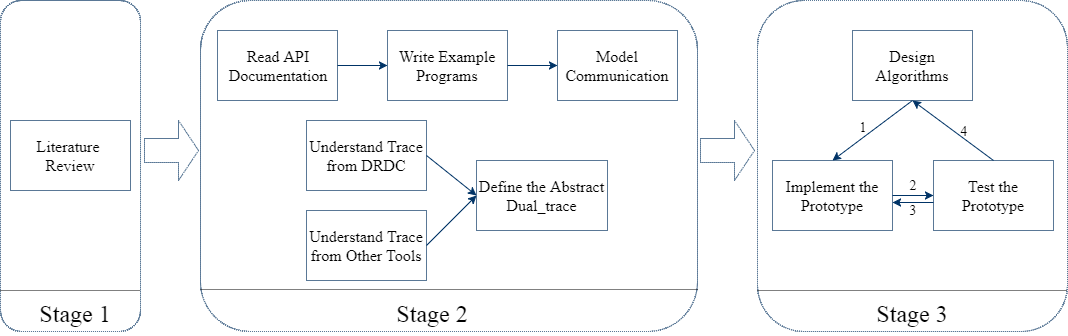
\includegraphics[scale=0.44]{Figures/methodology}}
  \caption{Research approach overview}
  \label{methodology}
  \end{figure}

This research requires background knowledge of software security and vulnerabilities. I acquired the background knowledge basically from literature review. It helped me acquire the essential concepts of software vulnerabilities and their categories, understand some facilities for vulnerabilities detection and software maintenance in the perspective of security. After that, I was convinced that communication analysis in assembly-level trace would benefit software security engineers to understand the behaviour of software and detect software vulnerabilities. 

In order to analyze the communication of programs, I had to know how the communication works. For this purpose, I started the investigation by writing simple example programs with the Windows API and run them locally in my desktop. By understanding their behaviour and reading the Windows API documentation, I abstracted the communication model which is not operating system specific.

The abstract assembly-level trace definition was built on the generalization of the trace format provided by our research partner, DRDC. I don't have the access to their home-made assembly-level tracer which is based on PIN\cite{_pin_????}. Fortunately, they provideed me with a comprehensive document about the format of the captured trace and example traces. With these, I grasped the constructive view of the assembly-level execution trace. Furthermore, some other tools can also capture the required information in assembly-level for communication analysis. This supports the generalization of the trace definition and the abstraction of the dual\_trace.

The implementation of the prototype and the communication analysis algorithms were developed in parallel. The high level communication identification algorithm and the specific algorithms for Named Pipe communication method were abstracted based on the implementation, while the others are developed theoretically. Two experiments are designed to test this analysis method, the prototype and some algorithms. 


\section{Contributions}
The main contributions of this work can be summarized as:
\begin{itemize}
  \item \textbf{Communication Model:} A communication model is abstracted from the understanding of several communication methods and is generic to other communication methods. This model indicates how the communication happen in terms of what information of it has been recorded. It can guide the software analyst to analyze the communication. The analyst might be able to retrieve some information of a communication from the traces, such as a sent function call in a trace with matched received function call from the other, or the transmitted messages. However, they might not aware that they can reconstruct the communication with all the essential information as a whole picture.

  \item \textbf{Dual\_trace and Functions Descriptor Formalization:} 

By understanding the assembly-level execution traces, a dual\_trace was formalized to describe the information that was needed for communication analysis. The dual\_trace formalization does not specify the format of the execution traces but defines what information is necessary to fulfil the analysis requirement. All execution traces that comply with this formalization can be used for the analysis. This formalization can be a reference for the design of assembly-level tracer, guiding \DIFdelbegin \DIFdel{them }\DIFdelend what information the tracer should capture to fulfil communication analysis.

The functions descriptor describes a communication method. Following the functions descriptor formalization, the user can develop a functions descriptor through understanding the mechanism of the communication method.

  \item \textbf{Communication Analysis Approach:} The overall approach to identify the communications in the dual\_trace is designed. Eight algorithms were developed for the components in this approach regarding some communication methods or communication types. 

  \item \textbf{Prototype:} A prototype for communication analysis through assembly-level execution traces is designed and implemented on Atlantis, which is an assembly-level execution traces analysis environment \cite{huang2017atlantis}. Atlantis has many features that benefit the communication analysis such as view synchronization and function inspection. Moreover, the unique memory state reconstruction feature makes the data verification of a communication much easier. After the user understand the communication model and the formalization presented in this thesis, the user can use the old Atlantis (without the implementation of this prototype) to perform the analysis. However, manually identifying the communication from two traces which might contain millions lines of instructions could be an extremely time consuming and exhausting task. This prototype makes the analysis much more efficient and practical. This prototype also demonstrates that the communication analysis approach is feasible. It is a unique tool for the security engineers to analyze the communications of programs via assembly-level execution trace analysis. 
\end{itemize}

\section{Thesis Organization}
In Chapter 2, I summarize the related background information and knowledge needed to understand or related to this work including security and vulnerability, program communication mechanisms, program execution trace tools, and Atlantis. 

Chapter 3 describes the model of the communication between two programs. This model defines the communication in the context of trace analysis and discusses the properties of the communications. 

In Chapter 4, I first present the abstract dual\_trace formulation. Based on this formulation, I describe the communication analysis process and the essential algorithms.

In Chapter 5, I present the implementation of a dual\_trace communication analysis prototype. 

In Chapter 6, I present two experiments of communication analysis with dual\_traces using the implemented prototype. Notably, the results show the communications are correctly identified. 

Finally, in Chapter 7, I conclude the result of this research and outline possible future works.
	\startchapter{Background}
\label{chapter:Bac}
In this chapter, I summarize the background related to this work. First I generally describe what is a software vulnerability. Second, I discuss the categorization of communications among programs. Third, I introduce some tools for assembly-level program debugging and analysis. Finally I introduce Atlantis, the existing assembly-level execution trace analysis environment, on which the prototype of this work is based.

\section{Software Vulnerability}
Software vulnerability detection is one of the use cases of communication analysis with assembly-level execution traces. Vulnerabilities, from the point of view of software security, are specific flaws or oversights in a program that can be exploited by attackers to do something malicious, such as modify sensitive information, disrupt or destroy a system, or take control of a computer system or program \cite{dowd_art_2006}. They are considered to be a subset of bugs. Input and data flow, interface and exceptional condition handling are where vulnerabilities most likely to surface in software. Memory corruption is one of the most common vulnerabilities. The awareness of these would make the security auditing and vulnerabilities detection have more clear focus. 

\section{Program Communications Categories}
Programs can communicate with each other via diverse mechanisms. The communication that happens among processes is known as inter-process communication. This refers to the mechanisms an operating system provides a process to share data with each other. It includes methods such as signal, socket, message queue, shared memory and so on \cite{garrido2000inter}. These communications can happen over a network or inside a device. Based on their reliability, the communication methods can be divided into two categories: reliable communication and unreliable communication. In this work, both communication methods are covered. However, I only discuss message based communication methods while leaving other communication methods such as remote procedural call for feature works.

\section{Program Execution Tracing at the Assembly-Level}
The communication analysis discussed throughout this thesis is based on assembly-level traces. Thus, capturing execution traces became a prerequisite of this work. DRDC has its own home-made tracer, and generated the traces used in the experiments of this research. However, the model and algorithms developed in this research are not limited to this specific home-made tracer. Any tracer that can capture sufficient information according to the model can serve this purpose.

There are many tools that can trace a running program at the assembly instruction level.  IDA Pro \cite{eagle_ida_2008} is a widely used tool in reverse engineering which can capture and analyze system level execution traces. Through open plugin APIs, IDA Pro allows plugin such as Codemap \cite{_c0demap/codemap:_????} to provide more sufficient features for ``run-trace" visualization. PIN \cite{_pin_????} is a tool for the instrumentation of programs, provides a rich API which allows users to implement their own tool for instruction trace and memory reference trace. Other tools like Dynamic \cite{brueningqz} and OllyDbg \cite{yuschuk2007ollydbg} also provide debugging and tracing functionality at the assembly-level. 

\section{Atlantis}
Atlantis is a trace analysis environment developed in the Chisel lab at the University of Victoria \cite{huang2017atlantis}. It can support analysis for multi-gigabyte assembly-level traces. There are several features that distinguish it from all other existing tools and make it particularly successful in large scale trace analysis. These features are 1) reconstruction and navigation the memory state of a program at any point in a trace; 2) reconstruction and navigation of system functions and processes; and 3) a powerful search facility to query and navigate traces \cite{huang2017atlantis}. The work of this thesis is not an extension of Atlantis. But it takes advantage of Atlantis by reusing its existing features to assist the dual\_trace analysis. The reason that I choose Atlantis for communication analysis is not because it was develop by the research group I work in, but the features that it already has make the implementation of the communication analysis prototype much easier than developing a new tool or use some other existing tool such as IDA Pro.





    \externaldocument{../appendix/chapter_app}
\startchapter{Communication Modeling}
\label{chapter:mod}
In this chapter, I model the communication of two running programs from the trace analysis point of view. The modeling is based on the investigation of some common used communication methods. But the detail of the communication methods will be discussed later in the algorithm and implementation chapters. This chapter only present the abstract communication model regarding the two communication categories: reliable and unreliable communications. 

\section{Communication Methods Categorization}
In terms of their reliability of data transmission, the communications can be divided into two categories: reliable and unreliable. \DIFdelbegin \DIFdel{A reliable communicationguarantees }\DIFdelend \DIFaddbegin \DIFadd{In a reliable communication, }\DIFaddend the data being sent by one endpoint through the channel is always received losslessly and in the same order in the other endpoint. \DIFdelbegin \DIFdel{However, in }\DIFdelend \DIFaddbegin \DIFadd{In }\DIFaddend some reliable communication, the sent packets can be re-segmented and arrives at the receiver end. In contrast, an unreliable communication does not guarantee the data being sent always arrives at the receiver end. Moreover, the data packets can arrive in any order. However, the positive side of the unreliable communications is that the packets always arrives as the original packets, no data re-segmentation happens. An endpoint is an instance in a program at which a stream of data is sent, received or both (e.g., a socket handle for TCP or a file handle for the named pipe). A channel is a conduit connecting two endpoints through which data can be sent and received. \DIFaddbegin \DIFadd{The categorization here doesn't consider if the physical medium used for the communication is lossless. It stands in the application point of view and see how much reliability of the communication methods the protocol can provide. For example, packets can be loss during the transmission in TCP channels. However, the protocol is designed to try its best to guarantee the losslessness by re-transmission, congestion control, etc. So from the point of view of the application, all data transmitted is controlled in an orderly fashion, is received in the correct order and is intact. }\DIFaddend Table \ref{methodsInCategories} gives examples of how communication methods fall in these two categories.
\begin{table}[H]
\centering
\caption{Communication method examples in two categories}
\label{methodsInCategories}
\begin{tabular}{|l|l|}
 \hline
\textbf{Reliable Communication}& \textbf{Unreliable Communication}\\
 \hline
Named Pipes & Message Queue   \\
TCP &  UDP \\
 \hline
\end{tabular}
\end{table}


\section{Communication Model}\label{definition}
The communication of two programs is defined in this section. The communication in this work is data transfer activities between two running programs through a specific channel. Some collaborative activities between the programs such as remote procedure call is out of the scope of this research. Communication among multiple programs (more than two) is not discussed in this work. The channel can be reopened to start new communications. However, the reopened channel is considered as a new communication. The model is not about how the communication works but what it looks like. There are many communication methods in the real world and they are compatible to this communication definition. 

\subsection{Communication Definition}
In the context of a dual\_trace, a communication is a sequence of data transmitted between two endpoints through a communication channel. I, therefore, defined a communication $c$ as a triplet:

$c =<ch, e_0, e_1>$

where $e_0$ and $e_1$ are endpoints while $ch$ is the communication channel (e.g., a named piped located at /tmp/pipe).

From the point of view of traces, the endpoints $e_0$ and $e_1$ are defined by three properties: the handle created within a process for the endpoint for subsequent operations (e.g. data send and receive), the data stream received and the data stream sent. Therefore, I define an endpoint $e$ as a triplet:

$ e =<handle, d_r, d_s>$

where $handle$ is the handle identifier, $d_r$ is the data stream received and $d_s$ is the data stream sent. A data stream is a sequence of sent packets or a sequence of received packets. Each packet $pk$ contains data that is being sent or received (its payload). Hence, we can define a data stream $d$ as a sequence of $n$ packets:

$ d = (pk_1, pk_2, ..., pk_n)$ 

Note: This is the sequence of packets as seen from the endpoint and might be different than the sequence of packets seen in the other endpoint, specially where there is packet reordering, loss or duplication.

Each packet $pk$ has two attributes:
\begin{itemize}
\item \textit{Relative time (it was sent or received):} In a trace, we do not have absolute time for an event. However, we know when an event (i.e., open, close, sending or receiving a packet) has happened with respect to another event. I use the notation 

$time(pk)$

to denote this relative time. Hence, 

if  $i < j $ , then  $time(pk_i) < time(pk_j)$

\item \textit{Payload:} Each packet has a payload (the data being sent or received). I use the notation 

$pl(pk)$ 

to denote this payload. 

\end{itemize}


\subsection{Communication Properties}\label{properties}
The properties of the communications can be described based on the definition of the communication.

\subsubsection{Properties of reliable communication}\label{reliablepro}
A reliable communication guarantees that the data sent and received between a packet happens without loss and in the same order.

For a given data stream, we define the data in this stream as the concatenation of the payload of all the packets in this stream, in the same order, and denote it as $data(d)$.

Given $ d=<pk_1, pk_2, ..., pk_n>$, $data(d)=pl(pk_1) \cdot pl(pk_2)\cdot \ldots \cdot pl(pk_n)$

\begin{itemize}
 \item \textit{Content Preservation:} 

 For a given data stream, we define the data in this stream as the concatenation of the payload of all the packets in the order of sending or receiving in this stream, and denote it as $data(d)$. Given $ d=<pk_1, pk_2, ..., pk_n>$, $data(d)=pl(pk_1) \cdot pl(pk_2)\cdot \ldots \cdot pl(pk_n)$.

 For a communication, the received data of an endpoint should always be a prefix of (potentially equal to) the sent data of the other. In other words, for a communication $c = <ch, <h_0, dr_0, ds_0>, <h_1, dr_1, ds_1>>$, $data(dr_0)$ is a prefix of $data(ds_1)$ and $data(dr_1)$ is a prefix of $data(ds_0)$.

\item \textit{Timing Preservation:} 

At any given point in time, the data received by an endpoint should be a prefix of the data that has been sent from the other:

for a sent data stream of size $m$, $ds= <pks_1, pks_2, ... pks_m>$ that is received in data stream of size $n$, $dr = <pkr_1, pkr_2, ... pkr_n>$, for any $k \in {1..n}$, there must exist $j \in {1..m}$ such that $pks_j$ was sent before $pkr_k$ was received:

$time(pks_j) < time(pkr_k)$

and

$ data(<pkr_1, pkr_2, ..., pkr_k>)$ is a prefix of $data(<pks_1, pks_2, ..., pks_j>)$.

In other words, at any given time, the recipient can only receive at most the data that has been sent.

\end{itemize}

\subsubsection{Properties of unreliable communication}\label{unreliablepro}
In an unreliable communication, the properties are not a concern in the concatenation of packets. Instead, each packet is treated as independent of each other.
\begin{itemize}
 \item \textit{ Content Preservation:} 

A packet that is received should have been sent:

for a sent data stream of size $m$, $ds= <pks_1, pks_2, ... pks_m>$ that is received in data stream of size $n$, $dr = <pkr_1, pkr_2, ... pkr_n>$,  for any $pkr_j \in dr$ there must exist $pks_i \in ds$, we will say that the $pkr_j$ is the matched packet of $pks_i$, and vice-versa,  hence $match(pkr_j) = pks_i$  and $match(pks_i) = pkr_j$.

 \item \textit{Timing Preservation:}  

At any given point in time, packets can only be received if they have been sent:

for a sent data stream of size $m$, $ds= <pks_1, pks_2, ... pks_m>$ that is received in data stream of size $n$, $dr = <pkr_1, pkr_2, ... pkr_n>$, for any $k \in {1..n}$, $time(match(pkr_j)) < time(pkr_j)$.

In other words, the match of the received packets must has been sent before it is received.
\end{itemize}


In the following two examples, $h_0$ and $h_1$ are the handles of the two endpoints $e_0$ and $e_1$ of the communications. $ds_0$, $dr_0$ and $ds_1$, $dr_1$ are the data streams of the endpoints $e_0$ and $e_1$. 

Figure \ref{reliableexample} is an example of an reliable communication. 

\begin{figure}[H]
\centerline{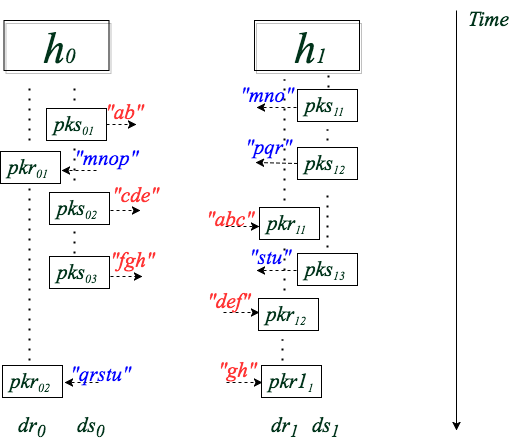
\includegraphics[scale=0.5]{Figures/reliableexample}}
\caption{Example of reliable communication}
\label{reliableexample}
\end{figure}

In this example, the payloads of the packets are:

$pl(pks_{01})=``ab"$, $ pl(pks_{02})=``cde"$, $pl(pks_{03})=``fgh"$;

$pl(pkr_{11})=``abc"$, $pl(pkr_{12})=``def"$, $pl(pkr_{13})=``gh"$ .

in one direction and 

$pl(pks_{11})=``mno"$, $pl(pks_{12})=``pqr"$, $pl(pks_{13})=``stu"$;

$pl(pkr_{01})=``mnop"$, $pl(pkr_{02})=``qrstu"$. 

on the other direction. 

By concatenating the payload of the sent packets in $ds_0$ and the received packets in $dr_1$, I notice that the concatenations are equal: 

$pl(pks_{01}) \cdot pl(pks_{02}) \cdot pl(pks_{03}) = pl(pkr_{11}) \cdot pl(pkr_{12}) \cdot pl(pkr_{13}) = ``abcdefgh"$ 

In the other direction, the concatenations of the payload of the sent packets in $ds_0$ and the concatenation of the received packets in $dr_1$ are equal:

$pl(pks_{11}) \cdot pl(pks_{12}) \cdot pl(pks_{13}) = pl(pkr_{01}) \cdot pl(pkr_{02}) = ``mnopqrstu"$. 

So this communication satisfy the content preservation. 

From the Figure \ref{reliableexample}, it is obvious that the relative time relationship of the packets are: 

$time(pks_{01}) < time(pks_{02}) < time(pkr_{11})< time(pks_{03}) < time(pkr_{12}) < time(pkr_{13}) $;

$time(pks_{11}) < time(pks_{12}) < time(pkr_{01})< time(pks_{13}) < time(pkr_{02})$. 

the fact that

$pl(pkr_{01}) = ``mnop"$ is the prefix of $pl(pks_{11}) \cdot  pl(pks_{12}) = ``mnopqr"$,

$pl(pkr_{01}) \cdot pl(pkr_{02})=``mnopqrstu"$ is the prefix of (in this case is identical to ) $pl(pks_{11}) \cdot pl(pks_{12}) \cdot pl(pks_{13}) = ``mnopqrstu" $,  

$pl(pkr_{11})=``abc"$ is the prefix of $pl(pks_{01} \cdot pl(pks_{02}) = "abcde"$,  

$pl(pkr_{11}) \cdot pl(pkr_{12})= ``abcdef"$ and  $pl(pkr_{11}) \cdot pl(pkr_{12}) \cdot pl(pkr_{13}) = ``abcdefgh"$ are  the prefix of  $pl(pks_{01}) \cdot pl(pks_{02}) \cdot pl(pks_{03})= ``abcdefgh"$

prove at any given time during this communication, the recipient only received at most the data that has been sent. So this communication satisfy the timing preservation. 


Figure\ref{unreliableexample} is an example of an unreliable communication. 

\begin{figure}[H]
\centerline{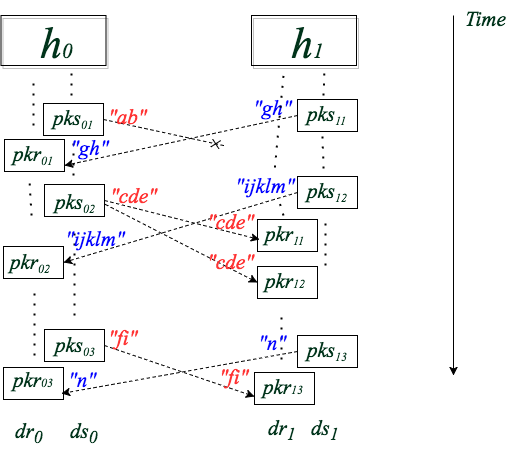
\includegraphics[scale=0.5]{Figures/unreliableexample}}
\caption{Example of unreliable communication}
\label{unreliableexample}
\end{figure}

In this example, the content preservation of the unreliable communication are satisfied since each received packet has a matched sent packet on the other side:

$pkr_{11} = pks_{02}=``cde"$; 

$pkr_{12} = pks_{02}=``cde"$;

$pkr_{13} = pks_{03}=``fi"$;

$pkr_{01} = pks_{11}=``gh"$;

$pkr_{02} = pks_{12}=``ijklm"$;

$pkr_{03} = pks_{13}=``n"$.

The timing preservation of the unreliable communication are satisfied since the match of the received packets (the sent packets) had been sent before the received packets are received.

$time(pkr_{11}) > time(pks_{02})$;

$time(pkr_{12}) > time(pks_{02})$; 

$time(pkr_{13}) > time(pks_{03})$;

$time(pkr_{01}) > time(pks_{11})$;

$time(pkr_{02}) > time(pks_{12})$;

$time(pkr_{03}) > time(pks_{13})$;





    \externaldocument{../3/chapter_modeling}
\externaldocument{../5/chapter_implementation}
\externaldocument{../appendix/chapter_app}
\startchapter{Communication Analysis}
\label{chapter:alo}
I defined a message transferring communication between two programs in Chapter \ref{chapter:mod}. The goal of this research is to develop a method to identify the communications from a dual\_trace. A dual\_trace is a pair of assembly-level execution traces of two interacting programs. In this chapter, I discuss the characteristics of the assembly-level execution trace, and then I formalize the dual\_trace. For all the traces that comply with this abstract dual\_trace formalization, the analysis approach presented in this chapter can be applied.


The process of the communication analysis is shown in Figure \ref{overview}. It takes the two traces in the dual\_trace as input and outputs the identified communications. In this overview figure, there are four components. The function call event reconstruction component will analyze the traces and try to reconstruct all function calls of the functions in the functions descriptor. These two sequences of events of these two traces will then flow into the stream extraction component separately. In each event sequence, the events might be triggered by different endpoints of different communications. I consider all the events triggered by the same endpoint as a stream. The stream extraction component will extract two sets of streams. After that, the stream matching component will take both of the stream sets as input and try to match them by their channel identifiers and output the potential identified communications. Finally, the data verification component will verify each communication and see if it satisfy the communication content preservation. Algorithms are designed separately for each component. Details about each elements and components of this overall process will be discussed in the following sections.


\begin{figure}[H]
\centerline{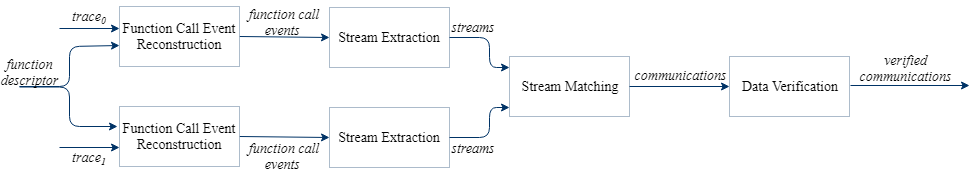
\includegraphics[scale=0.5]{Figures/overview}}
\caption{Process of the communication analysis through a dual\_trace}
\label{overview}
\end{figure}

\section{Dual\_Trace}\label{dualtrace}
In this section, I formalize a dual\_trace. All traces aligning with this formalization can be used as the input of the analysis process shown in Figure \ref{overview}. A dual\_trace consists of two assembly-level execution traces of two interacting programs. There is no timing information of these two traces which means we don't know the timing relationship of the events of one trace with respect to the other. However, the captured instructions in a trace are ordered in execution sequence. 

A dual\_trace is formalized as :

$dual\_trace = \lbrace trace_0, trace_1\rbrace$

where $trace_0$ and $trace_1$ are two assembly-level execution traces.

An execution trace consists of a sequence of instruction lines and can be defined as: 

$ trace = (l_1, l_2, ..., l_n)$ 

Each instruction line contains the executed instruction, the changed memory, the changed registers and the execution information and can be defined as a tuple:

$l = <ins, mch, rch, exetype, syscallInfo>$

where $ins$ is the instruction, $mch$ is the memory changes, $rch$ is the register changes, $exetype$ is the execution type which can be instruction, system call entry, and system call exit, $syscallInfo = <exeName, funcName>$ only appears when $exetype$ is system call entry or system call exit. $exeName$ is the executable file name (e.g., .dll and .exe), while $funcName$ is the name of a system function in this executable file.

Figure \ref{tracedefined} is an example of a piece of execution trace complying with the definition of a trace. 

\begin{figure}[H]
\centerline{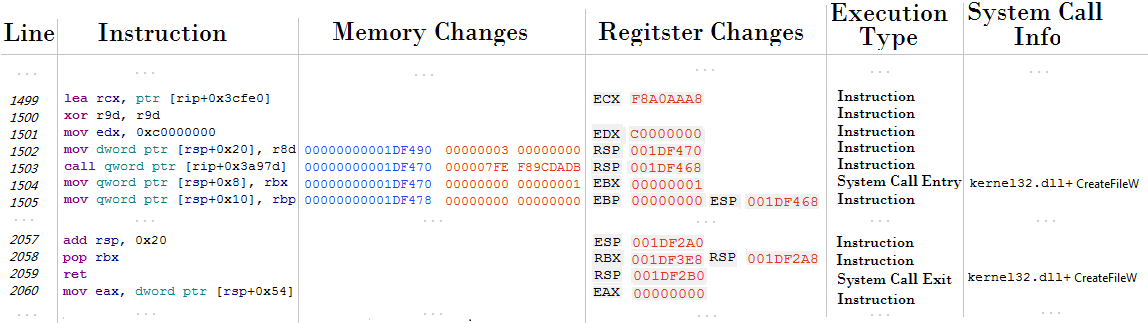
\includegraphics[scale=0.5]{Figures/tracedefined}}
\caption{An example trace }
\label{tracedefined}
\end{figure}



\section{Functions Descriptors}\label{cdesc}
There could be lots of function calls in an execution trace. However, most of them are not of interest. I am only concerned with the function call events of a specific communication method, such as TCP, UDP, and Named Pipe. To be able to identify and reconstruct the function calls, I define a functions descriptor as:

$cdesc = \lbrace fdesc_1, fdesc_2,...,fdesc_p \rbrace$

Each element, $fdesc$, is a function description and can be defined as:

$fdesc = < name, type, inparamdesc, outparamdesc >$

where, $name$ is the function name, $type$ is the function type which can be one of the four types: $open$, $close$, $send$ and $receive$. $inparamdesc$ is the input parameter descriptions illustrating how the registers and memory contents map to a list of parameters of interest (you might not care for all parameters of a function) of a given function call, and $outparamdesc$ is the output parameter descriptions similar to the input parameter descriptions. 

Table \ref{functionexample} is an example of a function description. In this example, the function name is $ReadFile$, it is a function for data receiving, so its function type is $receive$. The input parameter description has one concerned parameter, $Handle$, while the output parameter description has two parameters, ${RecvBuffer}$ and $MessageLength$. $Handle$ is a parameter which is a value stored in the register RCX. The $RecvBuffer$ is an address for the input message stored in the register RAX. The $MessageLength$ is a output value stored in register R9. The value of the input parameters can be retrieved from the memory state on the function call instruction line, while the value of the output parameters can be retrieved from the memory state on the function return instruction line. If a parameter is an address instead of a value, the address should be retrieved first, then the retrieved address should be used to find the buffer content in the memory state. The function description requires the understanding of the calling convention of the operating system. The Microsoft x64 calling convention can be found in Appendix \ref{convention}. More examples of communication method descriptions will be given in Chapter \ref{chapter:newsol}.

\begin{table}[H]
        \centering
        \caption{An example of a function description}
        \label{functionexample}
        \begin{tabular}{|l|l|l|l|l|l|l|l|}
            \hline
             \multirow{2}{*}{{\textbf{Name}}} & \multirow{2}{*}{{\textbf{Type}}} & \multicolumn{3}{c|}{\textbf{Input Parameter Description}} & \multicolumn{3}{c|}{\textbf{Output Parameter Description}} \\
              \cline{3-8} 
             & & \textbf{Name}& \textbf{Register} &  \textbf{Addr/Val} & \textbf{Name}& \textbf{Register} &  \textbf{Addr/Val}  \\
             \hline
             \multirow{2}{*}{ReadFile}
             &\multirow{2}{*}{receive} &  \multirow{2}{*}{Handle} & \multirow{2}{*}{RCX} & \multirow{2}{*}{Value} & RecvBuffer & RDX  & Addr\\
              \cline{6-8} 
             & & & & & MessageLength & R9  & Val\\
            \hline            
        \end{tabular}
    \end{table}

\section{Function Call Event Reconstruction Algorithm}
In last two sections, I formalized the assembly-level execution trace and defined the functions descriptor of a communication method. The functions descriptor helps to locate the function calls and retrieve the parameters of interest from an execution trace. These function calls contain the information of a communication, such as the channel identifier, the packets sent or received, etc. Before any communication can be identified, the function calls of that communication method have to be reconstructed first. 

In this section, I define the function call event and present an algorithm to reconstruct the function call events from an assembly-level execution trace. 

With the functions descriptor and the execution trace as input, the function call event reconstruction algorithm identifies the function call entry instruction line and reconstructs the input parameters from the memory state of that line. Then it identifies the function call exit line of the corresponding function call and reconstructs the output parameters from the memory state of the function exit line. After iterating through the whole execution trace, the algorithm outputs a sequence of function call events of length $m$. This sequence of events can be defined as $etr$:

$etr = (ev_1, ev_2, ..., ev_m)$

A function call event $ev$ in $etr$ is defined as a tuple:

$ev = <funN, inparams, outparams, type>$

where $funN$ is the function name, $inparas$ includes all the input parameters with the parameter name and value, $outparas$ includes all the output parameters, and $type$ is the event type which is inherited from the function description and can be one of the four types: $open$, $send$, $receive$ and $close$.


If the parameter is an address, the parameter's value is the string from the buffer pointed to by that address instead of the buffer address.

Algorithm \ref{eventAlg} presents the pseudocode for the function call event reconstruction algorithm. This algorithm is designed to reconstruct the function call events for one communication method. If multiple communication methods are being investigated, this algorithm can be run multiple times to analyze each of them. Since there are usually a small number of functions of interest for a communication method compared to the number of instruction lines in the execution trace, the time complexity of this algorithm is $O(N)$ and $N$ is the number of instruction lines in the trace.

\begin{algorithm}[H]
\DontPrintSemicolon
\caption{{\bf Function Event Reconstruction Algorithm} \label{eventAlg}}
\tcc{$trace$ is the assembly-level execution trace with a sequence of instruction lines: $(l_1, l_2, ..., l_n)$, $cdesc$ is the functions descriptor contains a set of function descriptions: $fdesc_1, fdesc_2, ..., fdesc_p$, $etr$ is a sequence of function call events}
\KwIn{ $trace, cdesc$}
\KwOut{$etr$}
$etr \leftarrow \emptyset$\; 
$i \leftarrow 1$\;
\tcc{Emulate the Execute of each instruction line of the trace}
\While{$i \leq n$}{
       $l \leftarrow trace[i]$\;
       $i \leftarrow i+1$\;
       Execute the instruction of $l$\;
     \For{$fdesc \in cdesc$}{
        \If{$l$ is a call to the function described by $fdes$}{
                Create an new function call event $ev$\;
                $ev.funN  \leftarrow fdesc.name$\;
                $ev.type  \leftarrow fdesc.type$\;
                Get the input parameters from the memory state and append them to  $ev.inparams$\;
                $i \leftarrow i+1$\;
                \While{$i \leq n$}{
                      $l \leftarrow trace[i]$\;
                      $i \leftarrow i+1$\;
                      Execute the instruction of $l$\;
                      \If{$l$ is a exit of the function described by $fdes$}{
                          Get the output parameters from the memory state and append them to  $ev.out params$\;
                          Break the inner while loop\;
                      }                     
                }
                $etr.append(ev)$\;
                Break the For loop\;
         }
}
}

\KwRet $etr$\;
\end{algorithm} 

An example of a sequence of function call events as the output of this algorithm is shown in Listing\ref{eventsexample}.

\DIFdelbegin %DIFDELCMD < \begin{lstlisting}%DIFDELCMD < [caption= Example of  $etr$, label=eventsexample]
%DIFDELCMD < {funN:CreateNamedPipe, type:open,inparams:{Handle:18, FileName:mypipe}, outparams:{}},
%DIFDELCMD < {funN:CreateNamedPipe, type:open,  inparams:{Handle:27,  FileName:Apipe}, outparams:{}},
%DIFDELCMD < {funN:WriteFile, type:send, inparams:{Handle:27, SendBuf:Message1}, outparams:{MessageLen:9}},
%DIFDELCMD < {funN:WriteFile, type:send, inparams:{Handle:27, SendBuf:Message2}, outparams:{MessageLen:9}},
%DIFDELCMD < {funN:ReadFile, type:receive, inparams:{Handle:27}, outparams:{RecvBuf:Message3, MessageLen:9}},
%DIFDELCMD < {funN:CloseHandle, type:close, inparams:{Handle:27}, outparams:{}},
%DIFDELCMD < \end{lstlisting}
%DIFDELCMD < %%%
\DIFdelend \DIFaddbegin \begin{lstlisting}[caption= Example of  $etr$, label=eventsexample]
{funN:CreateNamedPipe, type:open,inparams:{Handle:18, FileName:mypipe}, outparams:{}},
{funN:CreateNamedPipe, type:open,  inparams:{Handle:27,  FileName:Apipe}, outparams:{}},
{funN:WriteFile, type:send, inparams:{Handle:27, SendBuf:Message1}, outparams:{MessageLen:9}},
{funN:WriteFile, type:send, inparams:{Handle:27, SendBuf:Message2}, outparams:{MessageLen:9}},
{funN:ReadFile, type:receive, inparams:{Handle:27}, outparams:{RecvBuf:Message3, MessageLen:9}},
{funN:CloseHandle, type:close, inparams:{Handle:27}, outparams:{}}
\end{lstlisting}
\DIFaddend 

\section{Channel Open Mechanisms}\label{mecha}
The channel open mechanism affects the stream extraction and stream matching strategy. So I discuss them before presenting those algorithms. The channel open mechanism of a named pipe and message queue is relatively simple. In the Windows implementation, only one function call is related to the handle identification of the stream. However, for TCP and UDP the mechanism is complicated.

In all communication methods, all operations such as packet send and receive use a handle as an identifier to bind them to an endpoint. This handle is generated or returned by a channel open function call and will be assigned to an input parameter for all other related function calls to indicate the corresponding endpoint. However, in other communication methods, the handles might have other names, such as file handle for Named Pipe or socket (sometime called socket handle) for UDP and TCP. All of these are essentially equivalent.

A handle is an unique identifier among all open endpoints. An open endpoint is one that can still be used for data transfer. For example, if there are ten endpoints opened for communications, the handles for all these ten endpoints are different. However, if any of these endpoints is closed, its handle can be reused for other newly created endpoints. Since the handle is the unique identifier for an endpoint and its related events, we need to know it to identify an endpoint and its corresponding function call events. 

Moreover, since two endpoints (one from each trace) are connected to a channel for communication, each endpoint has to know the identifier of the channel to connect to it. This channel identifier is usually given to the endpoint in the channel open function calls. The endpoint will remember this channel and know where the data should be sent to and received from. Therefore, to identify a communication, the channel identifier given to an endpoint needs to be found during the channel open stage.

In the following subsections, I will explain how the different communication methods open their channels for communication.

\subsection{Named Pipe Channel Open Mechanisms} 
In the Named Pipe communication method, a named pipe server is responsible for the creation of the pipe. The creation of a named pipe returns the file handle of that pipe. So on the server side, the identification of the stream needs to identify the pipe creation function call. Clients can connect to the pipe with the pipe name after it is created. So, on the client side, the identification of the stream is to identify the pipe connection function call. The handle returned by the pipe creation and connection function calls will be used later when data is being sent to or received from a specified pipe. In a named pipe, the file is used as the media of the channel, so the identifier in this case is the file name. \cite{WinNamedpipe} Figure \ref{namedpipeopen} exemplifies the channel set up process for a Named Pipe communication in Windows. 

\begin{figure}[H]
\centerline{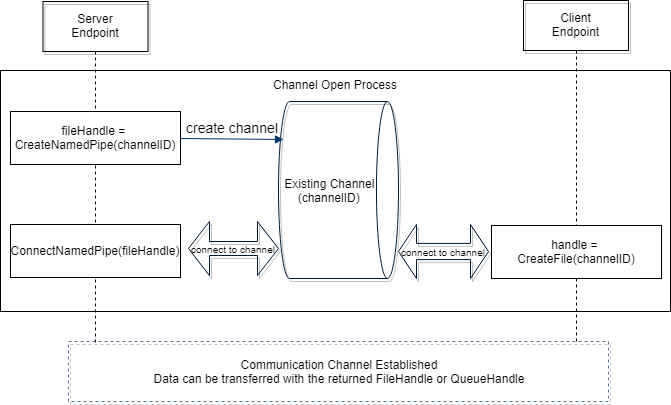
\includegraphics[scale=0.5]{Figures/namepipechannelopen}}
 \caption{Channel open process for a named pipe in Windows}
\label{namedpipeopen}
\end{figure}

\subsection{Message Queue Channel Open Mechanisms} 
For the Message Queue communication method, the endpoints of the communication can create the queue or use the existing one. However, both endpoints have to open the queue before accessing it. The handle returned by the open queue function will be used later when messages are being sent or received to indicate the corresponding endpoint. The identifier of the channel is the input for the open queue function. \cite{WinMSMQ} Figure \ref{msmqopen} exemplifies the channel set up process for a Message Queue communication in Windows.

\begin{figure}[H]
\centerline{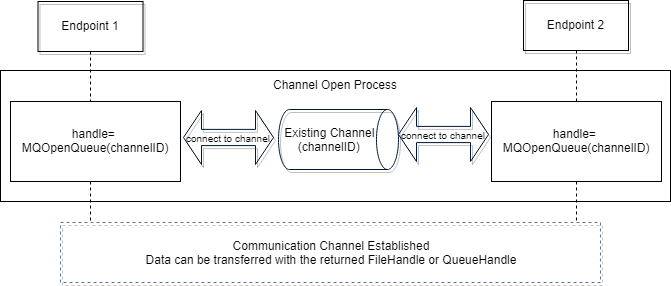
\includegraphics[scale=0.5]{Figures/msmqchannelopen}}
 \caption{Channel open process for a message queue in Windows}
\label{msmqopen}
\end{figure}

\subsection{UDP and TCP Channel Open Mechanisms} 
For the UDP and TCP communication methods, the communication channel is set up by both endpoints. The socket create function should be called on both endpoints. After the socket handles are created, the server endpoint binds the socket to its service address and port by calling the socket bind function. Then the server endpoint calls the listening function to accept the client connection. The client calls the connection function to connect to the server. When the listening function call returns successfully, a new socket handle will be generated and returned for further data transfer between the server endpoint and the connected client endpoint. After all these operations are performed successfully, the channel is established and the data transfer can start. During the channel open stage, server endpoint has two socket handles, the first one is used to listen to the connection from the client, and the second one is used for real data transfer. The server's address and port are considered to be the identifier of the channel \cite{winsock}. Figure \ref{channelopen2} exemplifies the channel open process for TCP and UDP in Windows.

\begin{figure}[H]
\centerline{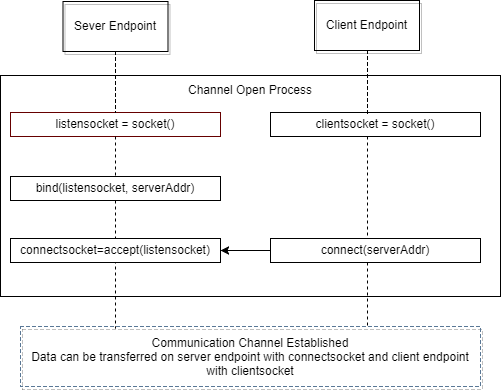
\includegraphics[scale=0.6]{Figures/tcpudpchannelopen}}
 \caption{Channel open model for TCP and UDP in Windows}
\label{channelopen2}    
\end{figure}

\section{Stream Extraction Algorithm}
The sequence of function call events output by the function call event reconstruction algorithm may belong to different endpoints. We need to further separate these events for each endpoint. Each subset of these events belonging to an endpoint is considered to be a stream. There are four types of events in each stream: open, send, receive and close. Hence, we can further divide a stream into substreams which are called open stream, send stream, receive stream, and close stream. There will be only one type of event in each of these streams. The reason to divide a stream into sub streams is that the later stream matching only \DIFdelbegin \DIFdel{need }\DIFdelend \DIFaddbegin \DIFadd{needs }\DIFaddend the information extracted from the open stream and the data verification only \DIFdelbegin \DIFdel{need }\DIFdelend \DIFaddbegin \DIFadd{needs }\DIFaddend the data extracted from the send and receive streams. So separating them will simplify the later processes. Since a stream corresponds to an endpoint and an endpoint is connected to a channel, it is necessary to know the endpoint handle and the channel identifier corresponding to this stream. 

A stream is formally defined as a tuple:

$s = <handle, channelId, so, ss, sr, sc>$

where $handle$ is the handle of the endpoint, $channelId$ is the identifier of the channel the endpoint of this stream is connected to, $so$ is the open stream, $ss$ is the send stream, $sr$ is the receive stream, $sc$ is the close stream. 

The sub streams $so$, $ss$, $sr$, $sc$ are sequences of events, $sx$ is defined as:

$sx = (ev_1, ev_2, ..., ev_p)$

The event numbering of in this sub stream is different from the original sequence of event. For example, $ev_1$ in $sx$ and $ev_1$ in $etr$ might be different events.

The stream extraction algorithms are designed to separate the streams from a sequence of function call events. In these algorithms, a stream is identified by the endpoint handle output by channel open function calls. Then all other events will be added to this stream.  According to the channel open mechanisms discussed in Section \ref{mecha}, the identifier of the channel and the handle of the endpoint can be retrieved from the channel open function call events.

The input of this algorithm is the sequence of events $etr = (ev_1, ev_2, ..., ev_n)$ from the function call event reconstruction algorithm. Since the events in $etr$ are reconstructed in sequence of the instructions which are ordered by the time of occurrence, the events are implicitly sorted by time of occurrence. 

The outputs of the stream extraction algorithms are a set of streams of size $p$, which can be defined as:

$str = (s_1, s_2, ..., s_p)$

According to the channel open mechanisms, two different algorithms are designed, one for Named Pipe and Message Queue, while the other for TCP and UDP. 

\DIFdelbegin \subsubsection{\DIFdel{Stream Extraction Algorithm for Named Pipe and Message Queue}}
%DIFAUXCMD
\addtocounter{subsubsection}{-1}%DIFAUXCMD
\DIFdelend \DIFaddbegin \subsection{\DIFadd{Stream Extraction Algorithm for Named Pipe and Message Queue}}
\DIFaddend This algorithm is designed for the extraction of the streams for Named Pipe and Message Queue. Since for each endpoint of the communication, only one channel open function call is needed to identify the endpoint, it is simple to identify the stream once the endpoint handle is found. 

The same handle may be reused by another endpoint once it is closed by the channel close function call. Therefore, before the detection of the channel close function call, if a new channel open function call with the same returned handle is detected, the second channel open is treated as an error. The error handling is not discussed in this algorithm. This algorithm recognizes this error by having $tempstreams$ to keep track of the streams that are still open. Once the stream is closed, this stream will be removed from $tempstreams$. The time complexity of this algorithm is $O(N)$ , $N$ is the number of events in the trace.

\begin{algorithm}[H]
\DontPrintSemicolon
\caption{{\bf Stream Extraction Algorithm for Named Pipe and Message Queue} \label{streamext1}}
\tcc{$etr$ is a sequence of function call events output by Algorithm \ref{eventAlg}; $str$ is a set of streams corresponding to a set of endpoints}
\KwIn{$etr$}
\KwOut{$str$} 
$str \leftarrow \emptyset$\; 
\tcc{a temporary stream set for all open streams}
$tempstreams \leftarrow \emptyset$\;
\For{$ev \in etr$}{
   \If{$ev.type = open$ }{
         $h \leftarrow$the handle in $ev.outparams$\;
         \If{$tempstreams[h]$ not exist}{
         $tempstreams[h] \leftarrow$ a new $s$\;
         $tempstreams[h].handle \leftarrow h$\;
         $tempstreams[h].channelId \leftarrow$ the channel identifier from $ev.inparams$\; 
         $tempstreams[h].so.append(ev)$\;   
         }
   }
   \ElseIf{$ev.type = send$}{    
   $h \leftarrow$the handle in $ev.inparams$\;  
          \If{$tempstreams[h]$ exist}{
         $tempstreams[h].ss.append(ev)$\;
         }
   }
   \ElseIf{$ev.type = receive$}{    
   $h \leftarrow$ the handle in $ev.inparams$\;  
          \If{$tempstreams[h]$ exist}{
         $tempstreams[h].sr.append(ev)$\;
         }
   }
      \ElseIf{$ev.type = close$}{    
   $h \leftarrow$ the handle in $ev.inparams$\;  
          \If{$tempstreams[h]$ exist}{
         $tempstreams[h].sc.append(ev)$\;
         $str.append(tempstreams[h])$\;        
         remove $tempstreams[h]$ from $tempstreams$\;
         }
   }
   \Else{
    unknown event type error\;
   }       
}
\KwRet $str$\;
\end{algorithm} 

\DIFdelbegin \subsubsection{\DIFdel{Stream Extraction Algorithm for TCP and UDP}}
%DIFAUXCMD
\addtocounter{subsubsection}{-1}%DIFAUXCMD
\DIFdelend \DIFaddbegin \subsection{\DIFadd{Stream Extraction Algorithm for TCP and UDP}}
\DIFaddend This algorithm is designed for extracting the streams for TCP and UDP. In the channel open stage, socket handles are created by function calls of the socket create function in both client and server. On the server side, this created socket is only used for listening to the client's connection. The listening is accomplished by calling the accept function. One of the input parameters of the accept function call is the listening socket handle, and the output of it is a new data transmission socket handle. 


In this algorithm, each created socket will be identified as a stream. The two socket handles in the server side are considered to be two handles for two streams, the stream identified by the listening handle is called the parent stream and the one identified by the data transmission handle is called the child stream. The events in the parent stream contain the information needed for stream matching algorithm for the child stream later, so the child stream will inherit all the events from its parent. 

Similar to the algorithm for Named Pipe and Message Queue, the reuse of a handle can only happen after a stream identified by this handle is closed. Otherwise the handle reuse will be treated as an error. The error handling is not discussed in this algorithm. A set, $tempstreams$, is also used in this algorithm to check for the open streams.

The time complexity of this algorithm is also $O(N)$, $N$ is the number of events in the trace.

\begin{algorithm}[H]
\caption{{\bf Stream Extraction Algorithm for TCP and UDP} \label{streamext2}}
\tcc{$etr$ is a sequence of function call events output by Algorithm \ref{eventAlg}; $str$ is a sequence of streams corresponding}
\KwIn{$etr$}
\KwOut{$str$} 
$str \leftarrow \emptyset$\; 
\tcc{a temporary stream set for all open streams}
$tempstreams \leftarrow \emptyset$\;
\For{$ev \in etr$}{
   \If{$ev.funN = socket$}{
      $h \leftarrow$ the handle in $ev.outparams$\;
      \If{$tempstreams[h]$ not exist}{
         $tempstreams[h] \leftarrow$ a new $s$\tcp*[f]{a new stream}\;
         $tempstreams[h].handle \leftarrow h$\;
         $tempstreams[h].so.append(ev)$\;
      }     
   }  
   \ElseIf{$ev.funN = bind$ or $ev.funN = connect$}{
      $h \leftarrow$ the handle in $ev.inparams$\;
      \If{$tempstreams[h]$ exist}{
         $tempstreams[h].channelId \leftarrow$ address and port parameter in $ev.inparams$\;
         $tempstreams[h].so.append(ev)$\;
      }     
   }   
   \ElseIf{$ev.funN = accept$}{
      $h \leftarrow$ the handle in $ev.inparams$;\tcp*[f]{the handle of parent stream}\; 
      $hc \leftarrow$ the handle in $ev.outparams$;\tcp*[f]{the handle of child stream}\; 
      \If{$tempstreams[h]$ exist}{  
        \If{$tempstreams[hc]$ not exist}{
            $tempstreams[hc] \leftarrow$ a new $s$;\tcp*[f]{a new stream for the child}\; 
        }
         $tempstreams[hc].handle \leftarrow hc$\;
         $tempstreams[hc].channelId \leftarrow tempstreams[h].channelId$\;
         $tempstreams[hc].so.append(tempstreams[h])$;\tcp*[f]{append parent's events}\;           
         $tempstreams[hc].so.append(ev)$;\tcp*[f]{append the current event}\;  
      }     
   }     
   \ElseIf{$ev.type = send$}{  
      $h \leftarrow$ the handle in $ev.inparams$\;    
      \If{$tempstreams[h]$ exist}{
         $tempstreams[h].ss.append(ev)$\;
      }
   }
   \ElseIf{$ev.type = receive$}{  
      $h \leftarrow$ the handle in $ev.inparams$\;    
      \If{$tempstreams[h]$ exist}{
         $tempstreams[h].sr.append(ev)$\;
      }
   }
   \ElseIf{$ev.type = close$}{
      $h \leftarrow$ the handle identifier from $ev.paras$\;
      \If{$tempstreams[h]$ exist}{
         $tempstreams[h].sc.append(ev)$\;
         $str.append(tempstreams[h])$\;        
         remove $tempstreams[h]$ from $tempstreams$\;
      }
   }      
   \Else{
      unknown event type or name error\;
   }   
}
\KwRet $str$\;
\end{algorithm} 


\section{Stream Matching Algorithm}\label{streammatch}
The function event extraction algorithm and the stream extraction algorithms work on a single execution trace. As defined before, a communication has two endpoints and each endpoint corresponds to a stream. To identify a communication from the dual\_trace, the two streams from that communication need to be found. 

The stream matching algorithm iterates over all the streams extracted from both traces of a dual\_trace and tries to match one stream of a trace to a stream of the other trace using the channel identifier held by each stream.

The channel identifiers held by the streams are retrieved in the stream extraction algorithm and are different for different communication methods. For TCP and UDP, the channel identifier is the server's address and port. For Named Pipe, the channel identifier is the file name, while for Message Queue, the channel identifier is the queue name.  

 The inputs of this algorithm are two sequence of streams $str_0$ and $str_1$ which are output by the stream extraction algorithm. The output of this algorithm is a sequence of the preliminary communications $cs$ of two matched streams. Each matched item in it is a triple $<channelId, s_0, s_1>$, where $channelId$ is the identifier of the channel, while $s_0$ and $s_1$ are the streams from $trace_0$ and $trace_1$ that correspond to the communication performed by each program on that channel. The time complexity of this algorithm is $O(N*M)$, $N$ and $M$ are the number of streams in both traces.

 \begin{algorithm}[H]
\DontPrintSemicolon
\caption{{\bf Stream Matching Algorithm for Named Pipe and Message Queue} \label{matchAlg}}
\tcc{$str_0$ and $str_1$ are two sequences of streams from $trace_0$ and $trace_1$. $cs$ is a sequence of preliminary communications}
\KwIn{$str_0, str_1$}
\KwOut{$cs$}
$cs \leftarrow \emptyset$\; 
\For{$s_0 \in str_0$}{
   \For{$s_1 \in str_1$}{     
     \If{$s_0.channelId = s_1.channelId$}{
            Create a new communication $c \leftarrow <channelId, s_0, s_1>$\;
            $cs.append(c)$\; 
      }
   }
}
\KwRet $cs$\;
\end{algorithm} 

This matching algorithm is not fully reliable. There are two situations in which the matching will fail. Take Named Pipe for example, the named pipe server is connected by two clients (client1 and client2) using the same file. The server trace and the client1 trace are analyzed as a dual\_trace, while the server trace and the client2 trace are analyzed as the other dual\_trace. In the server trace, there are two streams found. In each client trace, there is one stream found. For the dual\_trace of the server and client1, there will be two possible identified communications, one is the real communication for server and client1, while the other is an error which actually is for server and client2. The stream in client1's trace will be matched by the two streams in the server's trace. 

The second situation is when the same channel is reused by the different endpoints in the same program. For example, the Named Pipe server and client finished the first communication and then closed the channel. After a while they re-open the same file again for another communication. The matching is based on the identifiers, so in this case, there will be two matchings.

Similar situations can also happen with the Message Queue, TCP and UDP communication methods. 

The data verification algorithm discussed in next section can reduce these errors. 

\section{Data Verification Algorithm}\label{verfication}
In the last section, I presented the stream matching algorithm and described the situations in which the matching can go wrong. In this section, I present the algorithms that verifies if the data in the two streams of a preliminary identified communication satisfies the communication preservation properties of the communication model in Chapter \ref{chapter:mod}. 

The data transfer characteristics divide the communications into reliable and unreliable categories. Named Pipe and TCP fall in the reliable category while Message Queue and UDP fall in the unreliable one. The properties of the model consist of content preservation and timing preservation. The verification should cover both preservation properties: 
\begin{itemize}
\item verify the content preservation of the data in the matched streams. 
\item verify the timing preservation of the data in the matched streams. 
\end{itemize}

To verify the timing preservation, the relative time of the events in both streams is needed. Unfortunately, we can only determine the relative time in a stream but not crossing two streams. So it's unfeasible to verify the timing preservation property for neither reliable nor unreliable communications. The verification algorithms discussed in this section will only cover the content preservation property.  

The inputs of the data verification algorithms are two preliminary matched streams $s_0$ and $s_1$. The output is a boolean indicating if the streams satisfy content preservation. All communications that don't satisfy the content preservation should be excluded as identified communications.

For each communication method the verification of the corresponding preservation is applied, That is, for Named Pipe and TCP, the reliable communication preservation needs to be verified and for Message Queue and UDP, the unreliable communication preservation needs to be verified. The following sub sections present the versification  algorithms for these four communication methods. In each sub section, I discuss the data transfer properties and scenarios of the communication method and then present the verification algorithm. \DIFaddbegin \DIFadd{The data transfer properties and scenarios are summarized from the perspectives of the how the protocol normally behave. So the output communications after data verification are those aligning with the those normal communication properties. By comparing the output extracted streams and the communications, the software security engineer might be able to detect the malicious streams and further detect the problems from the programs.
}\DIFaddend 

\subsection{Data Verification Algorithm for Named Pipe}
Named Pipe provides First In First Out (FIFO) communication mechanism for inter-process communication. It can be a one-way or a duplex pipe \cite{WinNamedpipe}. The basic data transfer characteristics of Named Pipe are: 
\begin{itemize}
  \item Bytes are received in order;
  \item Bytes sent as a segment can be received in multiple segments (the opposite is not true);
  \item No data duplication;
  \item If a sent segment is lost, all the following segments will be lost (this happens when the receiver disconnects from the channel).

\end{itemize}

Based on these characteristics, the data transfer scenarios of Named pipe can be exemplified in Figure \ref{namedpipe}. 
\begin{figure}[H]
\centerline{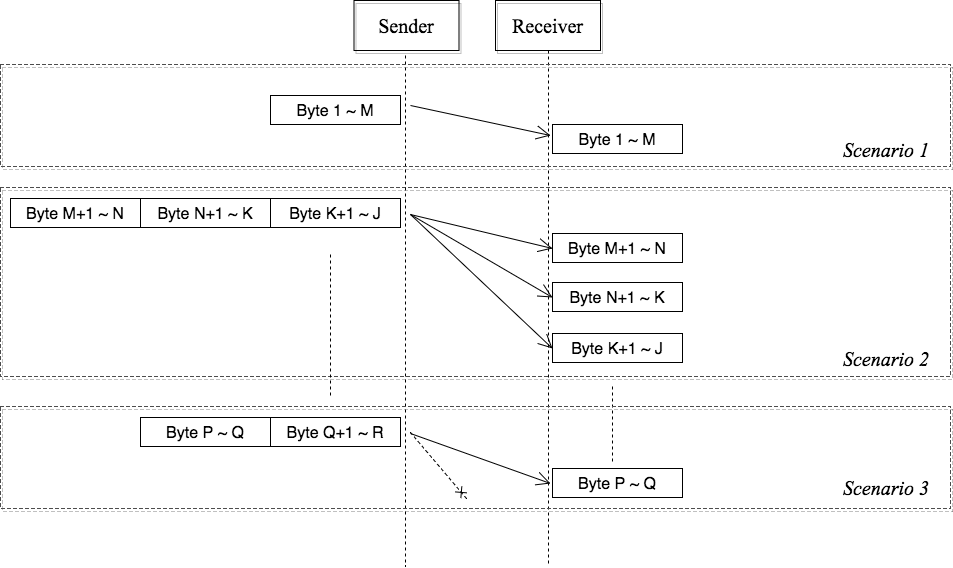
\includegraphics[scale=0.4]{Figures/namedpipe}}
\caption{Data transfer scenarios for Named Pipe}
\label{namedpipe}
\end{figure}

The content preservation verification is trivial. It compares the concatenation of the packet content of the sent events in a stream to the concatenation of the packet content of the receive events in the other stream, which is presented in Algorithm \ref{dataAlg1}. Since the concatenation needs to inspect the events in the streams, the time complexity of this algorithm is $O(N)$, $N$ is the total number of data transfer events in the two streams.

\begin{algorithm}[H]
\DontPrintSemicolon
\caption{{\bf Data Verification of Named Pipe} \label{dataAlg1}}
\tcc{$s_0$ and $s_1$ are two matched streams from $trace_0$ and $trace_1$. The output boolean $satisfied$ is true if the matched stream satisfy the content preservation of a communication.}
\KwIn{$s_0, s_1$}
\KwRet{$satisfied$}\;
$send_0 \leftarrow$ concatenation of the payload of send function call events in $s_0.ss$;\;
$send_1 \leftarrow$ concatenation of the payload of send function call events in $s_1.ss$;\;
$receive_0 \leftarrow$ concatenation of the payload of receive function call events in $s_0.sr$;\;
$receive_1 \leftarrow$ concatenation of the payload of receive function call events in $s_1.sr$;\;
\KwRet{$receive_1$ is prefix of $send_0$ AND $receive_0$ is prefix of $send_1$ }
\end{algorithm} 

\subsection{Data Verification Algorithm for TCP}
TCP is the most basic reliable transport method in computer networking. TCP provides reliable, ordered, and error-checked delivery of a stream of octets between applications running on hosts in an IP network. The TCP header contains the sequence number of the sending octets and the acknowledgement sequence this endpoint is expecting from the other endpoint(if ACK is set). The basic data transfer characteristics of TCP are:
\begin{itemize}
  \item Bytes received in order;
  \item No data lost (lost data will be re-transmitted);
  \item No data duplication;
  \item Bytes sent in packet and received in packet, no re-segmentation.
\end{itemize}

Based on these characteristics,  the data transfer scenarios of TCP can be exemplified in Figure \ref{tcp}.

\begin{figure}[H]
\centerline{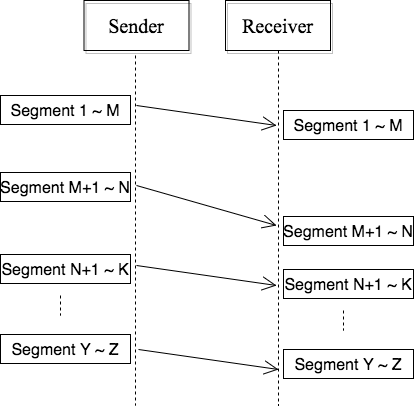
\includegraphics[scale=0.4]{Figures/tcp}}
 \caption{Data transfer scenarios for TCP}
\label{tcp}
\end{figure}

According to the data transfer properties of TCP, all packets sent in one side will be received in the same other in the other side. The verification can be restricted to packet to packet. If every $i-th$ send event in a stream can be matched by the $i-th$ receive event in the other stream for both directions, we can assert that the content preservation is satisfied for the communication. The verification algorithm of TCP is presented in Algorithm \ref{dataAlg2}. The time complexity of this algorithm is also $O(N)$, $N$ is the number of data transfer events in a stream.

\begin{algorithm}[H]
\DontPrintSemicolon
\caption{{\bf Data Verification of TCP} \label{dataAlg2}}
\tcc{$s_0$ and $s_1$ are two matched streams from $trace_0$ and $trace_1$. The output boolean $satisfied$ is true if the matched stream satisfy the content preservation of a communication.}
\KwIn{$s_0, s_1$}
\KwRet{$satisfied$}\;
\tcc{There is a chance that the trace capturing end before the channel is closed}
\For{$i \in {0..min(s_0.ss.size, s_1.sr.size)}$}{
     \If{$s_0.ss[i].payload\; \; != s_1.sr[i].payload$}{
       \KwRet False;\;
   }
}
\For{$i \in {0..min(s_1.ss.size, s_0.sr.size)}$}{
     \If{$s_1.ss[i].payload\; \;!= s_0.sr[i].payload$}{
       \KwRet False;\;
   }
}
 \KwRet True;\;
\end{algorithm} 


\subsection{Data Verification Algorithm for Message Queue}
Message Queue is a communication method to allow applications which are running at different times across heterogeneous networks and systems that may be temporarily offline to communicate with each other. Applications communicate to each other through the queue. Multiple sending applications can send messages to one queue and multiple receiving applications can read messages from one queue \cite{redkar2004pro}. In this work, only the case of one sending application versus one receiving application is considered. A queue can be one-way or duplex. The basic data transfer characteristics of Message Queue are:
\begin{itemize}
  \item Bytes sent in one packet are received in one packet, with no bytes re-segmented;
  \item Packets can be lost;
  \item Packets received in order;
  \item No data duplication.
\end{itemize}
Based on these characteristics, the data transfer scenarios of Message Queue can be exemplified in Figure \ref{msmq}.
\begin{figure}[H]
\centerline{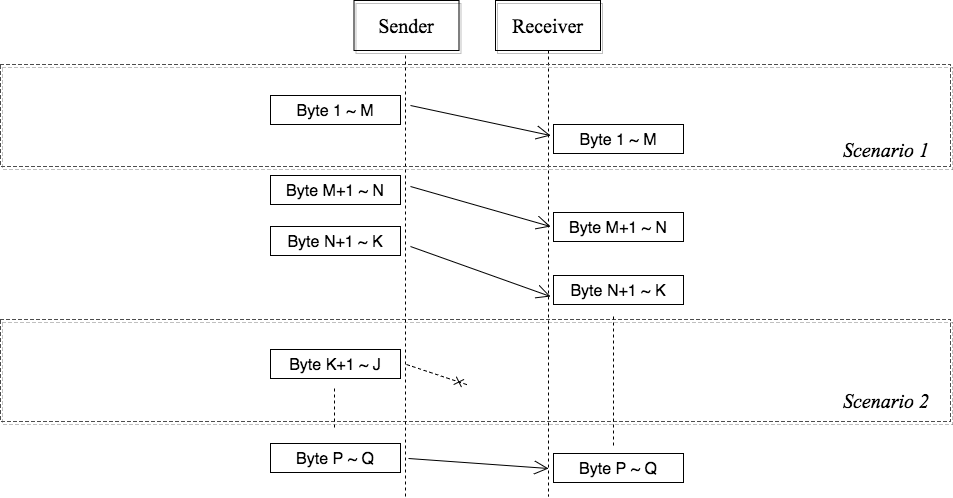
\includegraphics[scale=0.4]{Figures/msmq}}
\caption{Data transfer scenarios for Message Queue}
\label{msmq}
\end{figure}

To verify the content preservation of the unreliable communication, for each received packet, Algorithm \ref{dataAlg3} tries to find the matched sent packet in the other stream. If any of the received packets cannot be matched, the content preservation is not satisfied. Since the sent packets are received in order, the search for each received packet will start from the next index of the last matched sent packet. 

The time complexity of this algorithm is $O(N^2+M^2)$, $N$ and $M$ are the numbers of data sent events of the two streams.
\DIFdelbegin %DIFDELCMD < 

%DIFDELCMD < %%%
\DIFdelend 
\begin{algorithm}[H]
\DontPrintSemicolon
\caption{{\bf Data Verification of Message Queue } \label{dataAlg3}}
\tcc{$s_0$ and $s_1$ are two matched streams from $trace_0$ and $trace_1$. The output boolean $satisfied$ is true if the matched stream satisfy the content preservation of a communication.}
\KwIn{$s_0, s_1$}
\KwRet{$satisfied$}\;
\If{$s_0.ss.size < s_1.sr.size$ Or $s_1.ss.size < s_0.sr.size$ }{
   \KwRet False;\;
}
$lastMatchIndex = 0$;\;
\For{$i \in {0..s_1.sr.size}$}{
     $tempIndex = lastMatchIndex$;\;
     \For{$j \in {lastMatchIndex+1..s_0.ss.size}$}{
             \If{$s_0.ss[j].payload = s_1[i].sr.payload$}{
                      $lastMatchIndex \leftarrow j$;\;
                      break the inner For loop;\;
            }  
     }   
\tcc{This received packet cannot be matched by any sent packet}    
     \If{$tempIndex = lastMatchIndex$}{
                      \KwRet False;\;
            }     
}     
$lastMatchIndex = 0$;\;
\For{$i \in {0..s_0.sr.size}$}{
     $tempIndex = lastMatchIndex$;\;
     \For{$j \in {lastMatchIndex+1..sends_1.size}$}{
             \If{$s_1.ss[j].payload = s_0[i].sr.payload$}{
                      $lastMatchIndex \leftarrow j$;\;
                      break the inner For loop;\;
            }  
     }   
     \If{$tempIndex = lastMatchIndex$}{
                      \KwRet False;\;
            }     
}  
 \KwRet True;\;
\end{algorithm} 

\subsection{Data Verification Algorithm for UDP}
UDP is a widely used unreliable transmission method in computer networking. It is a simple protocol mechanism, which has no guarantee of delivery, ordering, or duplicate protection. This transmission method is suitable for many real time systems. The basic data transfer characteristics of UDP are:
\begin{itemize}
  \item Bytes sent in packet and received in packet, no re-segmentation;
  \item Packets can be lost;
  \item Packets can be duplicated;
  \item Packets can arrive receiver out of order.
\end{itemize}

Based on these characteristics, the data transfer scenarios of UDP can be exemplified in Figure \ref{upd}.
\begin{figure}[H]
\centerline{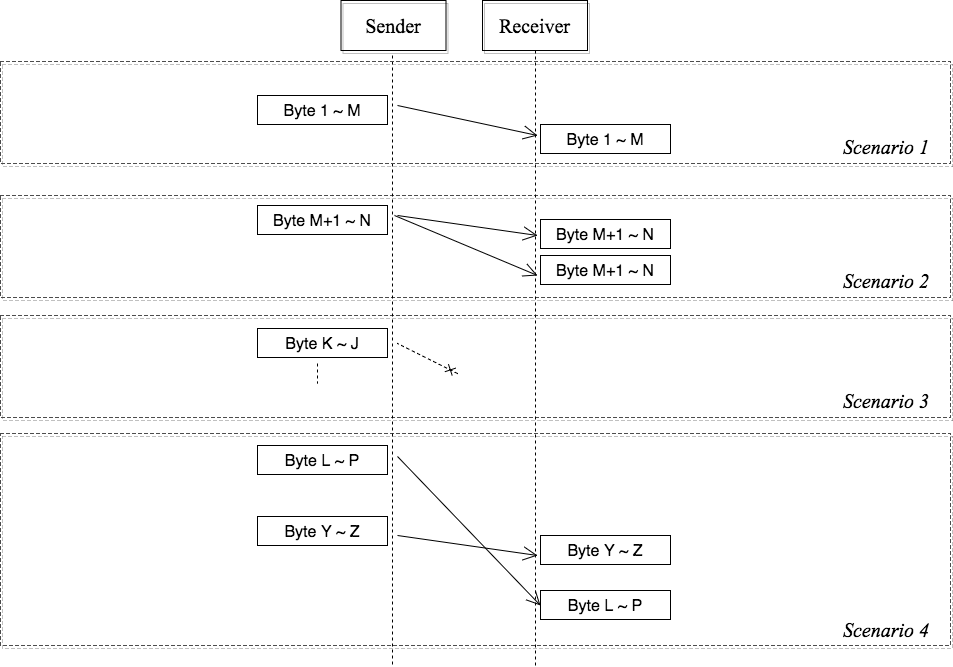
\includegraphics[scale=0.4]{Figures/udp}}
 \caption{Data transfer scenarios for UDP}
\label{upd}
\end{figure}

Similar to Message Queue, Algorithm \ref{dataAlg4} tries to match each received packet in one stream to the corresponding sent packet in the other stream. If any of the received packets cannot be matched, the content preservation is not satisfied. However, due to the potential reordering of packet, the matching is not restricted to the packet index (e.g, the $i-th$ received packet in one stream can be matched to the $j-th$ packet in the other stream, $i \neq j$). But the matched sent packet will be excluded from the following matching, which means each sent packet can only match to one received packet.

The time complexity of this algorithm is $O(N^2+M^2)$, $N$ and $M$ are the numbers of data sent transfer events in the two streams.
\DIFdelbegin %DIFDELCMD < 

%DIFDELCMD < %%%
\DIFdelend\begin{algorithm}[H]
\DontPrintSemicolon
\caption{{\bf Transmitted Verification of UDP} \label{dataAlg4}}
\tcc{$s_0$ and $s_1$ are two matched streams from $trace_0$ and $trace_1$. The output boolean $satisfied$ is true if the matched stream satisfy the content preservation of a communication.}
\KwIn{$s_0, s_1$}
\KwRet{$satisfied$}\;
\If{$s_0.ss.size < s_1.sr.size$ Or $s_1.ss.size < s_0.sr.size$ }{
   \KwRet False;\;
}
\tcc{For each received packet in stream $s_1$ try to find the sent packet in stream $s_0$. $s_1.sr$ is the sequence of received packet of stream $s_1$ while $s_0.ss$ is the sequence of sent packet of stream $s_0$}
\For{$i \in {0..s_1.sr.size}$}{
    $matchFlag = False$;\;
     \For{$j \in {0..s_0.ss.size}$}{
             \If{$s_0[j].ss.payload = s_1[i].sr.payload$}{
                      $matchFlag = True$;\;
                      delete the packet from $sends_0$
                      break the inner For loop;\;
            }  
     }   
\tcc{This received packet cannot be matched by any sent packet}
     \If{$matchFlag = False$}{
                      \KwRet False;\;
            }     
}  
\tcc{For each received packet in stream $s_0$ try to find the sent packet in stream $s_1$. $s_0.sr$ is the sequence of received packet of stream $s_0$ while $s_1.ss$ is the sequence of sent packet of stream $s_1$}   
\For{$i \in {0..s_0.sr.size}$}{
    $matchFlag = False$;\;
     \For{$j \in {0..s_1.ss.size}$}{
             \If{$s_1[j].ss.payload = s_0[i].sr.payload$}{
                      $matchFlag = True$;\;
                      delete the packet from $s_0.ss$
                      break the inner For loop;\;
            }  
     }   
     \If{$matchFlag = False$}{
                      \KwRet False;\;
            }     
} 
 \KwRet True;\;
\end{algorithm} 

\subsection{Limitation of the Data Verification}
The verification discussed in this chapter has two major limitations:
\begin{itemize}
    \item The timing preservation of the communication is not verified.
    \item Some mismatching cannot be excluded even with the content verification
\end{itemize}  

The reason that the timing preservation cannot be verified is lacking timing information across the two traces. 

For the second limitation, the main reason is that the data transmitted in two communications could be identical or very similar. 

In Section \ref{streammatch}, I described how one stream in one side of the dual\_trace can be matched by two or more streams on the other side. In order to reduce this type of error, I developed the data verification strategy and algorithms. However, in some cases, the transferred data of two communications can be identical or very similar. Even with content verification, the mismatched streams still cannot be excluded.

Figure \ref{secondlevelmatching} exemplifies this situation in a reliable communication analysis. Assuming that $s_{11}$, $s_{21}$ and $s_{22}$ have the same channel identifier, they will be matched as two communications (one consists of $s_{11}$ and $s_{21}$ while the other one consists of $s_{11}$ and $s_{22}$). Furthermore, $s_{21}$ and $s_{22}$ send and receive the exact data. So both of the communications are considered to satisfy the content preservation property. In this case, the algorithms will not be able to determine if  $s_{11}$ communicated with $s_{21}$ or $s_{22}$. There is no way from the analysis point of view to distinguish the actual communication. It's more reasonable to preserve all of them in the output and present them for the users to make the decision. The users might be able to distinguish them and find the valid one.


\begin{figure}[H]
\centerline{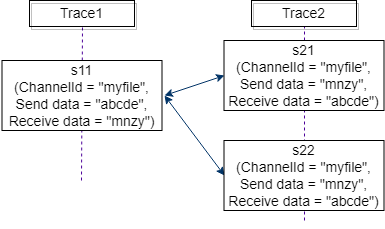
\includegraphics{Figures/secondlevelmatching}}
 \caption{An ineffective stream matching scenario}
\label{secondlevelmatching}
\end{figure}

\DIFaddbegin \section{\DIFadd{Discussion of Security Analysis Challenge}}
\DIFadd{Malware is a serious problem for all system nowadays. The intrusion of malware is generally an individual behavior, malwares attack the vulnerability of one or several specific systems, then intrudes into the system, destroys and controls it to obtains private information. Some malware can even be spread like a virus through the Internet, invading other systems with the same vulnerability. In general, malware is targeted at system-level intrusions, and there is very little damage to common application software unless there are obvious vulnerabilities that can be exploited for systematic attacks. \mbox{%DIFAUXCMD
\cite{leavitt2011mobile}
}\hspace{0pt}%DIFAUXCMD
}

\DIFadd{On the other hand, network attacks often occur on the network layer. Since the internet has be an extremely huge network in the world, the attack could be initiated at any network node. If there are no proper security measure, your data might be attacked during the transmission. There are many types of network attack, some are passive like monitoring information, some are active like corrupting and destroying the data or network itself. \mbox{%DIFAUXCMD
\cite{hansman2005taxonomy}
}\hspace{0pt}%DIFAUXCMD
}

\DIFadd{There is not a system that is absolutely secure from attackers. The running system's behaviour can change dramatically due to all of these attacks. The goal of the communication analysis is simply monitoring
programs in terms of data transmission. Perhaps the communication is modified by the attacks mention above. This places a huge challenge for communication analysis. For example, the identification of  a modified communication would be an extremely difficult mission. 
}

\DIFadd{However, even though there might be some cases that the communication can not be effectively identified, this work will still be valuable to the analyst, as it will show that the data sent was not received (at least the same data was not received) by the other side and might mean that the running environment is compromised.
}


	\DIFaddend \externaldocument{../3/chapter_modeling}
\externaldocument{../4/chapter_algorithm}
\startchapter{Dual\_trace Communication Analysis Prototype In Atlantis}
\label{chapter:newsol}
In this chapter, I present the design of the prototype of communication analysis from the dual\_trace. This prototype is implemented in Atlantis. Atlantis is an assembly-level execution trace analysis environment. It provides many features that benefit the communication analysis of dual\_trace. 

This prototype consists of four components: 1) declaring the functions descriptors of the communication methods, 2) a view that can display both traces in the dual\_trace in parallel, 3) implementation of the communication analysis algorithms for stream extraction and communication identification, and 4) a view for presenting the extracted streams and the identified communications from the dual\_trace.

\section{Use Cases}
In this section, two use cases are presented to depict how to use the developed components and the existing features of Atlantis to perform the communication analysis.

To analyze a dual\_trace, the user needs to perform the below operations in sequence:
\begin{itemize}
\item Open two traces in a parallel view (as part of this prototype)
\item Import the dynamic-linked library files for each trace (as part of the existing functionality of Atlantis)
\item Perform the stream extraction or communication identification operations (as part of this prototype)
\item Inspect the operation results by navigating the analysis results from the communication view (as part of this prototype).
\end{itemize}

Two use cases of this prototype are designed. The use case shown in Table \ref{usecase1} is for stream extraction. The goal of this use case is to analyze two execution traces in a dual\_trace and output the streams of each trace. The use case shown in Table \ref{usecase2} is for identifying the concerned communication from a dual\_trace. 

\begin{table}[H]
  \centering
  \caption{Use case 1: extract streams from a dual\_trace}
  \label{usecase1}
  \begin{tabular}{|l|p{13cm}|}
      \hline
       \textbf{Name} & Analysis streams of a communication method from the Dual\_trace\\
       \hline
       \textbf{Description} & A user capture two assembly-level execution traces of two interacting programs and needs to analysis them by extracting all communication streams of each of the traces and inspecting the extraction results \\
       \hline
              \textbf{Actor} & A software security engineer \\
       \hline
       \textbf{Precondition} & The user has two assembly-level execution traces and the .dll files of the systems where the programs of the captured traces were running\\
       \hline
       \textbf{Main Course}& 1. The user declares the functions descriptors for the communication methods of interest in a Json format setting file\\
        & 2. The user opens one of the trace in Atlantis\\
       &  3. The user opens the other trace as the dual\_trace of the first one\\
       & 4. The two opened traces are presented in the parallel view\\
       & 5. The user loads the related .dll files for both opened traces\\
       & 6. The user selects the operation ``Stream Extraction" in the ``Dual\_Trace Tool" menu.\\
       & 7. Atlantis prompts a dialog window giving the user all the communication methods in the functions descriptor setting file as options\\
       & 8. The user selects the communication methods that they want to analyze and click the ``OK" bottom\\
       & 9. Atlantis extracts the streams for both traces and lists the results in the ``Communication view"\\
       & 10. The user expands the result in the ``Communication view"\\
       & 11. The user selects one function call event in a stream and double clicks the entry\\
       & 12. Atlantis shows the corresponding instruction line in the trace and synchronizes all other views\\
      \hline               
  \end{tabular}
\end{table}


\begin{table}[H]
  \centering
  \caption{Use case 2: identify communications from the dual\_trace}
  \label{usecase2}
  \begin{tabular}{|l|p{13cm}|}
      \hline
       \textbf{Name} & Identify communications of a communication method from the Dual\_trace\\
       \hline
       \textbf{Description} & A user captures two assembly-level execution traces of two interacting programs and needs to analysis them by identifying all communications of the dual\_trace and inspects the extraction results \\
       \hline
              \textbf{Actor} & A software security engineer \\
       \hline
      \textbf{Precondition} & The user has two assembly-level execution traces and the .dll files of the systems where the programs of the captured traces were running\\
       \hline
       \textbf{Main Course}& 1. The user declares the functions descriptors for the communication methods of interest in a Json format setting file\\
        & 2. The user opens one of the trace in Atlantis\\
       &  3. The user opens the other trace as the dual\_trace of the first one\\
       & 4. The two opened traces are presented in the parallel view\\
       & 5. The user loads the related .dll files for both opened traces\\
       & 6. The user selects the operation ``Communication Identification" in the ``Dual\_Trace Tool" menu\\
      & 7. Atlantis prompts a dialog window giving the user all the communication methods in the functions descriptor setting file as options\\
       & 8. The user selects the communication methods that they want to analyze and click the ``OK" bottom\\
       & 9. Atlantis identifies the communications of the dual\_trace and lists the results in ``Communication view"\\
       & 10. The user expands the result in the ``Communication view"\\
       & 11. The user selects one function call event in a stream and double clicks the entry\\
       & 12. Atlantis shows the corresponding instruction line in the trace and synchronize all other views\\
      \hline               
  \end{tabular}
\end{table}

\section{Declaring of the Functions Descriptors}\label{functionset}
In Section \ref{cdesc}, I described how to develop a functions descriptor for each communication method. Each function description consists of four elements: 

$fdesc = \lbrace name, type, inparamdesc, outparamdesc \rbrace$

$name$ is the function name, $type$ can be $open$, $close$, $send$ and $receive$, $inparamdesc$ and $outparamdesc$ are the descriptions for the input and output parameters of interest. The communication analysis approach depicted in Chapter \ref{chapter:alo} can identify the communications described by the functions descriptor from the dual\_trace.

However, the functions descriptor for a communication method can be different depending on the implementation of the communication method in a program. Rather than hard coding the functions descriptors for the communication methods, this prototype loads the functions descriptors from a configuration file. A default template is given for reference. This template is generated by Atlantis when it is launched and stored in the .tmp folder of the trace analysis project. The users can modify this template to match the communication methods of interest. The default template example can be found in Appendix \ref{funcset}.

The functions descriptors in this configuration file will be the input for the stream extraction and communication identification features. When the user uses these two features, the list of the communication methods provided in the functions descriptor configuration file will be presented to them. They can select one or more communication methods to be analyzed. 

In the following subsections, functions descriptor examples are presented for reference. Other functions descriptors can be created by following the same method as developing the functions descriptor examples.

\subsection{Communication Methods' Implementation in Windows}\label{windows}
Learning the implementation of a communication is necessary to obtain the functions descriptor of the communication method. In this section, I present the results of analyzing the implementation of these four communication methods: Named Pipe, Message Queue, TCP and UDP in Windows. In the analysis, I reviewed the Windows APIs of the communication methods and their example code. By doing so, I obtained the functions descriptors of these methods. 

The Windows API set is very complex. Moreover, multiple solutions are provided to fulfil a communication method. It is not feasible within the scope of this thesis to enumerate all solutions for each communication method. I only investigated the most basic usage provided in the Windows documentation. For each communication method, a functions descriptor with a list of system function descriptions is provided for reference. The functions in the descriptors are supported in most Windows operating systems, such as Windows 8 and Window 7. The provided functions descriptor of a communication method should only be considered as an example for that communication method. With this understanding, it should be fairly easy to obtain the functions descriptors for other solutions of that communication method or other communication methods. 

Note that, the instances of the descriptors only demonstrate Windows C++ APIs. But the idea of the functions descriptor is generalizable to other operating systems given some the effort to understand the APIs of those operating systems.


\subsubsection{Windows Calling Convention}
For this research, it is important to know the calling convention. The communication analysis from a dual\_trace in assembly-level relies not only on the system function names but also the key parameter values and return values. In the assembly-level execution traces, the parameter and return values are captured in the memory changes and register changes of the instructions but without any explicit information indicating which registers or memory addresses are holding these parameters. The calling convention tells us where the parameters are stored. So, we can find them in the memory state while emulating the execution of the trace. Each operating system has their own calling convention for different programming languages. I used dual\_traces of Microsoft* x64 programs as a case study for this research. The Microsoft* x64 calling convention is listed in Appendix \ref{convention} for reference.

\subsubsection{Named Pipes}
In Windows, a named pipe is a communication method between one server and one or more clients. The pipe has a name and can be one-way or duplex. Both the server and clients can read or write into the pipe \cite{WinNamedpipe}. In this work, I only consider one server versus one client communication (one server to multiple clients scenario can always be divided into multiple ``one server and one client" communications thanks to the characteristic that each client and server communication has a separate conduit). The server and client are endpoints in the communication. We call the server ``server endpoint" and the client ``client endpoint".  The server endpoint and client endpoint of a named pipe share the same pipe name, but each endpoint has its own buffers and handles. 

There are two modes for data transfer in the Named Pipe communication method, synchronous and asynchronous. Modes affect the functions used to complete the send and receive operations. The functions descriptors for both synchronous mode and asynchronous mode are provided. The create channel functions for both modes are the same while the mode is indicated by an input parameter. The functions for send and receive message are also the same for both cases. However, the operations of the send and receive functions are different for different modes. In addition, an extra function \textit{GetOverlappedResult} is called to check if the sending or receiving operation finished, the output message will be stored in the overlap structure whose memory address saved in the function's output parameter OverlapStruct. Table \ref{namesyn} shows the functions descriptor for synchronous mode while Table \ref{nameasyn} is the functions descriptor asynchronous mode of Named pipe.

\begin{table}[H]
  \centering
  \caption{Functions descriptor for synchronous Named Pipe}
  \label{namesyn}
  \begin{tabular}{|l|l|l|l|l|l|l|l|}
\hline
             \multirow{2}{*}{{\textbf{Name}}} & \multirow{2}{*}{{\textbf{Type}}} & \multicolumn{3}{c|}{\textbf{Input Parameters Description}} & \multicolumn{3}{c|}{\textbf{Output Parameters Description}} \\
              \cline{3-8} 
             & & \textbf{Name}& \textbf{Register} & \textbf{Addr/Val} & \textbf{Name}& \textbf{Register} &  \textbf{Addr/Val}  \\
             \hline
      CreateNamedPipe
       &open & FileName & RCX  & Addr &  Handle & RAX & Val\\
      \hline         
      CreateFile
       &open & FileName & RCX & Addr&  Handle & RAX & Val\\ 
      \hline              
      \multirow{2}{*}{WriteFile}
       &\multirow{2}{*}{send} &  Handle & RCX & Val & Length & R9 &Val\\
        \cline{3-8} 
       & & SendBuf & RDX & Addr & RetVal& RAX & Val\\
      \hline            
      \multirow{2}{*}{ReadFile}
       &\multirow{2}{*}{receive} &  Handle & RCX & Val& Length &R9 & Val\\
        \cline{3-8} 
       & & RecvBuf & RDX  & Addr & RetVal& RAX & Val\\
      \hline            
      CloseHandle &
       close &  Handle & RCX & Val & RetVal& RAX & Val\\
      \hline            
      DisconnectNamedPipe &
      close &  Handle & RCX & Val & RetVal& RAX & Val\\
      \hline               
  \end{tabular}
\end{table}

\begin{table}[H]
  \centering
  \caption{Functions descriptor for asynchronous Named Pipe}
  \label{nameasyn}
\begin{tabular}{|l|l|l|l|l|l|l|l|}
\hline
             \multirow{2}{*}{{\textbf{Name}}} & \multirow{2}{*}{{\textbf{Type}}} & \multicolumn{3}{c|}{\textbf{Input Parameters Description}} & \multicolumn{3}{c|}{\textbf{Output Parameters Description}} \\
              \cline{3-8} 
             & & \textbf{Name}& \textbf{Register} & \textbf{Addr/Val} & \textbf{Name}& \textbf{Register} &  \textbf{Addr/Val}  \\
             \hline
      CreateNamedPipe
       &open & FileName & RCX  & Addr &  Handle & RAX & Val\\
      \hline         
      CreateFile
       &open & FileName & RCX & Addr&  Handle & RAX & Val\\ 
      \hline              
      \multirow{2}{*}{WriteFile}
       &\multirow{2}{*}{send} &  Handle & RCX & Val & Length & R9 & Val\\
        \cline{3-8} 
       & & SendBuf & RDX & Addr & RetVal& RAX & Val\\
      \hline            
      \multirow{2}{*}{ReadFile}
       &\multirow{2}{*}{receive} &  Handle & RCX & Val& Length & R9 & Val\\
        \cline{3-8} 
       & & RecvBuf & RDX  & Addr & RetVal& RAX & Val\\
      \hline    
           \multirow{2}{*}{GetOverlappedResult} &
       \multirow{2}{*}{receive} &  \multirow{2}{*}{Handle} & \multirow{2}{*}{RCX} & \multirow{2}{*}{Val} &OverlapStruct &RDX & Addr\\
               \cline{6-8} 
       & &  &   &  & RetVal& RAX & Val\\
      \hline     
      CloseHandle &
       close &  Handle & RCX & Val & RetVal& RAX & Val\\
      \hline            
      DisconnectNamedPipe &
      close &  Handle & RCX & Val & RetVal& RAX & Val\\
      \hline               
  \end{tabular}  
\end{table}

\subsubsection{Message Queue}
Similar to Named Pipe, the Message Queue's implementation in Windows also has two modes, synchronous and asynchronous. The asynchronous mode is also further divided into two operations: one with callback function and the other without. With the callback function, the callback function would be called when the send or receive operations finish. Without a callback function, the general function \textit{MQGetOverlappedResult} should be called by the endpoints to check if the message sending or receiving operation finishes, the parameter in RCX of this function call is a structure consisting of the handle as an input parameter and the overlap structure as an output parameter. Table \ref{msmqsynfunctions} shows the functions descriptor for synchronous mode while Table \ref{msmqasynfunctions} is the functions descriptor for the asynchronous mode without callback. I did not exemplify the case with a callback function, since the specific callback function and its parameters need to be known for developing the functions descriptor.

\begin{table}[H]
  \centering
  \caption{Functions descriptor for synchronous Message Queue}
  \label{msmqsynfunctions}
\begin{tabular}{|l|l|l|l|l|l|l|l|}
\hline
             \multirow{2}{*}{{\textbf{Name}}} & \multirow{2}{*}{{\textbf{Type}}} & \multicolumn{3}{c|}{\textbf{Input Parameter Description}} & \multicolumn{3}{c|}{\textbf{Output Parameter Description}} \\
              \cline{3-8} 
             & & \textbf{Name}& \textbf{Register} & \textbf{Addr/Val} & \textbf{Name}& \textbf{Register} &  \textbf{Addr/Val}  \\
             \hline
      MQOpenQueue
       &open & QueueName & RCX  & Addr &  Handle & RAX & Val\\
      \hline                     
      \multirow{2}{*}{MQSendMessage}
       &\multirow{2}{*}{send} &  Handle & RCX & Val & \multirow{2}{*}{RetVal} & \multirow{2}{*}{RAX}  & \multirow{2}{*}{Val} \\
       \cline{3-5}
      & & MessStruct& RDX&Addr &   &  &  \\
      \hline            
      \multirow{2}{*}{MQReceiveMessage}
       &\multirow{2}{*}{receive}&  \multirow{2}{*}{Handle} & \multirow{2}{*}{RCX} & \multirow{2}{*}{Val}& MessStruct& RDX&Addr\\
              \cline{6-8}
      & & & & & RetVal & RAX & Val\\
      \hline       
      MQCloseQueue &
       close &  Handle & RCX & Val & RetVal & RAX & Val\\
      \hline                          
  \end{tabular}   
\end{table}

\begin{table}[H]
  \centering
  \caption{Functions descriptor for asynchronous Message Queue}
  \label{msmqasynfunctions}
\begin{tabular}{|l|l|l|l|l|l|l|l|}
\hline
             \multirow{2}{*}{{\textbf{Name}}} & \multirow{2}{*}{{\textbf{Type}}} & \multicolumn{3}{c|}{\textbf{Input Parameter Description}} & \multicolumn{3}{c|}{\textbf{Output Parameter Description}} \\
              \cline{3-8} 
             & & \textbf{Name}& \textbf{Register} & \textbf{Addr/Val} & \textbf{Name}& \textbf{Register} &  \textbf{Addr/Val}  \\
             \hline
      MQOpenQueue
       &open & QueueName & RCX  & Addr &  Handle & RAX & Val\\
      \hline                     
      \multirow{2}{*}{MQSendMessage}
       &\multirow{2}{*}{send} &  Handle & RCX & Val & \multirow{2}{*}{RetVal} & \multirow{2}{*}{RAX}  & \multirow{2}{*}{Val} \\
       \cline{3-5}
      & & MessStruct& RDX&Addr &   &  &  \\
      \hline            
           \multirow{2}{*}{MQReceiveMessage}
       &\multirow{2}{*}{receive}&  \multirow{2}{*}{Handle} & \multirow{2}{*}{RCX} & \multirow{2}{*}{Val}& MessStruct& RDX&Addr\\
              \cline{6-8}
      & & & & & RetVal & RAX & Val\\
      \hline    
      \multirow{2}{*}{MQGetOverlapResult} &
       \multirow{2}{*}{receive} &  \multirow{2}{*}{Handle} & \multirow{2}{*}{RCX} & \multirow{2}{*}{Addr} & Overlapstr& RCX&Addr\\
                     \cline{6-8}
      & & & & & RetVal & RAX & Val\\
      \hline      
      MQCloseQueue &
       close &  Handle & RCX & Val & RetVal & RAX & Val\\
      \hline                          
  \end{tabular}   
\end{table}


    
\subsubsection{TCP and UDP}
In Windows programming, these two methods share the same set of APIs regardless of whether the input parameter values and operation behavior are different. In the Windows socket solution, one of the two endpoints is the server while the other one is the client. Table \ref{tcpupdfunctions} shows the functions descriptor for UDP or TCP communication. 

\begin{table}[H]
  \centering
  \caption{Functions descriptor for TCP and UDP}
  \label{tcpupdfunctions}
\begin{tabular}{|l|l|l|l|l|l|l|l|}
\hline
             \multirow{2}{*}{{\textbf{Name}}} & \multirow{2}{*}{{\textbf{Type}}} & \multicolumn{3}{c|}{\textbf{Input Parameters Description}} & \multicolumn{3}{c|}{\textbf{Output Parameters Description}} \\
              \cline{3-8} 
             & & \textbf{Name}& \textbf{Register} & \textbf{Addr/Val} & \textbf{Name}& \textbf{Register} &  \textbf{Addr/Val}  \\
             \hline
      socket
       &open &  &   &  &  Socket & RAX & Val\\ 
      \hline
      bind
       &open & Socket &  RCX & Val &  ServerAddrAndPort & RDX & Addr\\
      \hline   
            connect
       &open & Socket &  RCX & Val &  ServerAddrAndPort & RDX & Addr\\
      \hline   
     accept
       &open &  ListenSocket & RCX & Val & ConnectSocket & RAX & Val\\
      \hline                    
      \multirow{2}{*}{send}
       &\multirow{2}{*}{send} &  Handle & RCX & Val & \multirow{2}{*}{RetVal}& \multirow{2}{*}{RAX} & \multirow{2}{*}{Val} \\
       \cline{3-5}
      & & SendBuf& RDX&Addr &  &  & \\
      \hline            
      \multirow{2}{*}{recv}
       &\multirow{2}{*}{receive}&  \multirow{2}{*}{Handle} & \multirow{2}{*}{RCX} & \multirow{2}{*}{Val}& RecvBuf& RDX&Addr\\
       \cline{6-8}
      & &  &   &  &  RetVal & RAX & Val\\ 
      \hline      
      closesocket &
       close &  Handle & RCX & Val & RetVal & RAX & Val\\
      \hline                          
  \end{tabular}    
\end{table}

\section{Parallel Trace View For Dual\_Trace}
The dual\_trace consists of two execution traces which are interacting with each other. I have implemented a view that shows the traces side by side. It's called the parallel trace view. Presenting two traces in the parallel trace view makes the analysis for the user much easier. A parallel trace view implemented in Atlantis can display two execution traces side by side. To open the parallel trace view, the user needs to open one trace as the normal one and the other as the dual\_trace of the active (opened) one. A new menu option in the project navigation view of Atlantis was added to open the second trace as the dual\_trace of the active one. The implementation of the parallel view takes advantage of the existing SWT Eclipse plug-in development. The details of the implementation can be found in Appendix \ref{paralleleditor}. Figure \ref{opendualtracemenu} shows the ``Open as Dual\_Trace" menu option and Figure \ref{parallelview} shows the parallel trace view with two traces displaying side by side.

\begin{figure}[H]
\DIFdelbeginFL %DIFDELCMD < \centerline{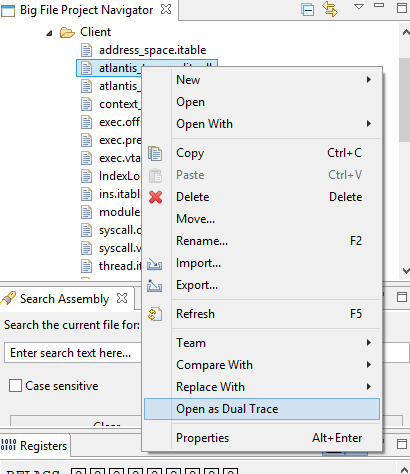
\includegraphics[scale=0.4]{Figures/opendualtracemenu}}
%DIFDELCMD <  %%%
\DIFdelendFL \DIFaddbeginFL \centerline{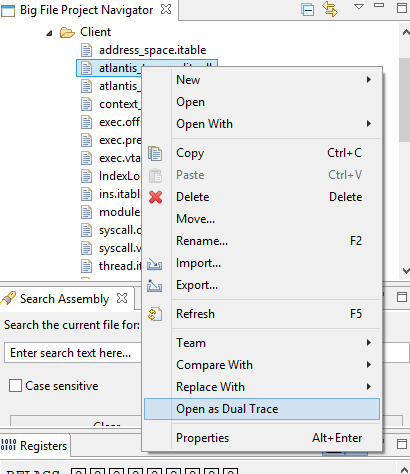
\includegraphics[scale=0.7]{Figures/opendualtracemenu}}
 \DIFaddendFL \caption{Menu item for opening dual\_trace}
\label{opendualtracemenu}
\end{figure}

\begin{figure}[H]
\centerline{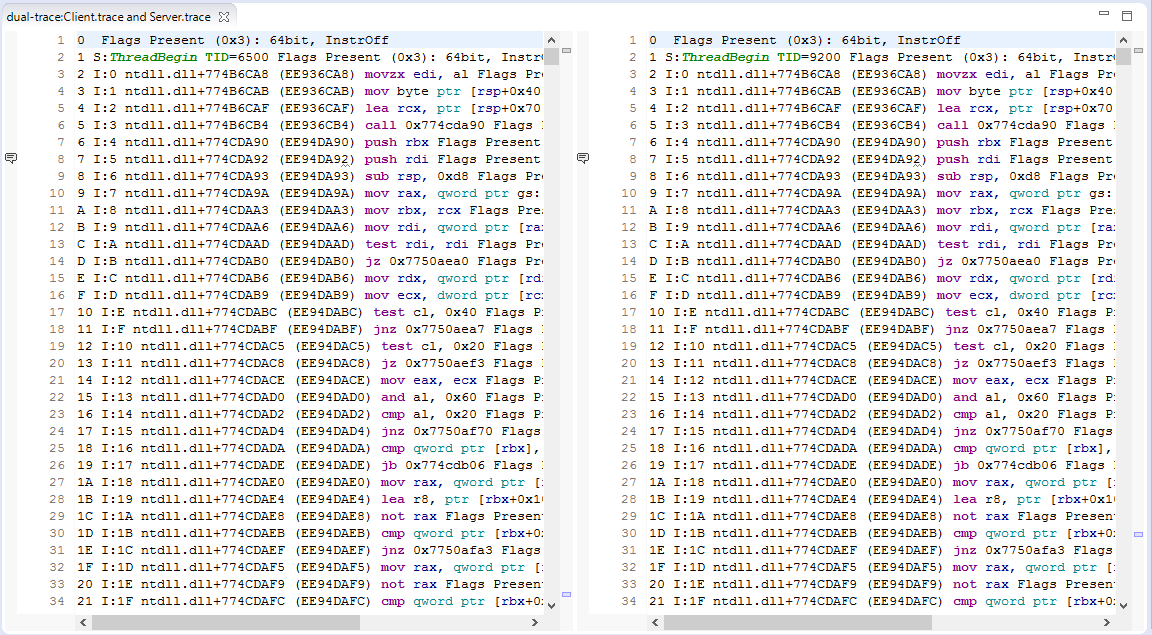
\includegraphics[scale=0.6]{Figures/paralleleditor}}
 \caption{Parallel trace view}
\label{parallelview}
\end{figure}

\section{Implementation of the Communication Analysis Algorithms}
The implementation is divided into two parts. The first part is the stream extraction. It implements the first section of the overall process of the communication analysis as shown in the left side of Figure \ref{overviewintwo} and presents the extracted streams of both traces in the dual\_trace to the user. The second part is the communication identification. It implements the whole process of the communication analysis as shown in the right side of Figure \ref{overviewintwo} and presents the identified communications of the dual\_trace to the user.

\begin{figure}[H]
\centerline{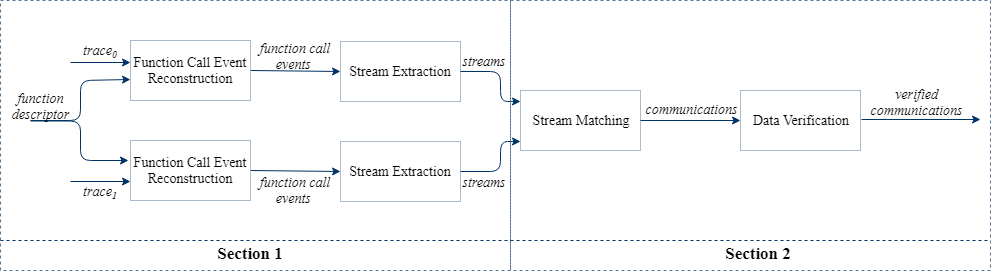
\includegraphics[scale=0.47]{Figures/overviewintwo}}
\caption{Process of the communication analysis from a dual\_trace separated in two sections}
\label{overviewintwo}
\end{figure}

The format of the traces I got from DRDC for this research is slightly different from the formulation of the trace in Section \ref{dualtrace}. Instead of having the function name in $syscallInfo$, the current traces only provide the offset of that function in the corresponding executable file. So, the trace needs to be processed to comply with the trace formalization.
The existing ``function inspect" feature of Atlantis can provide this pre-processing functionality. The called functions' names can be inspected by searching for the symbolic name in the executable binary or any DLLs used by the program at the time when it is traced. Figure \ref{trace} shows an example of the trace from DRDC. In this example, line 1504 is a system call entry with the system call information as $syscallInfo = <kernel32.dll, 0x10D10>$. 
Figure \ref{executable} is the information decoded by the ``function inspect" feature of Atlantis from the executable file kernel32.dll of the system where the trace shown in Figure \ref{trace} was captured. The instruction line 1504 is a system call entry of $CreateFileW$. By loading a .dll file (in this case kernel32.dll) for the trace, Atlantis can translate system call information in the current trace format to the one align to the dual\_trace formalization.

\begin{figure}[H]
\DIFdelbeginFL %DIFDELCMD < \centerline{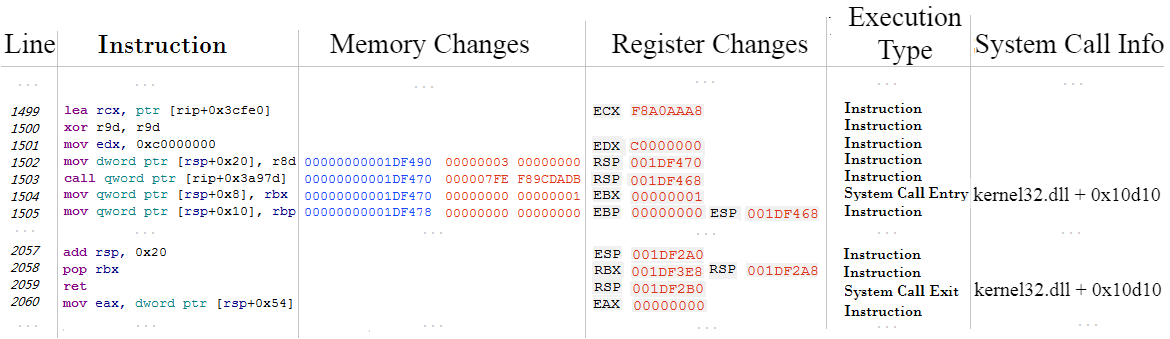
\includegraphics[scale=0.45]{Figures/trace}}
%DIFDELCMD < %%%
\DIFdelendFL \DIFaddbeginFL \centerline{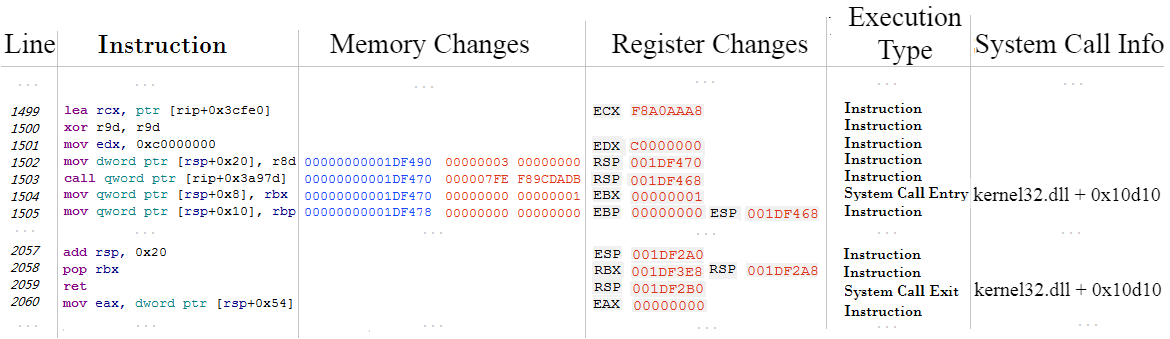
\includegraphics[scale=0.55]{Figures/trace}}
\DIFaddendFL \caption{An example trace from DRDC}
\label{trace}
\end{figure}

\begin{figure}[H]
\DIFdelbeginFL %DIFDELCMD < \centerline{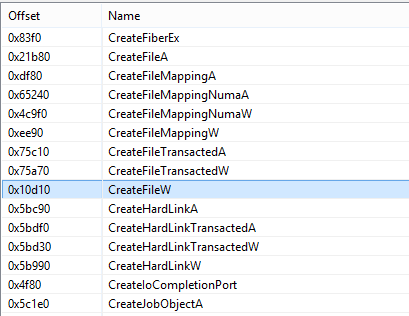
\includegraphics[scale=0.6]{Figures/executable}}
%DIFDELCMD < %%%
\DIFdelendFL \DIFaddbeginFL \centerline{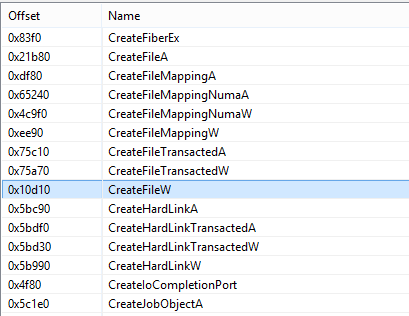
\includegraphics{Figures/executable}}
\DIFaddendFL \caption{Information from kernel32.dll}
\label{executable}
\end{figure}

A new menu ``Dual\_trace Tool" with three menu options is designed for these two operations. In this menu, ``Stream Extraction" is for the operation of stream extraction and ``Communication Identification" is for the operation of communication identification. Before performing both of these two operation, The ``Load Library Exports" has to be run for both traces. ``Load Library Exports" option in this menu triggers the ``function inspect" operation for the active trace. After this operation is run separately for both traces in the dual\_trace, the traces are transformed into the proper format for communication analysis. Figure \ref{dualtracetoolmenu} shows this new menu in Atlantis. When the user performs the ``Stream Extraction" or ``Communication Identification" operations, there will be a prompt dialog window as shown in Figure \ref{methods} which asks the user what communication methods they want to analyze from the dual\_trace. This list is provided by the configuration file I mentioned in Section \ref{functionset}. The user can select one or multiple methods. Atlantis will perform the operations after the user selects and confirms the communication methods.

\begin{figure}[H]
\centerline{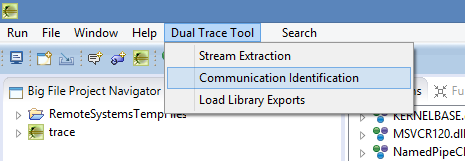
\includegraphics{Figures/dualtracetoolmenu}}
 \caption{Dual\_trace tool menu}
\label{dualtracetoolmenu}
\end{figure}

\begin{figure}[H]
\centerline{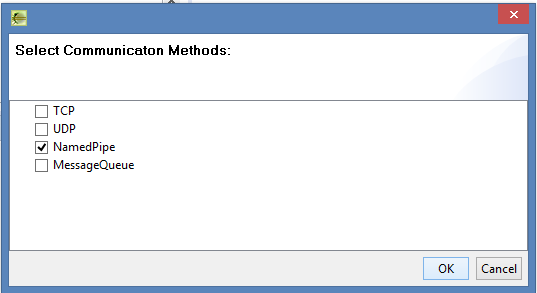
\includegraphics[scale=0.8]{Figures/methods}}
 \caption{Prompt dialog for communication selection}
\label{methods}
\end{figure}


\section{View of Extracted Streams and Identified Communications}
I designed a new view named ``Communication View" for presenting the result of the extracted streams and the identified communications. Since the user might have selected multiple selection for communication methods of interest, the output results contain all the streams or communications of all selected communication methods and the results are clustered by methods. There are two sub tables in this view, the left one is for presenting the extracted streams while the left one is for presenting identified communications. The reason for putting these two results in the same view is for easy access to and comparison of the data for the users. Figure \ref{idenview} shows this view with both extracted stream results and identified communication results in it. Each time when the user reruns the operations the result in the corresponding table will be refreshed to show only the latest result of that operation. But the other table will not be affected. For example, if the user runs the ``Stream Extraction" operation first, the extracted streams will be shown on the left table of the view. And then if the user performs the ``\DIFdelbegin \DIFdel{communication }\DIFdelend \DIFaddbegin \DIFadd{Communication }\DIFaddend Identification" operation, the identified communications result will be shown on the right table, while the left one still holds the last stream extraction result.

\begin{figure}[H]
\DIFdelbeginFL %DIFDELCMD < \centerline{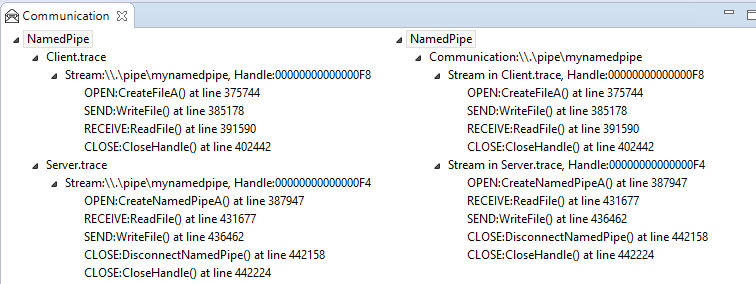
\includegraphics[scale=0.7]{Figures/idenview}}
%DIFDELCMD <  %%%
\DIFdelendFL \DIFaddbeginFL \centerline{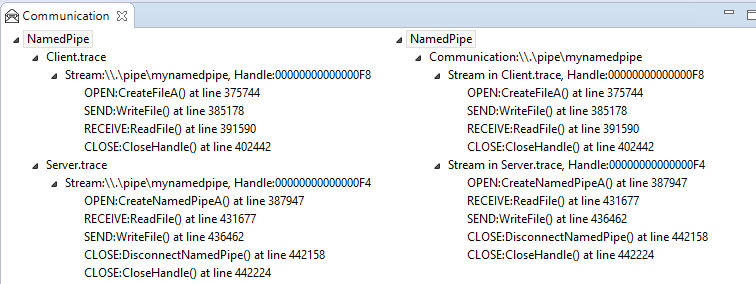
\includegraphics[scale=0.8]{Figures/idenview}}
 \DIFaddendFL \caption{Communication view for results}
\label{idenview}
\end{figure}

Atlantis is an analysis environment that has various views to provide user access to different information from a trace, such as the memory and register state of the current instruction line. Moreover, these views synchronize automatically with the trace view. This functionality and information also benefits the communication analysis of the dual\_trace. Providing the user a way to navigate from the result of the extracted streams and the identified communications to the trace view allows them to take advantage of the current existing functionality of Atlantis and make their analysis of the dual\_trace more efficient.

The results presented in the Communication view contains all the function call events. The memory state at the instruction line of the function begin contains the input parameters and the memory state at the instruction line of the function return contains the output parameters and the return value. In order to provide the user a method to easily access these two instruction lines, from the event entries, this implementation provides two different ways for the user to navigate back to where the function begins and ends. When the user ``double clicks" on an entry, it will bring the user to the start line of the function in the corresponding trace view. When the user right clicks on the event entry, a prompted menu with the option ``Go To Line of Function End" will show up as shown in Figure \ref{gotoend}. Clicking on this option will bring the user to the return line of this function in the trace view. All other opened views of Atlantis update immediately with this navigation. By these navigations, the users can easily see the sent and received message of the events.

\begin{figure}[H]
\centerline{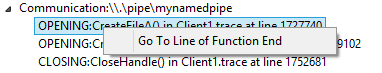
\includegraphics{Figures/gotoend}}
 \caption{Right click menu on event entry}
\label{gotoend}
\end{figure}

Moreover, the ``remove" option, as shown in Figure \ref{remove}, in the right click menu on the ``stream“ or ``communication" entries is provided for the user to remove the selected ``stream" or ``communication" entry. This provides the users the flexibility to get rid of data that they are not interested about.

\begin{figure}[H]
\centerline{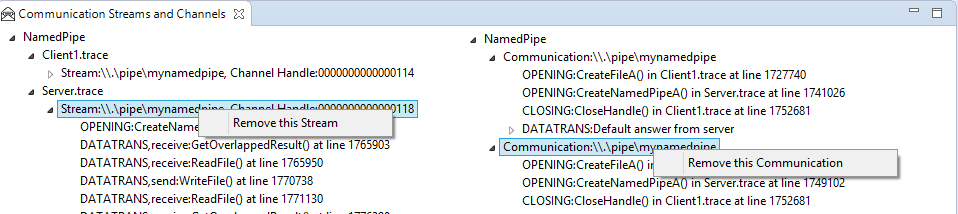
\includegraphics[scale=0.7]{Figures/remove}}
 \caption{Right click menu on event entry}
\label{remove}
\end{figure}


	\externaldocument{../appendix/chapter_app}
\externaldocument{../4/chapter_algorithm}
\externaldocument{../3/chapter_modeling}
\startchapter{Proof of Concept}
\label{chapter:Exp}
In this chapter, I present two experiments I ran as a proof of concept of the communication analysis of dual\_trace.

These experiments were aimed to test the communication model and the communication analysis approach. They also verify the correctness of the algorithms. I used the implemented features on Atlantis to conduct the experiments.

The selection of the experiments are restricted by the traces that can be captured. The current in-house tracer of DRDC is only able to capture the function information for some .dll files. kernel32.dll which contains the functions for Named Pipe is one of the .dll files that this tracer can capture. Functions for the other communication methods discussed in this thesis can not be captured by DRDC's tracer currently.  Thus both of the conducted experiments used the Named Pipe communication method. 

Among these two experiments, the first one was provided directly by our research partner DRDC with their initial requirement, while I designed the second one. In both experiments, DRDC conducted the programs execution and captured the traces on their environment, while I performed the analysis locally with Atlantis on my desktop with the captured traces. All test programs in these two experiments were written in C++ and the source code can be found in Appendix \ref{expcode}. 

In both experiments, three major steps are conducted:
\begin{enumerate}
\item Execute the test programs and capture the traces for each program (done by DRDC)

\item Perform the ``Stream Exaction" and ``Communication Identification" operation on the dual\_trace

\item Manually verify the results by navigating the events in the ``Communication view" and check if they match the sequence diagrams of each experiment
\end{enumerate}

In the following two sections, I describe the design of the experiments first and then present the results of them with discussion of each one.

\section{Experiment 1}
\subsection{Experiment Design}
In the first experiment, two programs communicated with each other through a synchronous named pipe channel. One of the programs acted as the named pipe server while the other as the client. Figure \ref{exp1} is the sequence diagram of the interaction between the server and client. This sequence diagram only exemplifies a possible sequence of the events. The actual event sequence can vary depending on the run-time environment. 


\begin{figure}[H]
\centerline{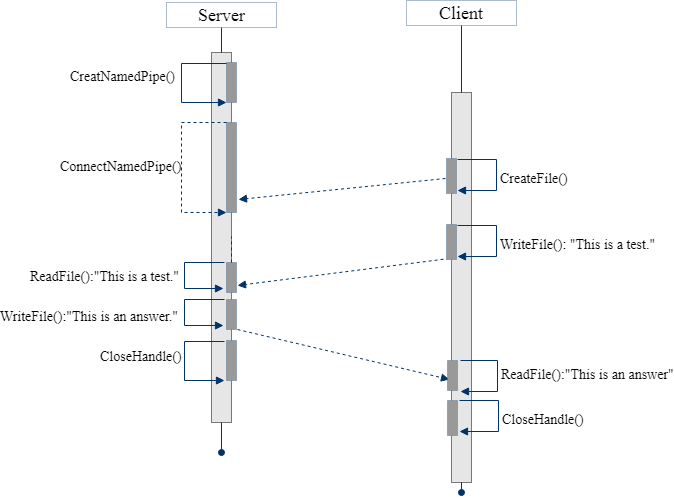
\includegraphics[scale=0.6]{Figures/exp1}}
 \caption{Sequence diagram of experiment 1}
\label{exp1}
\end{figure}

The traces of these programs running and interacting were captured. The two captured traces, $Sever.trace$ and $Client.trace$ were analyzed as a dual\_trace and named $dual\_trace\_1$. I performed ``Stream identification" and ``Communication identification" following the use cases in Table \ref{usecase1} and Table \ref{usecase2} with $dual\_trace\_1$ and the corresponding kernel32.dll. The functions descriptor for the analysis of $dual\_trace\_1$ is shown in Table \ref{fdescexp1}.

\begin{table}[H]
  \centering
  \caption{Functions descriptor of Named Pipe for experiment 1}
  \label{fdescexp1}
  \begin{tabular}{|l|l|l|l|l|l|l|l|}
\hline
             \multirow{2}{*}{{\textbf{Name}}} & \multirow{2}{*}{{\textbf{Type}}} & \multicolumn{3}{c|}{\textbf{Input Parameters Description}} & \multicolumn{3}{c|}{\textbf{Output Parameters Description}} \\
              \cline{3-8} 
             & & \textbf{Name}& \textbf{Register} & \textbf{Addr/Val} & \textbf{Name}& \textbf{Register} &  \textbf{Addr/Val}  \\
             \hline
      CreateNamedPipeA
       &open & FileName & RCX  & Addr &  Handle & RAX & Val\\
      \hline         
      CreateFileA
       &open & FileName & RCX & Addr&  Handle & RAX & Val\\ 
      \hline              
      \multirow{2}{*}{WriteFile}
       &\multirow{2}{*}{send} &  Handle & RCX & Val & Length& R9 &Val\\
        \cline{3-8} 
       & & SendBuf & RDX & Addr & RetVal& RAX & Val\\
      \hline            
      \multirow{2}{*}{ReadFile}
       &\multirow{2}{*}{receive} &  Handle & RCX & Val& Length &R9 & Val\\
        \cline{3-8} 
       & & RecvBuf & RDX  & Addr & RetVal& RAX & Val\\
      \hline            
      CloseHandle &
       close &  Handle & RCX & Val & RetVal& RAX & Val\\
      \hline            
      DisconnectNamedPipe &
      close &  Handle & RCX & Val & RetVal& RAX & Val\\
      \hline               
  \end{tabular}
\end{table}


\subsection{Dual\_trace Analysis Results Walk Through}
$Client.trace$ has 412,717 instruction lines. Four function call events were reconstructed from this trace as listed in Table \ref{funcclientexp1}.

\begin{table}[H]
  \centering
  \tiny
  \caption{The sequence of function call events of $Client.trace$}
  \label{funcclientexp1}
  \begin{tabular}{|l|p{16cm}|}
  \hline
\textbf{Line} & \multicolumn{1}{>{\centering\arraybackslash}m{16cm}|}{\textbf{Event}}\\
  \hline
  375744 & $funN:CreateFileA,  type:open, inparams:\lbrace Handle:0xF8, FileName:``.\backslash pipe \backslash mynamepipe" \rbrace, outparams:\lbrace RetVal:0 \rbrace$\\
 \hline
  385178 & $funN:WriteFile, type:send, inparams:\lbrace Handle:0xF8, SendBuf:``This\; is\; a\; test."\rbrace, outparams: \lbrace Length:15 \rbrace$\\
\hline
 391590&$funN:ReadFile, type:receive, inparams: \lbrace Handle:0xF8 \rbrace, outparams: \lbrace RecvBuf:``This\; is\; the\; answer.", Length:18, RetVal:0 \rbrace$\\
\hline
 402442&$funN:CloseHandle, type:close, inparams: \lbrace Handle:0xF8 \rbrace, outparams: \lbrace RetVal:0 \rbrace$\\
\hline               
  \end{tabular}
\end{table}

The values of the handle parameter of these four events are $0xF8$. So a stream was extracted, which consists of all these four function call events. 

$Server.trace$ has 461,817 instruction lines. Five function call events were reconstructed from this trace as listed in Table \ref{funcserverexp1}.

\begin{table}[H]
  \centering
  \tiny
  \caption{The sequence of function call events of $Server.trace$}
  \label{funcserverexp1}
  \begin{tabular}{|l|p{16cm}|}
  \hline
\textbf{Line} & \multicolumn{1}{>{\centering\arraybackslash}m{16cm}|}{\textbf{Event}}\\
  \hline
  387947 & $funN:CreateNamedPipeA,  type:open, inparams:\lbrace Handle:0xF4, FileName:``.\backslash pipe \backslash mynamepipe" \rbrace, outparams:\lbrace RetVal:0 \rbrace$\\
 \hline
  431677&$funN:ReadFile, type:receive, inparams: \lbrace Handle:0xF4 \rbrace, outparams: \lbrace RecvBuf:``This\; is\; a\; test.", Length:15, RetVal:0 \rbrace$\\
\hline
  436462 & $funN:WriteFile, type:send, inparams:\lbrace Handle:0xF4, SendBuf:``This\; is\; the\; answer."\rbrace, outparams: \lbrace Length:18 \rbrace$\\
\hline
 442158&$funN:DisconnectNamedPipe, type:close, inparams: \lbrace Handle:0xF4 \rbrace, outparams: \lbrace RetVal:0 \rbrace$\\
\hline   
 442224&$funN:CloseHandle, type:close, inparams: \lbrace Handle:0xF4 \rbrace, outparams: \lbrace RetVal:0 \rbrace$\\
\hline               
  \end{tabular}
\end{table}

The values of the handle parameter of these five events are $0xF4$. So, a stream was extracted, which consists of all of these five function call events. 

The extracted streams were listed in the left table of the ``Communication view"  as shown in Figure \ref{result1_streams}.

\begin{figure}[H]
\centerline{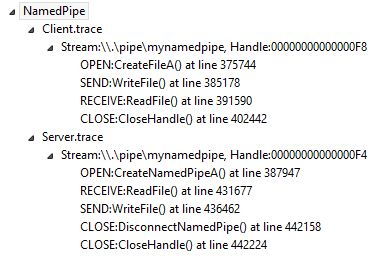
\includegraphics{Figures/result1_streams}}
 \caption{Extracted streams of $dual\_trace\_1$}
\label{result1_streams}
\end{figure}

The value of the $FileName$ parameter of the $CreateFileA$ function call event in $Client.trace$ is $``.\backslash pipe \backslash mynamepipe"$ as shown in Table \ref{funcclientexp1}. Meanwhile, the value of the $FileName$ parameter of the $CreateNamePipeA$ function call event in $Server.trace$ is also $``.\backslash pipe \backslash mynamepipe"$ as shown in Table \ref{funcserverexp1}. According to the algorithm presented in Section \ref{streammatch}, the file name of a named pipe is treated as the channel identifier which is used to match two streams into a communication. So the stream in $Client.trace$ is matched to the stream identified by the $0xF4$ in $Server.trace$.

There is only one send event and one receive event in both streams, the data verification of these two matched streams is trivial. Both the concatenation of the sent packet(s) in the stream $0xF8$ of $Client.trace$ and the concatenation of the received packet(s) in the stream $0xF4$ of $Server.trace$ are $``This\; is\; a\; test."$. Both the concatenation of the sent packet(s) in the stream $0xF4$ of $Server.trace$ and the concatenation of the received packet(s) in the stream $0xF8$ of $Client.trace$ are $``This\; is\; the\; answer."$. So these two match streams satisfy the content preservation of the reliable communication. Therefore, they are eventually output as a communication by the ``Communication Identification" operation and listed in the right table of the ``Communication view" in Atlantis as shown in Figure \ref{result1_communications}.


\begin{figure}[H]
\centerline{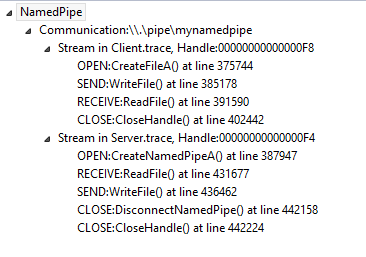
\includegraphics{Figures/result1_communications}}
 \caption{Identified communication of $dual\_trace\_1$}
\label{result1_communications}
\end{figure}


After seeing the identified communication from $dual\_trace\_1$, I navigated from the send event entries via ``double click" and receive event entries via ``Go To Line of Function End" to the traces. The navigation results are shown in Figures \ref{result1_client_to_server} and \ref{result1_server_to_client}.

\DIFdelbegin %DIFDELCMD < \begin{figure}[H]
%DIFDELCMD < \begin{subfigure}[H]{0.45\linewidth}
%DIFDELCMD < 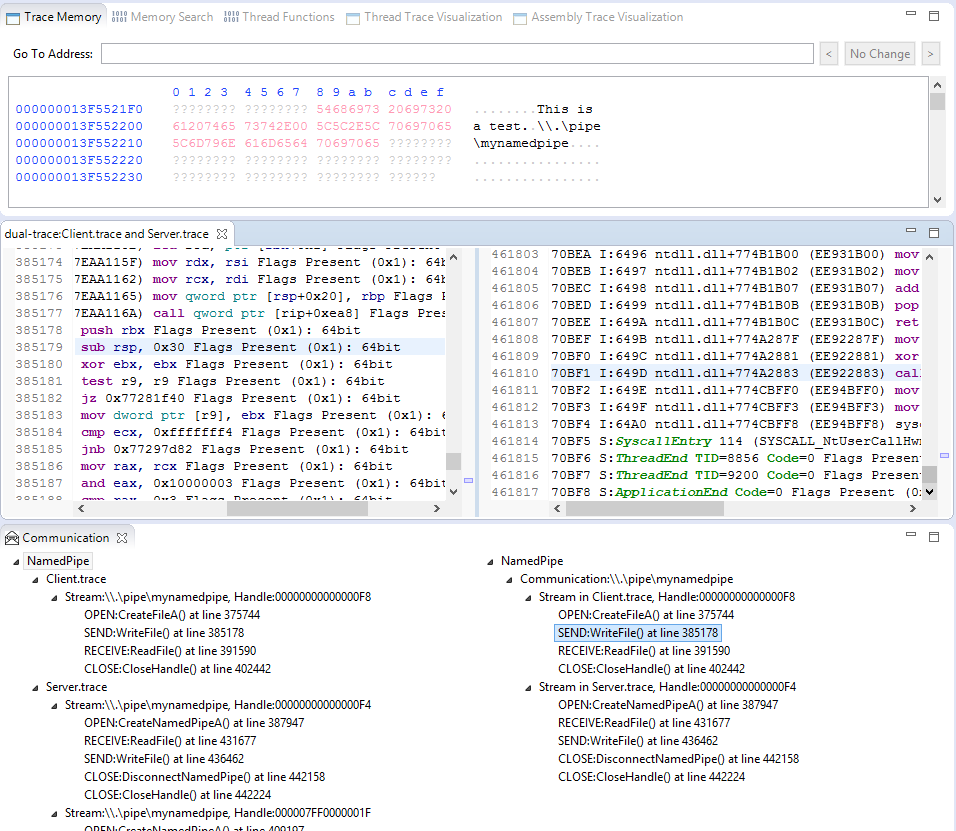
\includegraphics[scale=0.35]{Figures/result1_client_send}
%DIFDELCMD <  %%%
\DIFdelendFL \DIFaddbeginFL \begin{figure}
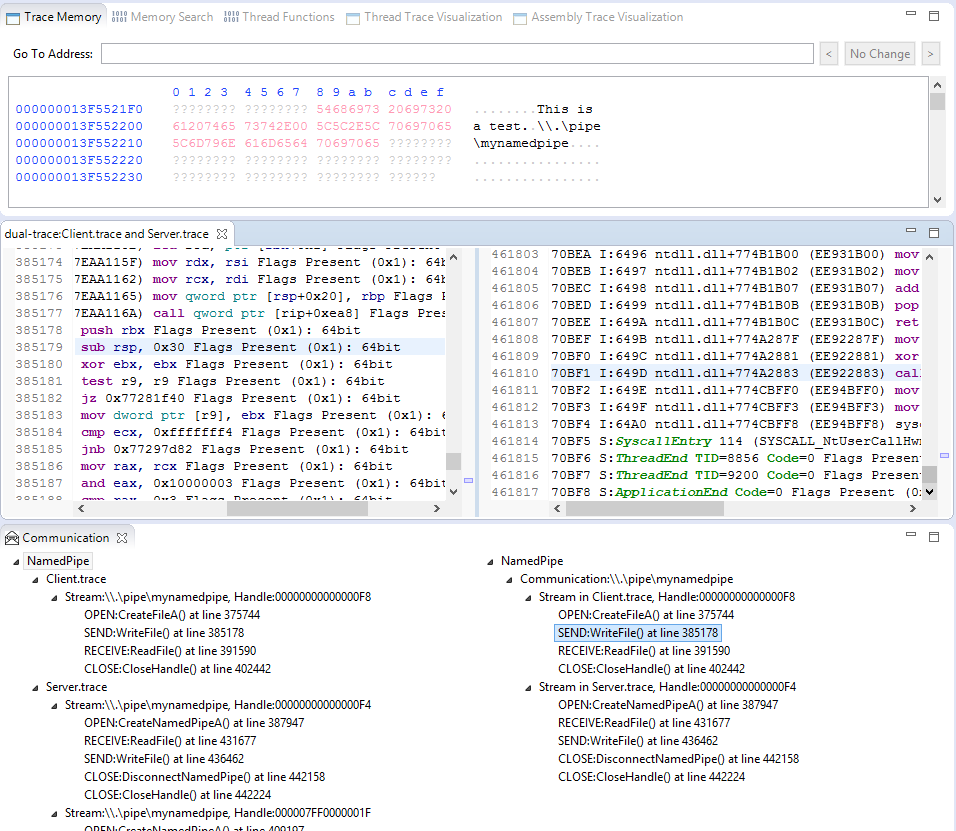
\includegraphics[scale=0.7]{Figures/result1_client_send}
 \DIFaddendFL \caption{Client send event navigation \DIFaddbeginFL \DIFaddFL{for the message $``This\; is\; a\; test."$}\DIFaddendFL }
\label{result1_client_send}
\DIFdelbeginFL %DIFDELCMD < \end{subfigure}
%DIFDELCMD < \hfill
%DIFDELCMD < \begin{subfigure}[H]{0.45\linewidth}
%DIFDELCMD < 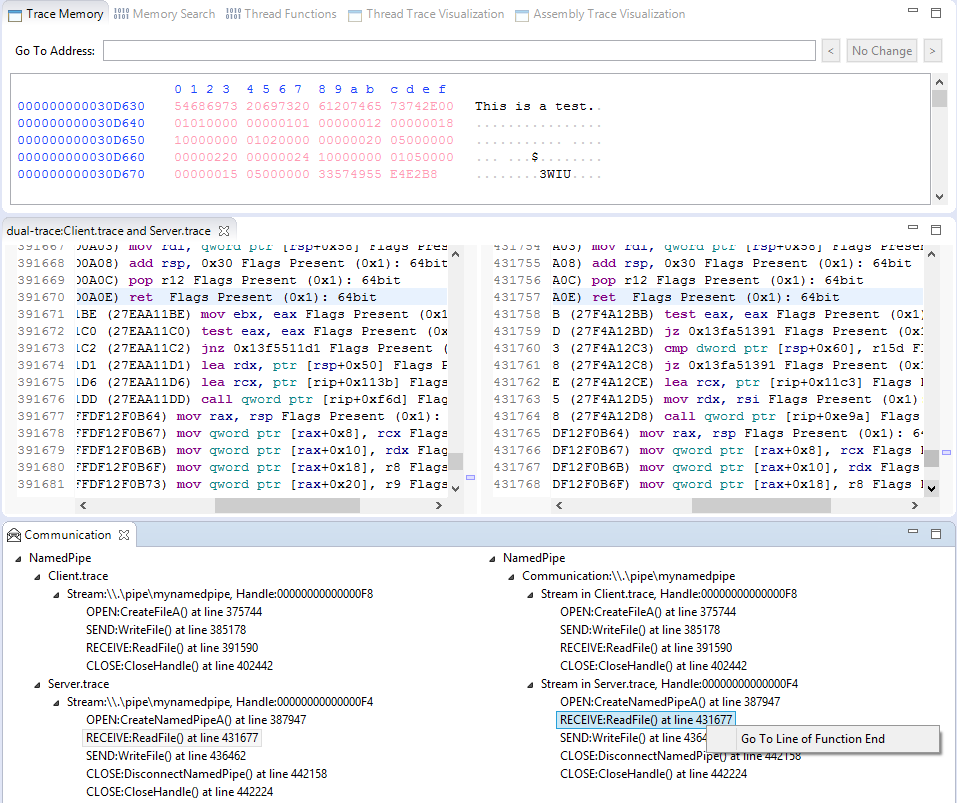
\includegraphics[scale=0.35]{Figures/result1_server_read}
%DIFDELCMD <  %%%
\DIFdelendFL \DIFaddbeginFL \end{figure}

\begin{figure}
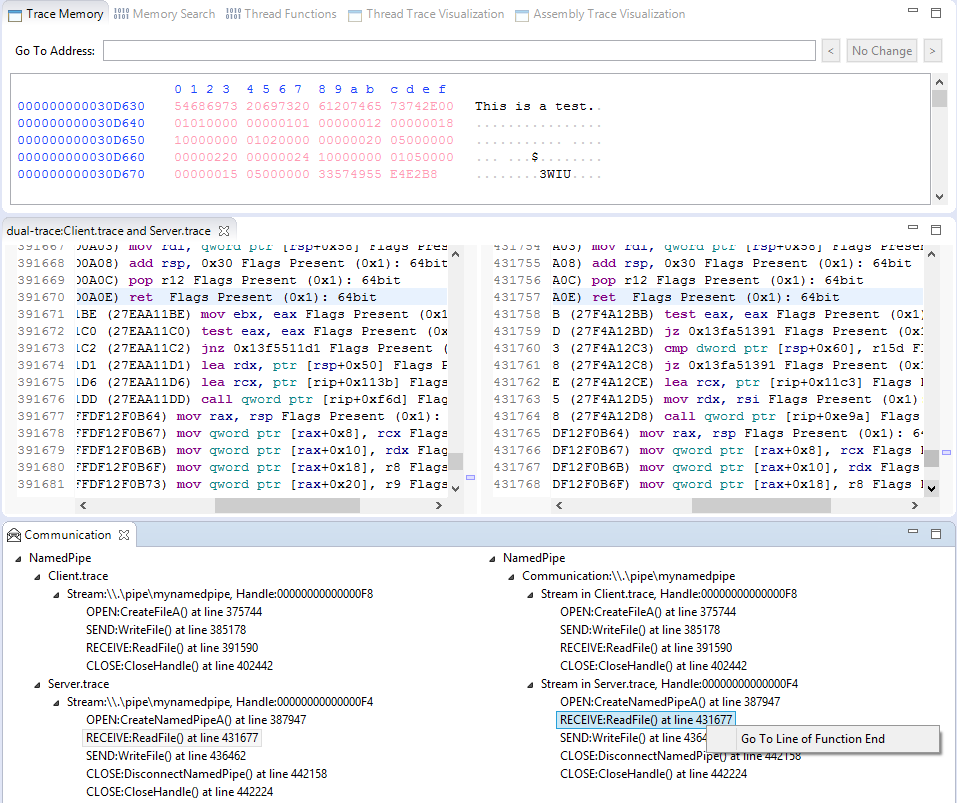
\includegraphics[scale=0.7]{Figures/result1_server_read}
 \DIFaddendFL \caption{Server receive event navigation \DIFaddbeginFL \DIFaddFL{for the message $``This\; is\; a\; test."$}\DIFaddendFL }
\label{result1_server_read}
\DIFdelbeginFL %DIFDELCMD < \end{subfigure}%%%
%DIF < 
%DIFDELCMD < \caption{%
{%DIFAUXCMD
\DIFdelFL{Navigation results for the transmitted message $``This\; is\; a\; test."$}}
%DIFAUXCMD
%DIFDELCMD < \label{result1_client_to_server}
%DIFDELCMD < %%%
\DIFdelendFL \end{figure}

Figure \ref{result1_client_send} shows when I double clicked on the $WriteFile$ function call event of the $Client.trace$, it brought me to the ``Trace view" of the $Client.trace$ on line 385178 where the function started, and the ``Trace Memory view" jumped to the memory address $0x13F5521F8$, which is the address for the send buffer of the message $``This\; is\; a\; test."$.

Figure \ref{result1_server_read} shows when I selected ``Go To Line of Function End" from the right click menu on the $ReadFile$ function call event of $Server.trace$, that it brought me to the ``Trace view" of $Server.trace$ on line 431757 where the function returned, and the ``Trace Memory view" jumped to the memory address $0x30D630$, which is the address for the receive buffer of the message $``This\; is\; a\; test."$.

These two figures show how the message $``This\; is\; a\; test."$ is transmitted from the client to the server.

\DIFdelbegin %DIFDELCMD < \begin{figure}[H]
%DIFDELCMD < \begin{subfigure}[H]{0.45\linewidth}
%DIFDELCMD < 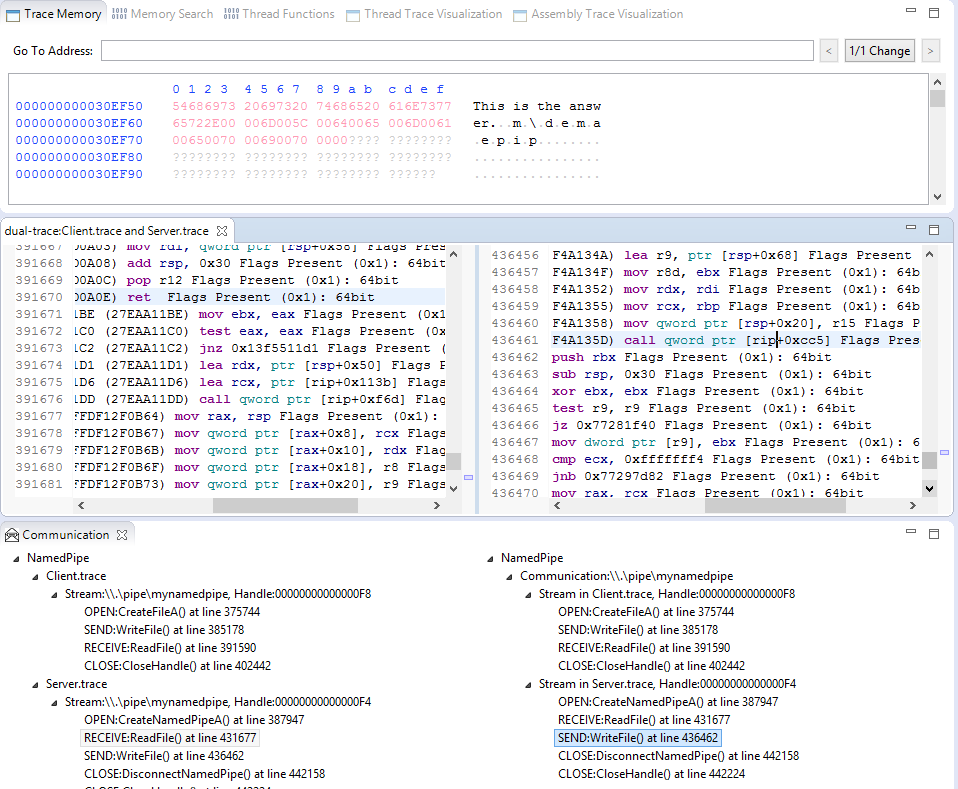
\includegraphics[scale=0.35]{Figures/result1_server_send}
%DIFDELCMD <  %%%
\DIFdelendFL \DIFaddbeginFL \begin{figure}
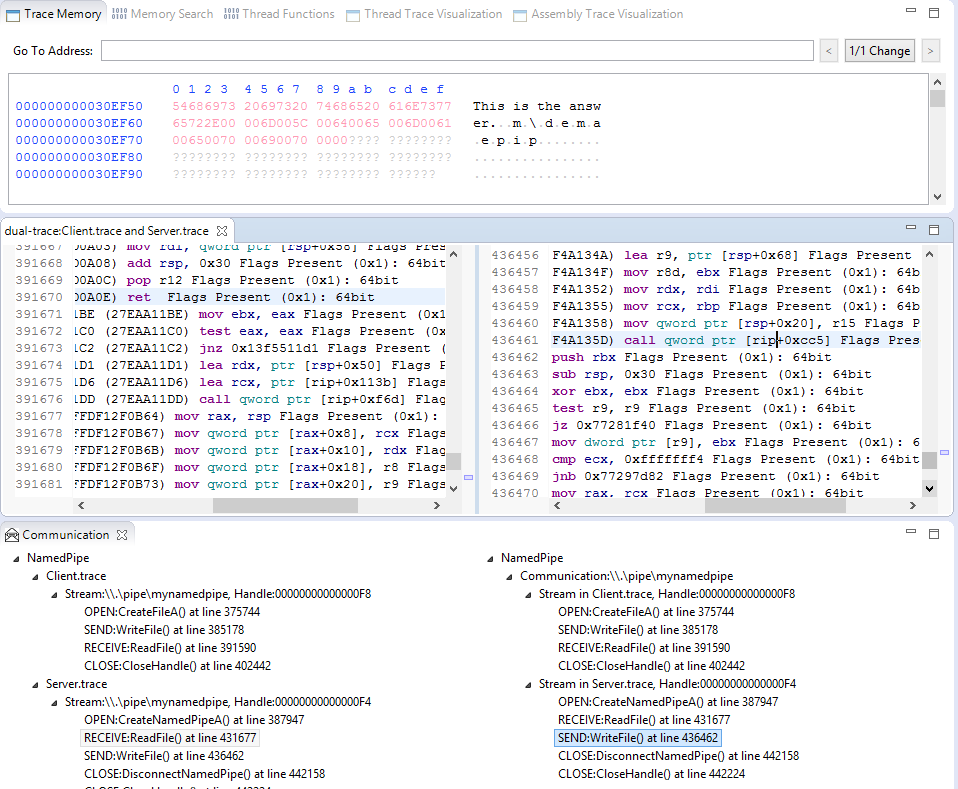
\includegraphics[scale=0.7]{Figures/result1_server_send}
 \DIFaddendFL \caption{Server send event navigation \DIFaddbeginFL \DIFaddFL{for the message $``This\; is\; the\; answer."$}\DIFaddendFL }
\label{result1_server_send}
\DIFdelbeginFL %DIFDELCMD < \end{subfigure}
%DIFDELCMD < \hfill
%DIFDELCMD < \begin{subfigure}[H]{0.45\linewidth}
%DIFDELCMD < 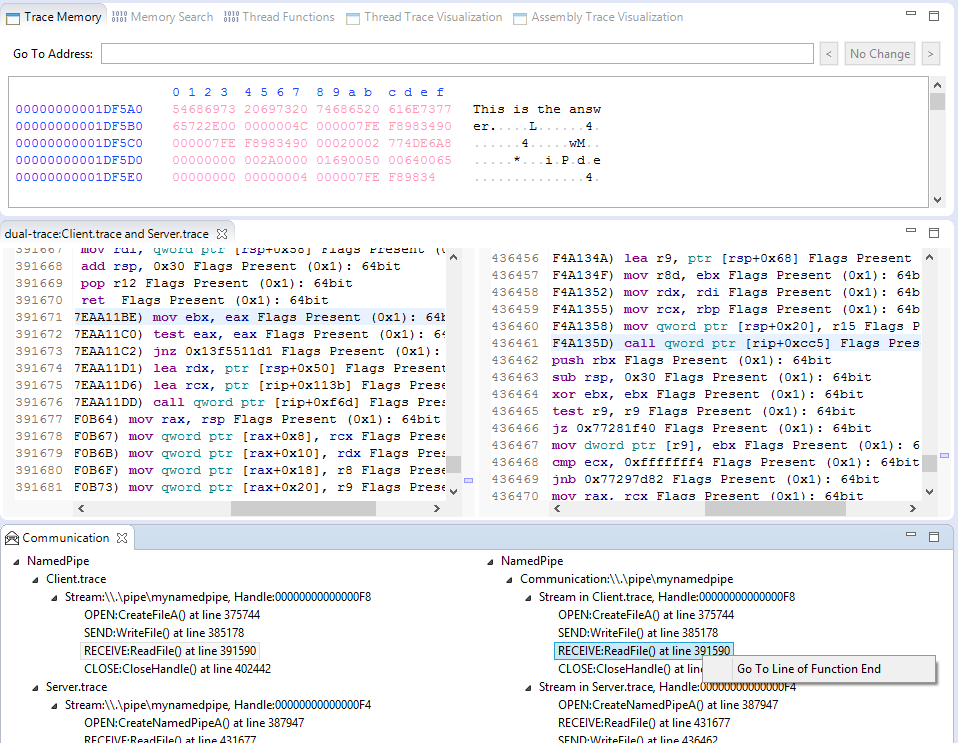
\includegraphics[scale=0.35]{Figures/result1_client_read}
%DIFDELCMD <  %%%
\DIFdelendFL \DIFaddbeginFL \end{figure}

\begin{figure}
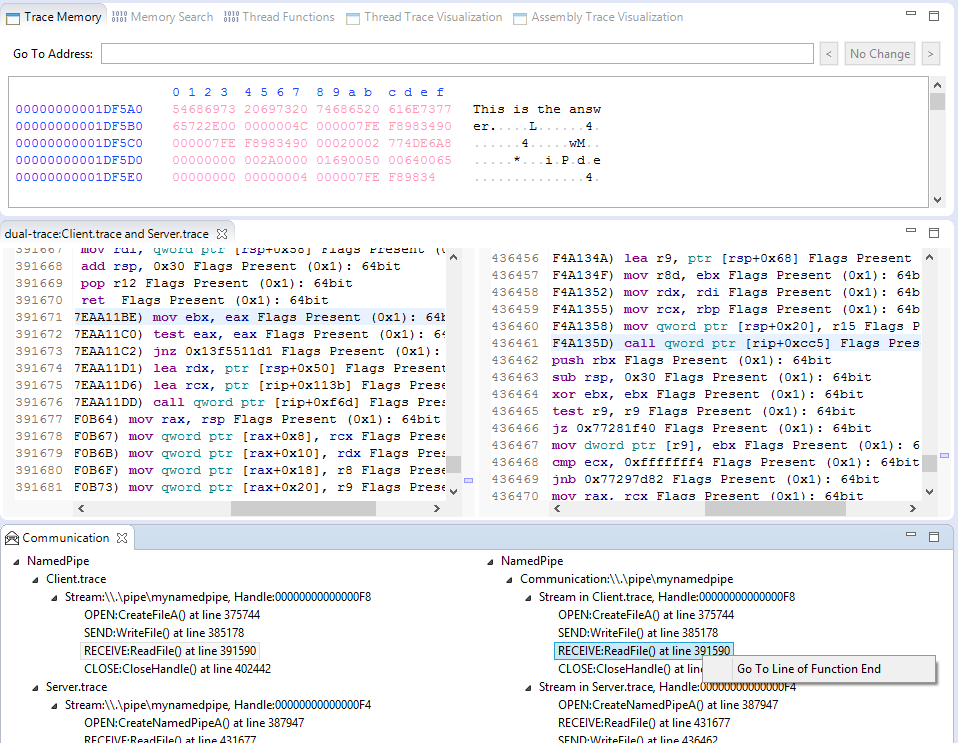
\includegraphics[scale=0.7]{Figures/result1_client_read}
 \DIFaddendFL \caption{Client receive event navigation \DIFaddbeginFL \DIFaddFL{for the message $``This\; is\; the\; answer."$}\DIFaddendFL }
\label{result1_client_read}
\DIFdelbeginFL %DIFDELCMD < \end{subfigure}%%%
%DIF < 
%DIFDELCMD < \caption{%
{%DIFAUXCMD
\DIFdelFL{Navigation results for the transmitted message $``This\; is\; the\; answer."$}}
%DIFAUXCMD
%DIFDELCMD < \label{result1_server_to_client}
%DIFDELCMD < %%%
\DIFdelendFL \end{figure}

Figure \ref{result1_server_send} shows when I double clicked on the $WriteFile$ function call event of $Server.trace$, it brought me to the ``Trace view" of $Server.trace$ on line 436462 where the function started, and the ``Trace Memory view" jumped to the memory address $0x30EF50$, which is the address for the send buffer of the message $``This\; is\; the\; answer."$.

Figure \ref{result1_client_read} shows when I selected ``Go To Line of Function End" in the right click menu on the $ReadFile$ function call event of the $Client.trace$, it brought me to the ``Trace view" of the $Client.trace$ on line 391670 where the function returned, and the ``Trace Memory view" jumped to the memory address $0x1DF5A0$, which is the address for the receive buffer of the message $``This\; is\; the\; answer."$.

These two figures perfectly show how the message $``This\; is\; the\; answer."$ is transmitted from the server to the client.

\section{Experiment 2}
\subsection{Experiment Design}
In the second experiment, one server program and one client program are written in C++. In the server program, four named pipes were created and could be connected by up to four clients at a time. The named pipe client program was run two times in sequence to act as two clients, client1 and client2. Both of these two clients actually connected to the server but sent different messages. Figure \ref{exp2} is the sequence diagram of the interaction among the server and the two clients. This sequence diagram only exemplifies a possible sequence of the events. The actual events sequence can vary depending on the run-time environment. 

Three traces were captured when these three programs were running and interacting with each other. They are $Server.trace$ for the program execution of server , $Client1.trace$ for the program execution of Client 1 and $Client2.trace$ for the program execution of Client 2. These three traces were analyzed as two dual\_traces. The one consisting of $Server.trace$ and $Client1.trace$ is named $dual\_trace\_21$. The other consisting of $Server.trace$ and $Client2.trace$ is named $dual\_trace\_22$. I performed the ``Stream Extraction" and ``Communication Identification" operations for these two dual\_traces with the functions descriptor in Table \ref{fdescexp2}.

\begin{figure}[H]
\centerline{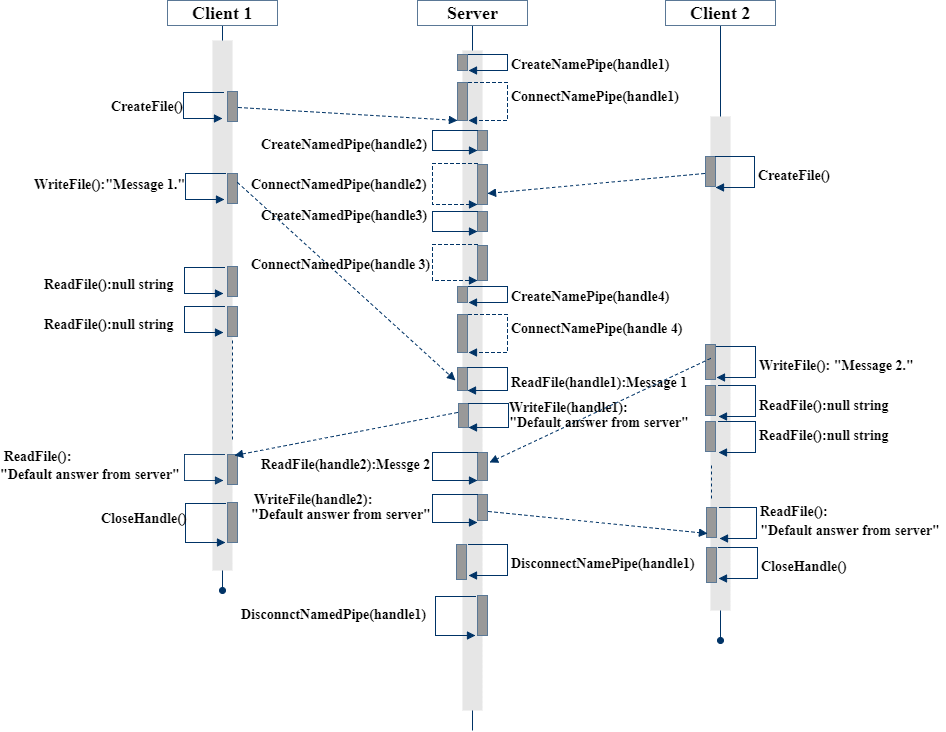
\includegraphics[scale=0.55]{Figures/exp2}}
 \caption{Sequence diagram of experiment 2}
\label{exp2}
\end{figure}


\begin{table}[H]
  \centering
  \caption{Functions descriptor of Named Pipe for experiment 2}
  \label{fdescexp2}
\begin{tabular}{|l|l|l|l|l|l|l|l|}
\hline
             \multirow{2}{*}{{\textbf{Name}}} & \multirow{2}{*}{{\textbf{Type}}} & \multicolumn{3}{c|}{\textbf{Input Parameters Description}} & \multicolumn{3}{c|}{\textbf{Output Parameters Description}} \\
              \cline{3-8} 
             & & \textbf{Name}& \textbf{Register} & \textbf{Addr/Val} & \textbf{Name}& \textbf{Register} &  \textbf{Addr/Val}  \\
             \hline
      CreateNamedPipe
       &open & FileName & RCX  & Addr &  Handle & RAX & Val\\
      \hline         
      CreateFile
       &open & FileName & RCX & Addr&  Handle & RAX & Val\\ 
      \hline              
      \multirow{2}{*}{WriteFile}
       &\multirow{2}{*}{send} &  Handle & RCX & Val & Length & R9 & Val\\
        \cline{3-8} 
       & & SendBuf & RDX & Addr & RetVal& RAX & Val\\
      \hline            
      \multirow{2}{*}{ReadFile}
       &\multirow{2}{*}{receive} &  Handle & RCX & Val& Length & R9 & Val\\
        \cline{3-8} 
       & & RecvBuf & RDX  & Addr & RetVal& RAX & Val\\
      \hline    
           \multirow{2}{*}{GetOverlappedResult} &
       \multirow{2}{*}{receive} &  \multirow{2}{*}{Handle} & \multirow{2}{*}{RCX} & \multirow{2}{*}{Val} &OverlapStruct &RDX & Addr\\
               \cline{6-8} 
       & &  &   &  & RetVal& RAX & Val\\
      \hline     
      CloseHandle &
       close &  Handle & RCX & Val & RetVal& RAX & Val\\
      \hline            
      DisconnectNamedPipe &
      close &  Handle & RCX & Val & RetVal& RAX & Val\\
      \hline               
  \end{tabular}  
\end{table} 

\subsection{Dual\_trace Analysis Results Walk Through}
In this section, I first walk through the function call event reconstruction and stream extraction results for each traces: $Server.trace$, $Client1.trace$ and $Client2.trace$. Then I walk through the communication identification results for each dual\_traces: $dual\_trace\_21$ and $dual\_trace\_22$.

\subsubsection{$\boldsymbol{Server.trace:}$}
$Server.trace$ has 1,789,627 instruction lines. Twelve function call events were reconstructed from this trace as listed in Table \ref{funcserverexp1}.

\begin{table}[H]
  \centering
  \tiny
  \caption{The sequence of function call events of $Server.trace$}
  \label{funcserverexp2}
  \begin{tabular}{|l|p{16cm}|}
  \hline
\textbf{Line} & \multicolumn{1}{>{\centering\arraybackslash}m{16cm}|}{\textbf{Event}}\\
  \hline
  1732413 & $funN:CreateNamedPipeA,  type:open, inparams:\lbrace Handle:0x118, FileName:``\dot \backslash pipe \backslash mynamepipe" \rbrace, outparams:\lbrace RetVal:0 \rbrace$\\
 \hline
   1741477 & $funN:CreateNamedPipeA,  type:open, inparams:\lbrace Handle:0x120, FileName:``\dot \backslash pipe \backslash mynamepipe" \rbrace, outparams:\lbrace RetVal:0 \rbrace$\\
 \hline
   1749553 & $funN:CreateNamedPipeA,  type:open, inparams:\lbrace Handle:0x128, FileName:``\dot \backslash pipe \backslash mynamepipe" \rbrace, outparams:\lbrace RetVal:0 \rbrace$\\
 \hline
   1757626 & $funN:CreateNamedPipeA,  type:open, inparams:\lbrace Handle:0x130, FileName:``\dot \backslash pipe \backslash mynamepipe" \rbrace, outparams:\lbrace RetVal:0 \rbrace$\\
 \hline
   1765903 & $funN:GetOverlappedResult, type:receive, inparams:\lbrace Handle:0x118 \rbrace, outparams: \lbrace OverlapStruct:``", RetVal:0\rbrace$\\
\hline
  1765950&$funN:ReadFile, type:receive, inparams: \lbrace Handle:0x118 \rbrace, outparams: \lbrace RecvBuf:``Message\: 2", Length:10, RetVal:0 \rbrace$\\
\hline
  1770738 & $funN:WriteFile, type:send, inparams:\lbrace Handle:0x118, SendBuf:``Default\: answer\: from\: server"\rbrace, outparams: \lbrace Length:20 \rbrace$\\
\hline
   1771629 & $funN:GetOverlappedResult, type:receive, inparams:\lbrace Handle:0x120 \rbrace, outparams: \lbrace OverlapStruct:``", RetVal:0\rbrace$\\
\hline
  1771676&$funN:ReadFile, type:receive, inparams: \lbrace Handle:0x120 \rbrace, outparams: \lbrace RecvBuf:``Message\: 1", Length:10, RetVal:0 \rbrace$\\
\hline
  1775507 & $funN:WriteFile, type:send, inparams:\lbrace Handle:0x120, SendBuf:``Default\: answer\: from\: server"\rbrace, outparams: \lbrace Length:20 \rbrace$\\
\hline
 1777180&$funN:DisconnectNamedPipe, type:close, inparams: \lbrace Handle:0x118 \rbrace, outparams: \lbrace RetVal:0 \rbrace$\\
\hline   
 1778658&$funN:DisconnectNamedPipe, type:close, inparams: \lbrace Handle:0x120 \rbrace, outparams: \lbrace RetVal:0 \rbrace$\\
\hline               
  \end{tabular}
\end{table}

There are four handle values in this event sequence: $0x118$, $0x120$, $0x128$, $0x130$. So four streams are extracted with these four handle identifiers. Both stream $0x118$ and $0x120$ have five events while stream $0x128$ and $0x130$ only have one channel open event. The extracted streams were listed in the left table  of ``Communication view"  as shown in Figure \ref{result21_streams}.

\begin{figure}[H]
\centerline{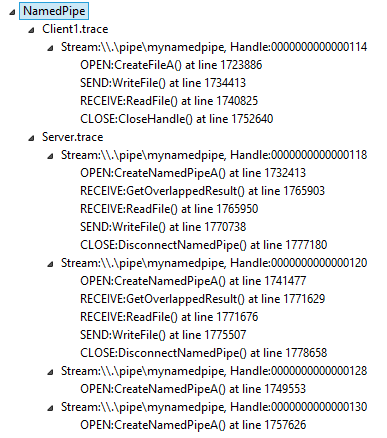
\includegraphics{Figures/result21_streams}}
 \caption{Extracted streams of $dual\_trace\_21$}
\label{result21_streams}
\end{figure}

\subsubsection{$\boldsymbol{Client1.trace:}$}
$Client1.trace$ has 1,764,281 instruction lines. Four function call events were reconstructed from this trace as listed in Table \ref{funcclient1exp2}.

\begin{table}[H]
  \centering
  \tiny
  \caption{The sequence of function call events of $Client1.trace$}
  \label{funcclient1exp2}
  \begin{tabular}{|l|p{16cm}|}
  \hline
\textbf{Line} & \multicolumn{1}{>{\centering\arraybackslash}m{16cm}|}{\textbf{Event}}\\
  \hline
  1723886 & $funN:CreateFileA,  type:open, inparams:\lbrace Handle:0x114, FileName:``\dot \backslash pipe \backslash mynamepipe" \rbrace, outparams:\lbrace RetVal:0 \rbrace$\\
 \hline
  1734413 & $funN:WriteFile, type:send, inparams:\lbrace Handle:0x114, SendBuf:``Message\:1"\rbrace, outparams: \lbrace Length:15 \rbrace$\\
\hline
 1740825&$funN:ReadFile, type:receive, inparams: \lbrace Handle:0x114 \rbrace, outparams: \lbrace RecvBuf:``Default\; answer\; from \; server", Length:17, RetVal:0 \rbrace$\\
\hline
 1752640&$funN:CloseHandle, type:close, inparams: \lbrace Handle:0x114 \rbrace, outparams: \lbrace RetVal:0 \rbrace$\\
\hline               
  \end{tabular}
\end{table}

All the values of the handle parameter of these four events are $0x114$. So a stream was extracted, which consists of all these four function call events. The extracted stream was listed in the left table  of ``Communication view"  as shown in Figure \ref{result21_streams}.

\subsubsection{$\boldsymbol{Client2.trace:}$}
$Client2.trace$ has 1764441 instruction lines. Four function call events were reconstructed from this trace as listed in Table \ref{funcclient2exp2}.

\begin{table}[H]
  \centering
  \tiny
  \caption{The sequence of function call events of $Client2.trace$}
  \label{funcclient2exp2}
  \begin{tabular}{|l|p{16cm}|}
  \hline
\textbf{Line} & \multicolumn{1}{>{\centering\arraybackslash}m{16cm}|}{\textbf{Event}}\\
  \hline
  1723886 & $funN:CreateFileA,  type:open, inparams:\lbrace Handle:0x114, FileName:``\dot \backslash pipe \backslash mynamepipe" \rbrace, outparams:\lbrace RetVal:0 \rbrace$\\
 \hline
  1734413 & $funN:WriteFile, type:send, inparams:\lbrace Handle:0x114, SendBuf:``Message\:2"\rbrace, outparams: \lbrace Length:15 \rbrace$\\
\hline
 1740825&$funN:ReadFile, type:receive, inparams: \lbrace Handle:0x114 \rbrace, outparams: \lbrace RecvBuf:``Default\; answer\; from \; server", Length:17, RetVal:0 \rbrace$\\
\hline
 1752800&$funN:CloseHandle, type:close, inparams: \lbrace Handle:0x114 \rbrace, outparams: \lbrace RetVal:0 \rbrace$\\
\hline               
  \end{tabular}
\end{table}

All the values of the handle parameter of these four events are $0x114$. So a stream was extracted, which consists of all these four function call events. 

\begin{figure}[H]
\centerline{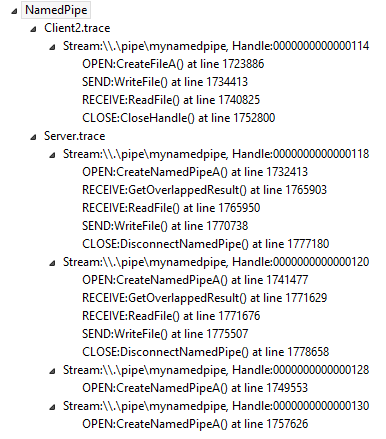
\includegraphics{Figures/result22_streams}}
 \caption{Extracted streams of $dual\_trace\_22$}
\label{result22_streams}
\end{figure}

\subsubsection{$\boldsymbol{Dual\_trace\_21:}$}
The value of the $FileName$ parameter of the $CreateFileA$ function call event in $Client1.trace$ is $``.\backslash pipe \backslash mynamepipe"$ as shown in Table \ref{funcclient1exp2}. Meanwhile, the values of the $FileName$ parameter of the $CreateNamePipeA$ function call events of all streams in $Server.trace$ are also $``.\backslash pipe \backslash mynamepipe"$ as shown in Table \ref{funcserverexp2}, so, the stream of $Client.trace$ is matched to all the streams of $Server.trace$.

The send and receive packet contents and the payload concatenation of the streams in the server and client 1 are shown in Table \ref{contentresult21}. Comparing the concatenation of each stream in $Server.trace$, it is obvious that the send payload concatenation of Stream $0x114$ in $Client1.trace$ matches the receive payload concatenation of Stream $0x120$ in $Server.trace$, while on the other direction, the send payload concatenation of Stream $0x120$ in $Server.trace$ matches the receive payload concatenation of Stream $0x114$ in $Client1.trace$, so, only Stream $0x120$ of $Server.trace$ and Stream $0x114$ of $Client1.trace$ satisfy the content preservation of the reliable communication. 

\begin{table}[H]
  \tiny
  \centering
  \caption{Content summarize of the extracted streams}
  \label{contentresult21}
  \begin{tabular}{|l|l|l|l|l|l|}
\hline            
& \multirow{2}{*}{\textbf{Handle}} & \multicolumn{2}{c|}{\textbf{Receive} }&\multicolumn{2}{c|}{\textbf{Send}} \\
\cline{3-6}
& &\multicolumn{1}{c|}{ \textbf{Events} }&\multicolumn{1}{c|}{\textbf{ Concatenation}}&\multicolumn{1}{c|}{ \textbf{Events} }&\multicolumn{1}{c|}{\textbf{ Concatenation}}\\
\hline 
\multirow{6}{*}{$\boldsymbol{Server.trace}$} &\multirow{2}{*}{$0x118$} & $GetOverlappedResult:``"$ & \multirow{2}{*}{$``Message\; 2"$} & $WriteFile:``Default\; "$ &  $``Default\; answer\; "$\\
\cline{3-3}
& &$ReadFile:``Message\; 2"$ &  & $answer\; from\; server"$&$from\; server"$\\
\cline{2-6}    
      &\multirow{2}{*}{$0x120$} & $GetOverlappedResult:``"$ & \multirow{2}{*}{$``Message\; 1"$} & $WriteFile:``Default\; $ &  $``Default\; answer\; "$\\
\cline{3-3}
& &$ReadFile:``Message\; 1"$ & &$answer\; from\; server"$ &$from\; server"$\\  
\cline{2-6}   
& $0x128$&\multicolumn{1}{c|}{- }&\multicolumn{1}{c|}{- } &\multicolumn{1}{c|}{- } &\multicolumn{1}{c|}{- }\\  
\cline{2-6}   
& $0x130$&\multicolumn{1}{c|}{- } &\multicolumn{1}{c|}{- } &\multicolumn{1}{c|}{- } &\multicolumn{1}{c|}{- }\\      
\hline  
\multirow{2}{*}{$\boldsymbol{Client1.trace}$ }&\multirow{2}{*}{$0x114$ }& $ReadFile: ``Default\; $ & $``Default\; answer\; $ & \multirow{2}{*}{$WriteFile:``Message\; 1"$ } &  \multirow{2}{*}{$``Message\; 1"$}\\
& &$answer\; from\; server"$& $ from\; server"$ & &\\
\hline
  \end{tabular}
\end{table}

Therefore, Stream $0x120$ of $Server.trace$ and Stream $0x114$ of $Client1.trace$ are eventually output as a communication by the ``Communication Identification" operation in the right table of ``Communication view" as shown in Figure \ref{result21_communications}. 

\begin{figure}[H]
\centerline{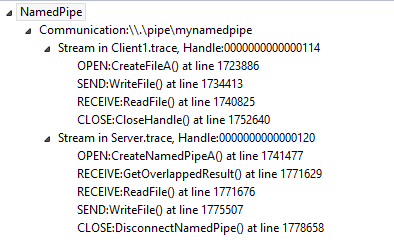
\includegraphics{Figures/result21_communications}}
 \caption{Identified communication of $dual\_trace\_21$}
\label{result21_communications}
\end{figure}

After I received the identified communication from $dual\_trace\_21$, I navigated from the send and receive events back to the traces. The navigation results are shown in Figure \ref{result21_server_readnull},  Figure \ref{result21_client_to_server} and Figure \ref{result21_server_to_client}.

\begin{figure}[H]
\DIFdelbeginFL %DIFDELCMD < \centerline{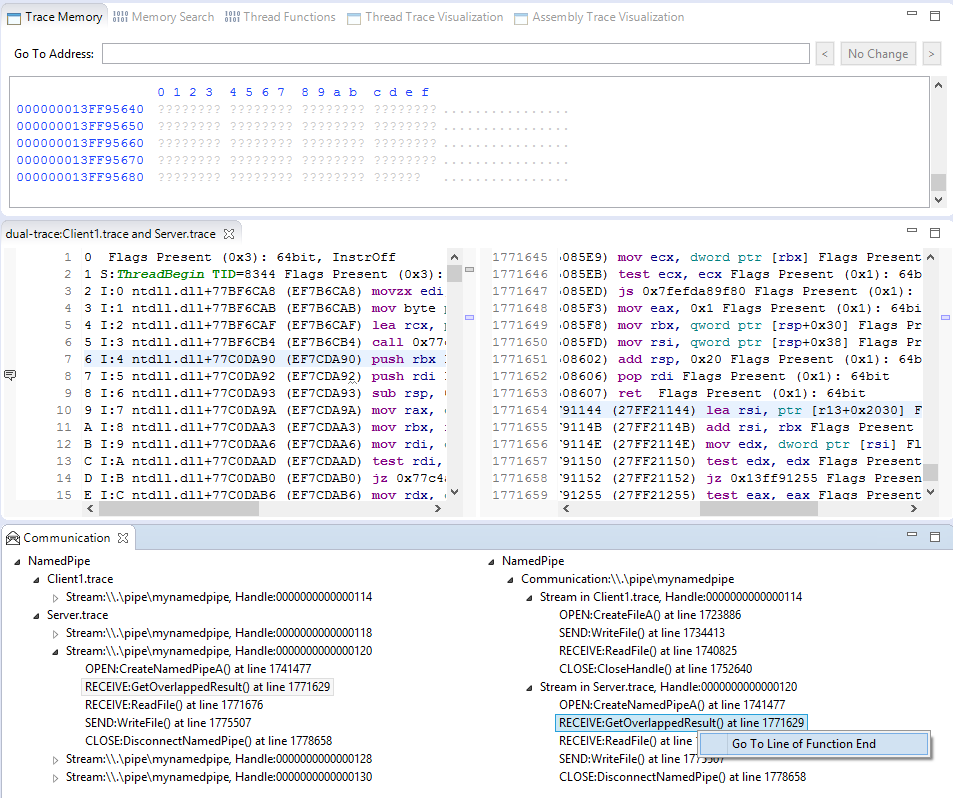
\includegraphics[scale=0.35]{Figures/result21_server_readnull}}
%DIFDELCMD <  %%%
\DIFdelendFL \DIFaddbeginFL \centerline{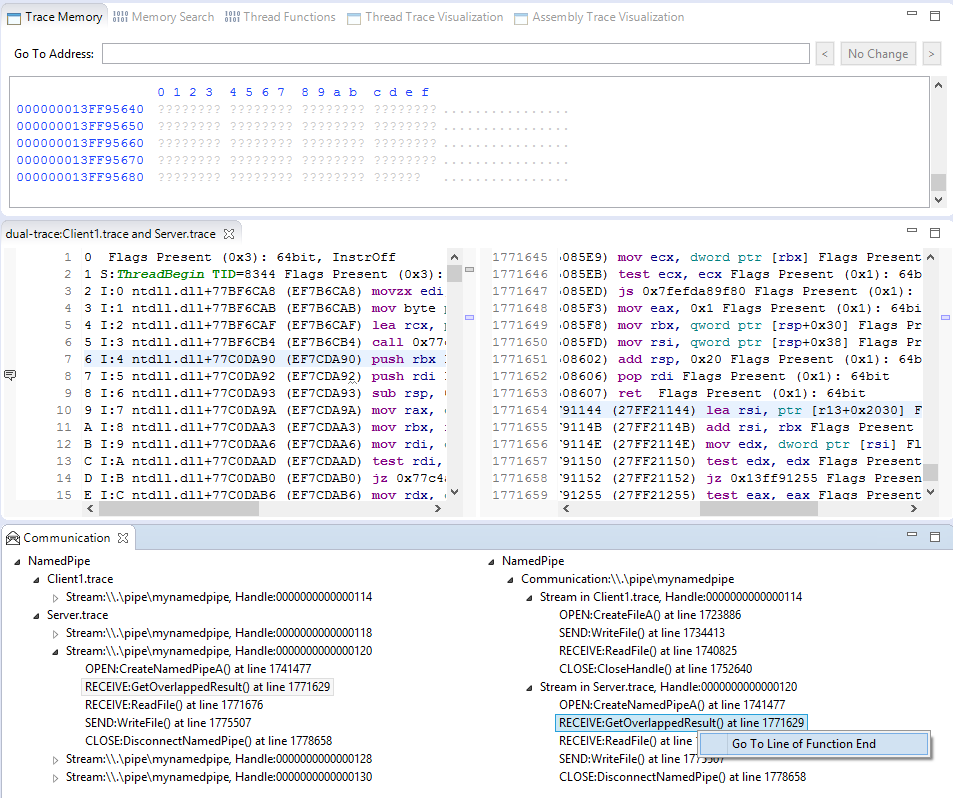
\includegraphics[scale=0.7]{Figures/result21_server_readnull}}
 \DIFaddendFL \caption{Navigation result for the function call event: $GetOverlappedResult$}
\label{result21_server_readnull}
\end{figure}

Figure \ref{result21_server_readnull} shows when I selected ``Go To Line of Function End" in the right click menu on the $GetOverlappedResult$ function call event of the $Server.trace$, it brought me to the ``Trace view" of the $Server.trace$ on line 1771653 where the function returned. However, since this function call didn't get any message, the ``Trace Memory view" is blank.


\DIFdelbegin %DIFDELCMD < \begin{figure}[H]
%DIFDELCMD < \begin{subfigure}[H]{0.45\linewidth}
%DIFDELCMD < 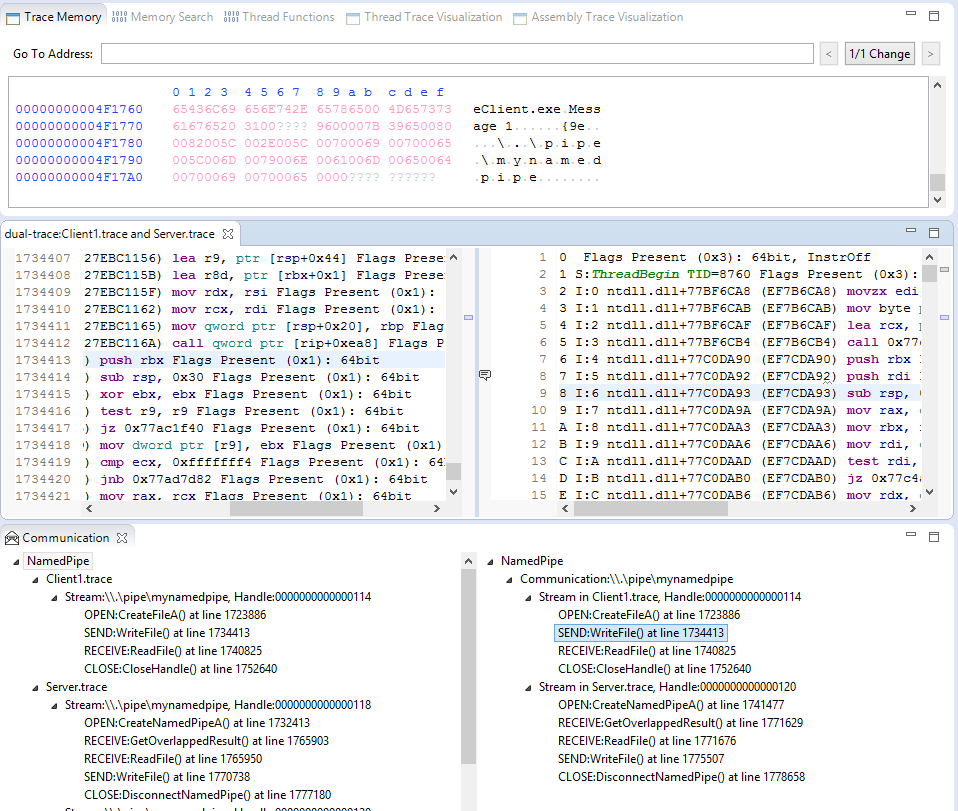
\includegraphics[scale=0.35]{Figures/result21_client_send}
%DIFDELCMD <  %%%
\DIFdelendFL \DIFaddbeginFL \begin{figure}
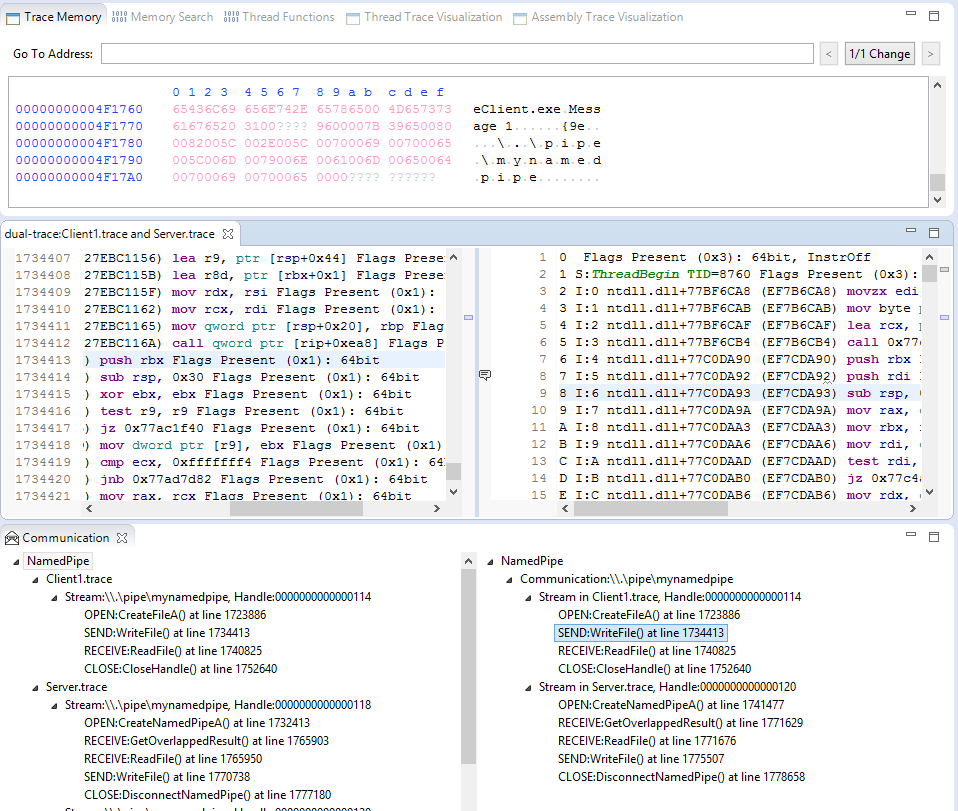
\includegraphics[scale=0.7]{Figures/result21_client_send}
 \DIFaddendFL \caption{Client 1 send event navigation \DIFaddbeginFL \DIFaddFL{for the message $``Message\; 1"$}\DIFaddendFL }
\label{result21_client_send}
\DIFdelbeginFL %DIFDELCMD < \end{subfigure}
%DIFDELCMD < \hfill
%DIFDELCMD < \begin{subfigure}[H]{0.45\linewidth}
%DIFDELCMD < 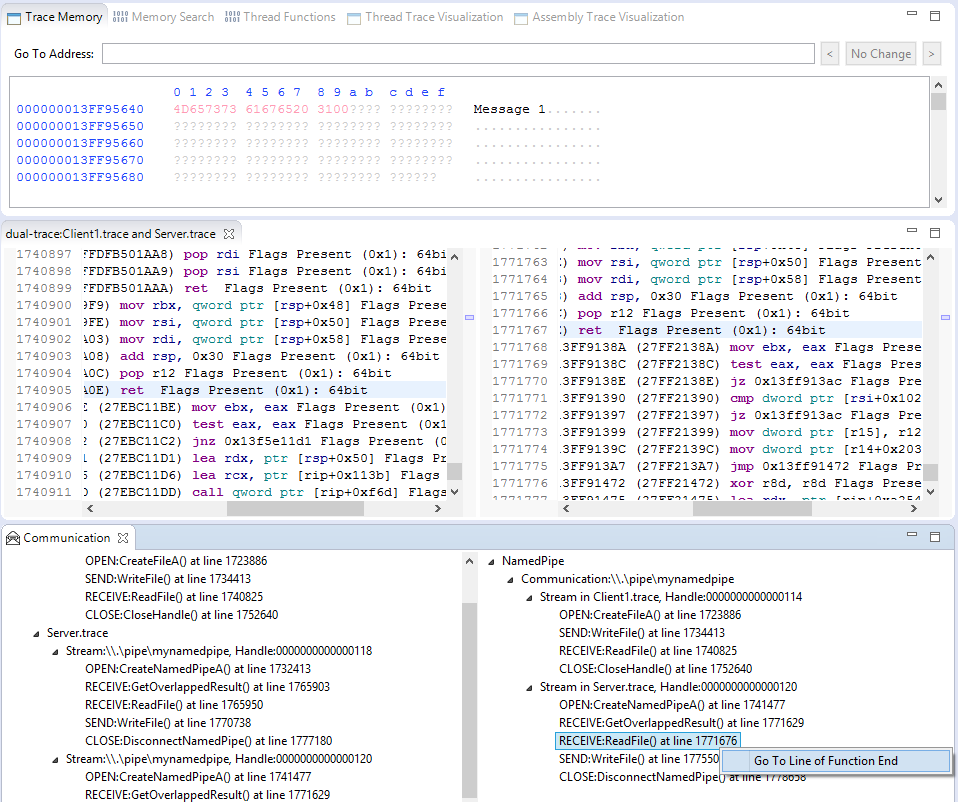
\includegraphics[scale=0.35]{Figures/result21_server_read}
%DIFDELCMD <  %%%
\DIFdelendFL \DIFaddbeginFL \end{figure}

\begin{figure}
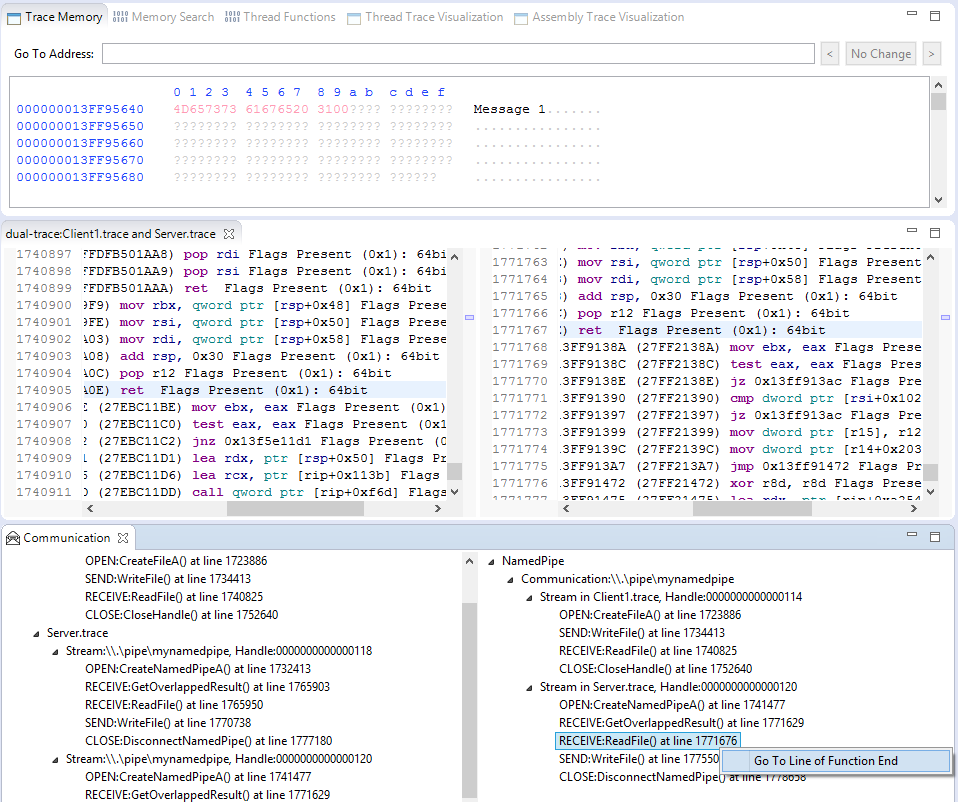
\includegraphics[scale=0.7]{Figures/result21_server_read}
 \DIFaddendFL \caption{Sever receive event navigation \DIFaddbeginFL \DIFaddFL{for the message $``Message\; 1"$}\DIFaddendFL }
\label{result21_server_read}
\DIFdelbeginFL %DIFDELCMD < \end{subfigure}%%%
%DIF < 
%DIFDELCMD < \caption{%
{%DIFAUXCMD
\DIFdelFL{Navigation results for the transmitted message $``Message\; 1"$}}
%DIFAUXCMD
%DIFDELCMD < \label{result21_client_to_server}
%DIFDELCMD < %%%
\DIFdelendFL \end{figure}

Figure \ref{result21_client_send} shows when I double clicked on the $WriteFile$ function call event of $Client.trace$, it brought me to the ``Trace view" of $Client.trace$ on line 1734413 where the function started, and the ``Trace Memory view" jumped to the memory address $0x4F176c$, which is the address for the send buffer of the message $``Message\; 1"$.

Figure \ref{result21_server_read} shows when I selected ``Go To Line of Function End" in the right click menu on the $ReadFile$ function call event of the $Server.trace$, it brought me to the ``Trace view" of the $Server.trace$ on line 1771767 where the function returned, and the ``Trace Memory view" jumped to the memory address $0x13FF95640$, which is the address for the receive buffer of the message $``Message\; 1"$.

This two figures perfectly show how the message $``Message\; 1"$ is transmitted from the client 1 to the server.

\DIFdelbegin %DIFDELCMD < \begin{figure}[H]
%DIFDELCMD < \begin{subfigure}[H]{0.45\linewidth}
%DIFDELCMD < 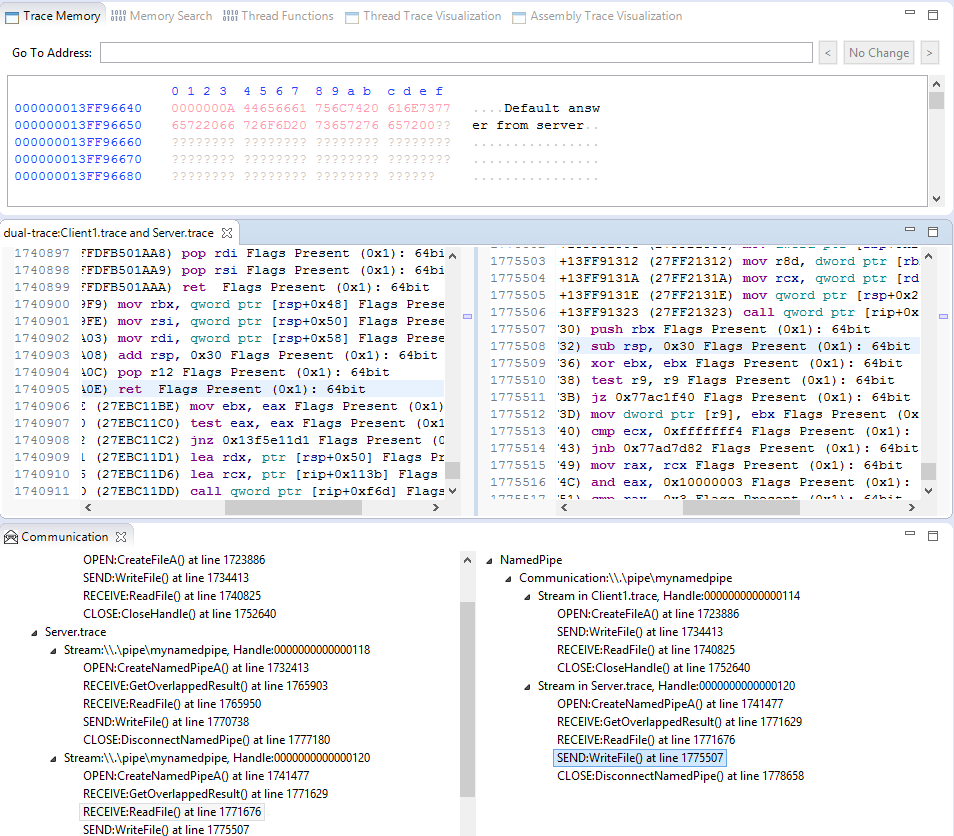
\includegraphics[scale=0.35]{Figures/result21_server_send}
%DIFDELCMD <  %%%
\DIFdelendFL \DIFaddbeginFL \begin{figure}
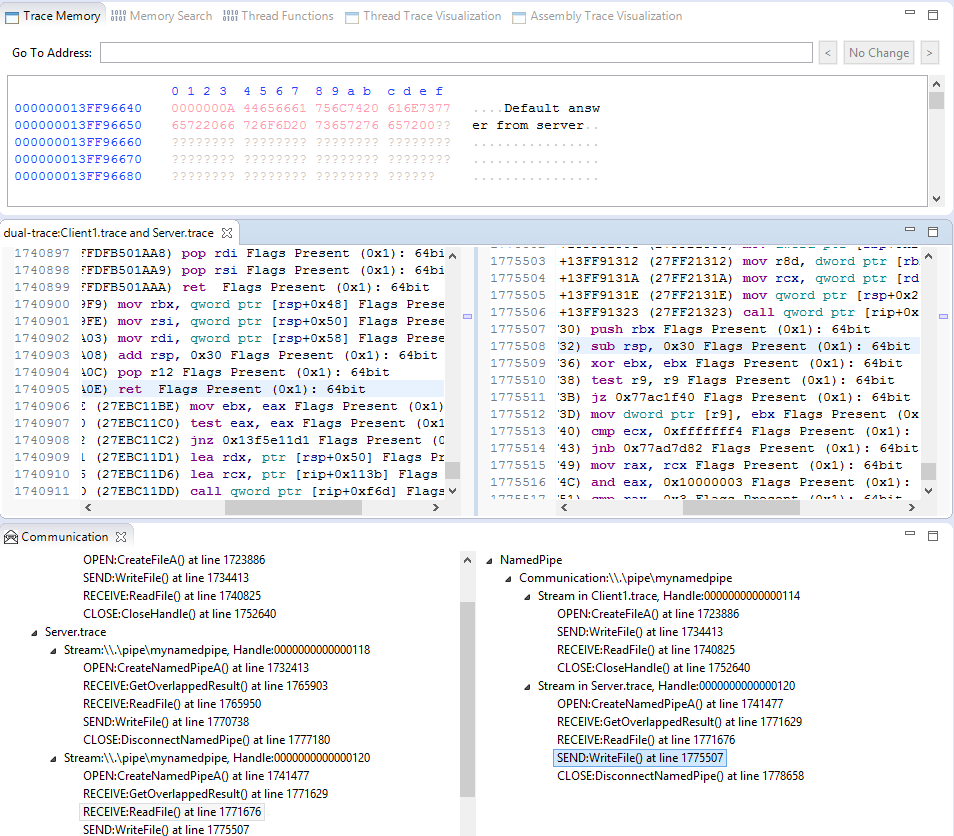
\includegraphics[scale=0.7]{Figures/result21_server_send}
 \DIFaddendFL \caption{Server send event navigation \DIFaddbeginFL \DIFaddFL{for the message $``Default\; answer\; from\; server"$}\DIFaddendFL }
\label{result21_server_send}
\DIFdelbeginFL %DIFDELCMD < \end{subfigure}
%DIFDELCMD < \hfill
%DIFDELCMD < \begin{subfigure}[H]{0.45\linewidth}
%DIFDELCMD < \includegraphics[scale=0.35]{Figures/result21_client_read}
%DIFDELCMD <  %%%
\DIFdelendFL \DIFaddbeginFL \end{figure}

\begin{figure}
\includegraphics[scale=0.7]{Figures/result21_client_read}
 \DIFaddendFL \caption{Client 1 receive event navigation \DIFaddbeginFL \DIFaddFL{for the message $``Default\; answer\; from\; server"$}\DIFaddendFL }
\label{result21_client_read}
\DIFdelbeginFL %DIFDELCMD < \end{subfigure}%%%
%DIF < 
%DIFDELCMD < \caption{%
{%DIFAUXCMD
\DIFdelFL{Navigation results for the transmitted message $``Default\; answer\; from\; server"$}}
%DIFAUXCMD
%DIFDELCMD < \label{result21_server_to_client}
%DIFDELCMD < %%%
\DIFdelendFL \end{figure}

Figure \ref{result21_server_send} shows when I double clicked on the $WriteFile$ function call event of $Server.trace$, it brought me to the ``Trace view" of $Server.trace$ on line 1775507 where the function started, and the ``Trace Memory view" jumped to the memory address $0x30EF50$, which is the address for the send buffer of the message $``Default\; answer\; from\; server"$.

Figure \ref{result21_client_read} shows when I selected ``Go To Line of Function End" in the right click menu on the $ReadFile$ function call event of $Client.trace$, it brought me to the ``Trace view" of $Client.trace$ on line 1740905 where the function returned, and the ``Trace Memory view" jumped to the memory address $0x1DF5A0$ of the receive buffer of the message $``Default\; answer\; from\; server"$.

This two figures perfectly show how the message $``Default\; answer\; from\; server"$ is transmitted from the server to the client 1.

\subsubsection{$\boldsymbol{Dual\_trace\_22:}$}
Similar to $dual\_trace\_22$, all streams of $Server.trace$ will be matched to only one stream of $Client2.trace$ by the stream matching algorithm.

The send and receive packet contents and the payload concatenation of the streams in the server and client 1 are listed in Table \ref{contentresult22}. Comparing the concatenation of each stream in $Server.trace$, it is obvious that the send payload concatenation of Stream $0x114$ in $Client2.trace$ matches the receive payload concatenation of Stream $0x118$ in $Server.trace$, while in the other direction, the send payload concatenation of Stream $0x118$ in $Server.trace$ matches the receive payload concatenation of Stream $0x114$ in $Client2.trace$ so, only Stream $0x118$ of $Server.trace$ and Stream $0x114$ of $Client2.trace$ satisfy the content preservation of the reliable communication. 

\begin{table}[H]
  \tiny
  \centering
  \caption{Content summarize of the extracted streams}
  \label{contentresult22}
  \begin{tabular}{|l|l|l|l|l|l|}
\hline            
& \multirow{2}{*}{\textbf{Handle}} & \multicolumn{2}{c|}{\textbf{Receive} }&\multicolumn{2}{c|}{\textbf{Send}} \\
\cline{3-6}
& &\multicolumn{1}{c|}{ \textbf{Events} }&\multicolumn{1}{c|}{\textbf{ Concatenation}}&\multicolumn{1}{c|}{ \textbf{Events} }&\multicolumn{1}{c|}{\textbf{ Concatenation}}\\
\hline 
\multirow{6}{*}{$\boldsymbol{Server.trace}$} &\multirow{2}{*}{$0x118$} & $GetOverlappedResult:``"$ & \multirow{2}{*}{$``Message\; 2"$} & $WriteFile:``Default\; "$ &  $``Default\; answer\; "$\\
\cline{3-3}
& &$ReadFile:``Message\; 2"$ &  & $answer\; from\; server"$&$from\; server"$\\
\cline{2-6}    
      &\multirow{2}{*}{$0x120$} & $GetOverlappedResult:``"$ & \multirow{2}{*}{$``Message\; 1"$} & $WriteFile:``Default\; $ &  $``Default\; answer\; "$\\
\cline{3-3}
& &$ReadFile:``Message\; 1"$ & &$answer\; from\; server"$ &$from\; server"$\\  
\cline{2-6}   
& $0x128$&\multicolumn{1}{c|}{- }&\multicolumn{1}{c|}{- } &\multicolumn{1}{c|}{- } &\multicolumn{1}{c|}{- }\\  
\cline{2-6}   
& $0x130$&\multicolumn{1}{c|}{- } &\multicolumn{1}{c|}{- } &\multicolumn{1}{c|}{- } &\multicolumn{1}{c|}{- }\\      
\hline  
\multirow{2}{*}{$\boldsymbol{Client2.trace}$ }&\multirow{2}{*}{$0x114$ }& $ReadFile: ``Default\; $ & $``Default\; answer\; $ & \multirow{2}{*}{$WriteFile:``Message\; 2"$ } &  \multirow{2}{*}{$``Message\; 2"$}\\
& &$answer\; from\; server"$& $ from\; server"$ & &\\
\hline
  \end{tabular}
\end{table}



Therefore, Stream $0x118$ of $Server.trace$ and Stream $0x114$ of $Client2.trace$ are eventually output as a communication by the ``Communication Identification" operation in the right table of ``Communication view" as shown in Figure \ref{result22_communications}. 

\begin{figure}[H]
\centerline{\includegraphics{Figures/result22_communications}}
 \caption{Identified communication of $dual\_trace\_22$}
\label{result22_communications}
\end{figure}

After I received the identified communication from $dual\_trace\_22$, I navigated from the send and receive events back to the traces. The navigation results are shown in Figure \ref{result22_server_readnull}, Figure \ref{result22_client_to_server} and Figure \ref{result22_server_to_client}.

\begin{figure}[H]
\DIFdelbeginFL %DIFDELCMD < \centerline{\includegraphics[scale=0.35]{Figures/result22_server_readnull}}
%DIFDELCMD <  %%%
\DIFdelendFL \DIFaddbeginFL \centerline{\includegraphics[scale=0.7]{Figures/result22_server_readnull}}
 \DIFaddendFL \caption{Navigation result for the function call event: $GetOverlappedResult$}
\label{result22_server_readnull}
\end{figure}

Figure \ref{result22_server_readnull} shows when I selected ``Go To Line of Function End" in the right click menu on the $GetOverlappedResult$ function call event of the $Server.trace$, it brought me to the ``Trace view" of the $Server.trace$ on line 1765927 where the function returned. However, since this function call didn't get any message, the ``Trace Memory view" is blank.

\DIFdelbegin %DIFDELCMD < \begin{figure}[H]
%DIFDELCMD < \begin{subfigure}[H]{0.45\linewidth}
%DIFDELCMD < \includegraphics[scale=0.35]{Figures/result22_client_send}
%DIFDELCMD <  %%%
\DIFdelendFL \DIFaddbeginFL \begin{figure}
\includegraphics[scale=0.7]{Figures/result22_client_send}
 \DIFaddendFL \caption{Client 2 send event navigation \DIFaddbeginFL \DIFaddFL{for the message $``Message\; 2"$}\DIFaddendFL }
\label{result22_client_send}
\DIFdelbeginFL %DIFDELCMD < \end{subfigure}
%DIFDELCMD < \hfill
%DIFDELCMD < \begin{subfigure}[H]{0.45\linewidth}
%DIFDELCMD < \includegraphics[scale=0.35]{Figures/result22_server_read}
%DIFDELCMD <  %%%
\DIFdelendFL \DIFaddbeginFL \end{figure}

\begin{figure}
\includegraphics[scale=0.7]{Figures/result22_server_read}
 \DIFaddendFL \caption{Sever receive event navigation \DIFaddbeginFL \DIFaddFL{for the message $``Message\; 2"$}\DIFaddendFL }
\label{result22_server_read}
\DIFdelbeginFL %DIFDELCMD < \end{subfigure}%%%
%DIF < 
%DIFDELCMD < \caption{%
{%DIFAUXCMD
\DIFdelFL{Navigation results for the transmitted message $``Message\; 2"$}}
%DIFAUXCMD
%DIFDELCMD < \label{result22_client_to_server}
%DIFDELCMD < %%%
\DIFdelendFL \end{figure}

Figure \ref{result22_client_send} shows when I double clicked on the $WriteFile$ function call event of $Client.trace$, it brought me to the ``Trace view" of $Client.trace$ on line 1734413 where the function started, and the ``Trace Memory view" jumped to the memory address $0x45176c$, which is the address for the send buffer of the message $``Message\; 2"$.

Figure \ref{result22_server_read} shows when I selected ``Go To Line of Function End" in the right click menu on the $ReadFile$ function call event of the $Server.trace$, it brought me to the ``Trace view" of the $Server.trace$ on line 1766041 where the function returned, and the ``Trace Memory view" jumped to the memory address $0x13FF93608$, which is the address for the receive buffer of the message $``Message\; 2"$.

These two figures show how the message $``Message\; 2"$ is transmitted from the client 2 to the server.



\DIFdelbegin %DIFDELCMD < \begin{figure}[H]
%DIFDELCMD < \begin{subfigure}[H]{0.45\linewidth}
%DIFDELCMD < \includegraphics[scale=0.35]{Figures/result22_server_send}
%DIFDELCMD <  %%%
\DIFdelendFL \DIFaddbeginFL \begin{figure}
\includegraphics[scale=0.7]{Figures/result22_server_send}
 \DIFaddendFL \caption{Server send event navigation \DIFaddbeginFL \DIFaddFL{for the message $``Default\; answer\; from\; server"$}\DIFaddendFL }
\label{result22_server_send}
\DIFdelbeginFL %DIFDELCMD < \end{subfigure}
%DIFDELCMD < \hfill
%DIFDELCMD < \begin{subfigure}[H]{0.45\linewidth}
%DIFDELCMD < \includegraphics[scale=0.35]{Figures/result22_client_read}
%DIFDELCMD <  %%%
\DIFdelendFL \DIFaddbeginFL \end{figure}

\begin{figure}
\includegraphics[scale=0.7]{Figures/result22_client_read}
 \DIFaddendFL \caption{Client 2 receive event navigation \DIFaddbeginFL \DIFaddFL{for the message $``Default\; answer\; from\; server"$}\DIFaddendFL }
\label{result22_client_read}
\DIFdelbeginFL %DIFDELCMD < \end{subfigure}%%%
%DIF < 
%DIFDELCMD < \caption{%
{%DIFAUXCMD
\DIFdelFL{Navigation results for the transmitted message $``Default\; answer\; from\; server"$}}
%DIFAUXCMD
%DIFDELCMD < \label{result22_server_to_client}
%DIFDELCMD < %%%
\DIFdelendFL \end{figure}

Figure \ref{result22_server_send} shows when I double clicked on the $WriteFile$ function call event of the $Server.trace$, it brought me to the ``Trace view" of the $Server.trace$ on line 1770738 where the function started, and the ``Trace Memory view" jumped to the memory address $0x13FF94608$, which is the address for the send buffer of the message $``Default\; answer\; from\; server"$.

Figure \ref{result22_client_read} shows when I selected ``Go To Line of Function End" in the right click menu on the $ReadFile$ function call event of $Client.trace$, it brought me to the ``Trace view" of $Client.trace$ on line 1740906 where the function returned, and the ``Trace Memory view" jumped to the memory address $0x2BF540$ of the receive buffer of the message $``Default\; answer\; from\; server"$.

These two figures perfectly show how the message $``Default\; answer\; from\; server"$ is transmitted from the server to the client 2.

\section{Conclusion}
By walking through the analysis results of the ``Stream Extraction" and ``Communication Identification" operations in these two experiments, I can conclude that ``Stream Extraction" operation is capable of properly extracting the streams from both traces in a dual\_trace, while ``Communication Identification" operation is capable of identifying the communication between the two traces of a dual\_trace. 

Moreover, from the ``Communication view", the user can easily navigate back to the exact instruction line where the function start or end. The messages transmitted can be shown in the ``Trace Memory view" accurately.

These two experiments are not provided as an empirical evaluation but it shows the usefulness of the algorithms and the prototype implementation.







   





	\startchapter{Conclusions and Future Work}
\label{concl}
This thesis illustrates a novel idea and an approach for dynamic program analysis which considers the interaction of two programs. This idea is valuable due to the fact that programs or malware in the real world work collaboratively. The analysis of the communication and interaction of the programs provide more reliable information for vulnerability detection and program analysis.

In this thesis, I presented an approach to analyze two traces to understand how they communicate with each other. I first defined a communication model. This abstract model depicts the outline of a communication between two running programs, which gives the ground rules for the communication analysis. Then I presented the  formalization of the dual\_trace. The formalization indicates that all traces comply to it can be used to conduct the communication analysis.

I also developed the algorithms for the communication identification. The developed algorithms not only solve the problem for specific communication methods but also provide clear and referable examples for developing other algorithms for other communication methods.

On top of the existing execution trace analysis environment, Atlantis, we implemented the communication identification features. These features provide the users a way to define the functions descriptor for communication methods through the configuration file. The user interface allows the users to conduct the communication identification and stream extraction from a dual trace and navigate back from the results to the views of the trace in Atlantis.  A proof of concept demonstrate feasibility and usability. 

\section{Discussion}
With the communication analysis prototype the user can reconstruct the communications easily. They need to understand the communication model to know what information they should retrieve from the traces to reconstruct the communications. Then they have to understand the communication method they want to investigate and follow the functions descriptor formalization to develop the functions descriptor for this communication method. With the functions descriptor, the user actually can use the old Atlantis (without the implementation of this prototype) to perform the analysis. They need to search for all the function calls to the functions in the functions descriptor, then manually go through all the function calls in the search results and follow the communication identification approach to match the streams by checking the parameter values from the reconstructed memory state of the instruction lines. This manual analysis can be extremely tedious and exhausting. In some situation, there might be a lot of communication captured in the traces and each of these communications contain a lot of message exchanges. So manually performing the analysis could be an infeasible task.

The communication identified from the dual\_trace give the necessary information, such as the transmitted data, the sequence of the packets of the communication. This provides the user a whole picture of a communication. This would be helpful for the users who need to understand how the data flow between the programs and might also help them to understand the architecture of the system. 

There are two main limitation of this work: 1) the identified communications might be errors, and 2) the user need to specify the communication method for the analysis. This means the user must be an expert who understand all the possible communications that would happen between the two programs. For example, if the user doesn't indicate that the two interacting programs communicated through TCP sockets, the communications cannot be identified. 

In conclusion, even though has limitations, this work is novel and shows its value for guiding the communication analysis through assembly-level execution traces. In addition, the prototype is the unique tool at the time of writing for the communication analysis in assembly-level.

\section{Future Works}

Future works includes:
\begin{itemize}
\item Extend the model to be more generalize for all kinds of interaction, not only the message transferring communications, for example remote procedure call
\item Visualize the communications identified from the dual\_trace (a sequence diagram might be a good choice to illustrate all the events in the traces and the matched events from both traces.) 
\item Conduct user studies of the communication analysis approach and the prototype (user observation for tasks performing with the prototype and follow-up interview)
\item Conduct an empirical study to properly evaluate the algorithms and implementation presented in this thesis (run some applications that contain known vulnerabilities that are related to communication and see if the communication identification can assist the analyst to detect these vulnerabilities.)
\end{itemize}

Accomplish of the first two future works can make the communication analysis method developed in this work more complete. The last two future works can validate the usefulness and Usability of this work.




	\TOCadd{Bibliography}
	\bibliographystyle{plain}
	\begin{thebibliography}{10}

\bibitem{bhansali2006framework}
Sanjay Bhansali, Wen-Ke Chen, Stuart De~Jong, Andrew Edwards, Ron Murray,
  Milenko Drini{\'c}, Darek Miho{\v{c}}ka, and Joe Chau.
\newblock Framework for instruction-level tracing and analysis of program
  executions.
\newblock In {\em Proceedings of the 2nd international conference on Virtual
  execution environments}, pages 154--163. ACM, 2006.

\bibitem{brueningqz}
Derek Bruening.
\newblock Qz: Dynamorio: Dynamic instrumentation tool platform.
\newblock \url{http://www.dynamorio.org/}.

\bibitem{cai2016sworddta}
Jun Cai, Peng Zou, Jinxin Ma, and Jun He.
\newblock Sworddta: A dynamic taint analysis tool for software vulnerability
  detection.
\newblock {\em Wuhan University Journal of Natural Sciences}, 21(1):10--20,
  2016.

\bibitem{_wireshark_????}
Gerald Combs.
\newblock Wireshark · {Go} {Deep}.
\newblock \url{https://www.wireshark.org/}.

\bibitem{_c0demap/codemap:_????}
KAIST CysecLab.
\newblock Codemap.
\newblock \url{https://github.com/c0demap/codemap}.

\bibitem{dowd_art_2006}
Mark Dowd, John McDonald, and Justin Schuh.
\newblock {\em Art of {Software} {Security} {Assessment}, {The}: {Identifying}
  and {Preventing} {Software} {Vulnerabilities}}.
\newblock Addison-Wesley Professional., 1st edition, November 2006.

\bibitem{eagle_ida_2008}
Chris Eagle.
\newblock {\em The {IDA} {Pro} {Book}: {The} {Unofficial} {Guide} to the
  {World}'s {Most} {Popular} {Disassembler}}.
\newblock No Starch Press, San Francisco, CA, USA, 2008.

\bibitem{garrido2000inter}
Jos{\'e}~M Garrido.
\newblock Inter-process communication.
\newblock {\em Performance Modeling of Operating Systems Using Object-Oriented
  Simulation: A Practical Introduction}, pages 169--189, 2000.

\bibitem{gcc}
GCC.
\newblock Options that control optimization.
\newblock
  \url{https://gcc.gnu.org/onlinedocs/gcc-4.9.1/gcc/Optimize-Options.html}.

\DIFaddbegin \bibitem{hansman2005taxonomy}

Michael Howard and David LeBlanc.
\newblock {\em Writing secure code}.
\newblock Pearson Education, 2003.

\bibitem{huang2017atlantis}
Huihui~Nora Huang, Eric Verbeek, Daniel German, Margaret-Anne Storey, and
  Martin Salois.
\newblock Atlantis: Improving the analysis and visualization of large assembly
  execution traces.
\newblock In {\em Software Maintenance and Evolution (ICSME), 2017 IEEE
  International Conference on}, pages 623--627. IEEE, 2017.

\bibitem{_pin_????}
Intel.
\newblock Pin - {A} {Dynamic} {Binary} {Instrumentation} {Tool}.
\newblock
  \url{https://software.intel.com/en-us/articles/pin-a-dynamic-binary-instrumentation-tool}.

\DIFaddbegin 

\bibitem{leavitt2011mobile}


\bibitem{WinMSMQ}
MSDN.
\newblock Message queue (windows).
\newblock
  \url{https://msdn.microsoft.com/en-us/library/ms705205(v=vs.85).aspx}.

\bibitem{WinNamedpipe}
MSDN.
\newblock Named pipes (windows).
\newblock
  \url{https://msdn.microsoft.com/en-us/library/windows/desktop/aa365590(v=vs.85).aspx}.

\bibitem{winsock}
MSDN.
\newblock Socket reference (windows).
\newblock
  \url{https://msdn.microsoft.com/en-us/library/windows/desktop/ms741416(v=vs.85).aspx}.

\bibitem{redkar2004pro}
Arohi Redkar, Ken Rabold, Richard Costall, Scot Boyd, and Carlos Walzer.
\newblock {\em Pro MSMQ: Microsoft Message Queue Programming}.
\newblock Apress, 2004.

\bibitem{somorovsky2016systematic}
Juraj Somorovsky.
\newblock Systematic fuzzing and testing of tls libraries.
\newblock In {\em Proceedings of the 2016 ACM SIGSAC Conference on Computer and
  Communications Security}, pages 1492--1504. ACM, 2016.

\bibitem{tcpdump_tcpdump/libpcap_????}
Tcpdump.
\newblock Tcpdump/{Libpcap} public repository.
\newblock \url{http://www.tcpdump.org}.

\bibitem{trumper2012maintenance}
Jonas Tr{\"u}mper, Stefan Voigt, and J{\"u}rgen D{\"o}llner.
\newblock Maintenance of embedded systems: Supporting program comprehension
  using dynamic analysis.
\newblock In {\em Software Engineering for Embedded Systems (SEES), 2012 2nd
  International Workshop on}, pages 58--64. IEEE, 2012.

\bibitem{wen2017model}
Shameng Wen, Qingkun Meng, Chao Feng, and Chaojing Tang.
\newblock A model-guided symbolic execution approach for network protocol
  implementations and vulnerability detection.
\newblock {\em PloS one}, 12(11):e0188229, 2017.

\bibitem{yuschuk2007ollydbg}
Oleh Yuschuk.
\newblock Ollydbg.
\newblock \url{http://www.ollydbg.de/}, 2007.

\bibitem{zhang2010detecting}
Dazhi Zhang, Donggang Liu, Yu~Lei, David Kung, Christoph Csallner, and Wenhua
  Wang.
\newblock Detecting vulnerabilities in c programs using trace-based testing.
\newblock In {\em Dependable Systems and Networks (DSN), 2010 IEEE/IFIP
  International Conference on}, pages 241--250. IEEE, 2010.

\end{thebibliography}


	\begin{appendices}	
\chapter{Microsoft x64 Calling Convention for C/C++}\label{convention}
\begin{itemize}  
\item RCX, RDX, R8, R9 are used for integer and pointer arguments in that order left to right.
\item XMM0, 1, 2, and 3 are used for floating point arguments.
\item Additional arguments are pushed on the stack left to right. \ldots 
\item Parameters less than 64 bits long are not zero extended; the high bits contain garbage.
\item Integer return values (similar to x86) are returned in RAX if 64 bits or less.
\item Floating point return values are returned in XMM0.
\item Larger return values (structs) have space allocated on the stack by the caller, and RCX then contains a pointer to the return space when the callee is called. Register usage for integer parameters is then pushed one to the right. RAX returns this address to the caller.
\end{itemize}

\chapter{Function Descriptor Configuration file Example}\label{funcset}
\lstinputlisting[caption= communicationMethods.json]{./sourcecode/communicationMethods.json}

\chapter{Code of the Parallel Editors}\label{paralleleditor}
Two essential pieces of code are listed for the parallel editor. One is for splitting the editor area for two editors while the other is to get the active parallel editors later on  for dual\_trace analysis.
\section{The Editor Area Split Handler}
\begin{lstlisting}[caption= code in OpenDualEditorsHandler.java]
public class OpenDualEditorsHandler extends AbstractHandler {
	EModelService ms;
	EPartService ps;
	WorkbenchPage page;

	  
    public Object execute(ExecutionEvent event) throws ExecutionException {
		IEditorPart editorPart = HandlerUtil.getActiveEditor(event);
		if (editorPart == null) {
			Throwable throwable = new Throwable("No active editor");
			BigFileApplication.showErrorDialog("No active editor", "Please open one file first", throwable);
			return null;
		}

		MPart container = (MPart) editorPart.getSite().getService(MPart.class);
		MElementContainer m = container.getParent();
		if (m instanceof PartSashContainerImpl) {
			Throwable throwable = new Throwable("The active file is already opened in one of the parallel editors");
			BigFileApplication.showErrorDialog("TThe active file is already opened in one of the parallel editors",
					"The active file is already opened in one of the parallel editors", throwable);
			return null;
		}
		IFile file = getPathOfSelectedFile(event);

		IEditorDescriptor desc = PlatformUI.getWorkbench().getEditorRegistry().getDefaultEditor(file.getName());
		try {
			IFileUtils fileUtil = RegistryUtils.getFileUtils();
			File f = BfvFileUtils.convertFileIFile(file);
			f = fileUtil.convertFileToBlankFile(f);
			IFile convertedFile = ResourcesPlugin.getWorkspace().getRoot().getFileForLocation(Path.fromOSString(f.getAbsolutePath()));
			convertedFile.getProject().refreshLocal(IResource.DEPTH_INFINITE, null);
			if (!convertedFile.exists()) {
				createEmptyFile(convertedFile);
			}

			IEditorPart containerEditor = HandlerUtil.getActiveEditorChecked(event);
			IWorkbenchWindow window = HandlerUtil.getActiveWorkbenchWindowChecked(event);
			ms = window.getService(EModelService.class);
			ps = window.getService(EPartService.class);
			page = (WorkbenchPage) window.getActivePage();
			IEditorPart editorToInsert = page.openEditor(new FileEditorInput(convertedFile), desc.getId());
			splitEditor(0.5f, 3, editorToInsert, containerEditor, new FileEditorInput(convertedFile));
			window.getShell().layout(true, true);


		} catch (CoreException e) {
			e.printStackTrace();
		}

		return null;
	}

    private void createEmptyFile(IFile file) {
		byte[] emptyBytes = "".getBytes();
		InputStream source = new ByteArrayInputStream(emptyBytes);
		try {
			createParentFolders(file);
			if(!file.exists()){
				file.create(source, false, null);
			}
		} catch (CoreException e) {
			e.printStackTrace();
		}finally{
			try {
				source.close();
			} catch (IOException e) {
				// Don't care
			}
		}
	}

	private void splitEditor(float ratio, int where, IEditorPart editorToInsert, IEditorPart containerEditor,
			FileEditorInput newEditorInput) {
		MPart container = (MPart) containerEditor.getSite().getService(MPart.class);
		if (container == null) {
			return;
		}

		MPart toInsert = (MPart) editorToInsert.getSite().getService(MPart.class);
		if (toInsert == null) {
			return;
		}

		MPartStack stackContainer = getStackFor(container);
		MElementContainer<MUIElement> parent = container.getParent();
		int index = parent.getChildren().indexOf(container);
		MStackElement stackSelElement = stackContainer.getChildren().get(index);

		MPartSashContainer psc = ms.createModelElement(MPartSashContainer.class);
		psc.setHorizontal(true);
		psc.getChildren().add((MPartSashContainerElement) stackSelElement);
		psc.getChildren().add(toInsert);
		psc.setSelectedElement((MPartSashContainerElement) stackSelElement);

		MCompositePart compPart = ms.createModelElement(MCompositePart.class);
		compPart.getTags().add(EPartService.REMOVE_ON_HIDE_TAG);
		compPart.setCloseable(true);
		compPart.getChildren().add(psc);
		compPart.setSelectedElement(psc);
		compPart.setLabel("dual-trace:" + containerEditor.getTitle() + " and " + editorToInsert.getTitle());

		parent.getChildren().add(index, compPart);
		ps.activate(compPart);

	}

	private MPartStack getStackFor(MPart part) {
		MUIElement presentationElement = part.getCurSharedRef() == null ? part : part.getCurSharedRef();
		MUIElement parent = presentationElement.getParent();
		while (parent != null && !(parent instanceof MPartStack))
			parent = parent.getParent();

		return (MPartStack) parent;
	}


	private IFile getPathOfSelectedFile(ExecutionEvent event) {
		IWorkbenchWindow window = PlatformUI.getWorkbench().getActiveWorkbenchWindow();
		if (window != null) {
			window = HandlerUtil.getActiveWorkbenchWindow(event);
			IStructuredSelection selection = (IStructuredSelection) window.getSelectionService().getSelection();
			Object firstElement = selection.getFirstElement();
			if (firstElement instanceof IFile) {
				return (IFile) firstElement;
			}
			if (firstElement instanceof IFolder) {
				IFolder folder = (IFolder) firstElement;
				AtlantisBinaryFormat binaryFormat = new AtlantisBinaryFormat(
						folder.getRawLocation().makeAbsolute().toFile());
				// arbitrary, just any file in the binary set is needed
				return AtlantisFileUtils.convertFileIFile(binaryFormat.getExecVtableFile());
			}
		}
		return null;
	}
}
\end{lstlisting}

\section{Get the Active Parallel Editors}
\begin{lstlisting}[caption= code for getting parallel editors ]
IEditorPart editorPart = PlatformUI.getWorkbench().getActiveWorkbenchWindow().getActivePage().getActiveEditor();
		MPart container = (MPart) editorPart.getSite().getService(MPart.class);
		MElementContainer m = container.getParent();
		if (!(m instanceof PartSashContainerImpl)) {
			Throwable throwable = new Throwable("This is not a dual-trace");
			BigFileApplication.showErrorDialog("This is not a dual-trace!", "Open a dual-trace First", throwable);
			return;
		}

		MPart editorPart1 = (MPart) m.getChildren().get(0);
		MPart editorPart2 = (MPart) m.getChildren().get(1);
\end{lstlisting}

\chapter{Code of the Programs in the Experiments}\label{expcode}
\section{Experiment 1}
The two interacting programs were Named pipe server and client. The first piece of code listed below is the code for the server's program while the second piece is for the client program.
\lstinputlisting[language=C++,caption= NamedPipeServer.cpp]{./sourcecode/experiment1/NamedPipeServer.cpp}
\lstinputlisting[language=C++,caption= NamedPipeClient.cpp]{./sourcecode/experiment1/NamedPipeClient.cpp}

\section{Experiment 2}
In the experiment 2, two clients run the same program in sequence to connect to the server with asynchronous Named pipe channel. The first piece of code listed below is the code for the server's program while the second piece is the test.bat is the script for running the experiment. The client  program's code is identical to experiment 1.
\lstinputlisting[language=C++,caption= NamedPipeServerOverlapped.cpp]{./sourcecode/experiment2/NamedPipeServerOverlapped.cpp}
\lstinputlisting[caption= test.bat]{./sourcecode/experiment2/test.bat}

\end{appendices}


% The style of bibliography exemplified here is the "plain",
% normally used in science theses. This is shown
% by the entry {plain} below. Substitute the
% appropriate bibliography style. See also the
% PDF file "InformationOnBibliographyStyles" in this
% directory for more choices.

% The Bibliography file is a BibTex file named
% UVicThesis.bib and called below



\end{document}
vardef  enddefvardef  enddef